% ==============================================================================
% OVERGROWN PROJECT - MAIN OTIMIZADO (VERSÃO CORRIGIDA)
% ==============================================================================
% !TeX program = xelatex
\documentclass[10pt, a4paper, oneside]{book} 

% --- O SEGREDO DO TEMPO DE COMPILAÇÃO ---
% Descomente a linha abaixo e coloque o nome do arquivo para compilar só ele.
% \includeonly{Contents/magia/fogo}

% Importa as configurações
% config.tex
\usepackage[portuguese]{babel}
\usepackage[margin=1.5cm, bottom=2cm]{geometry}
\usepackage{multicol}
% \usepackage{lipsum}   % removido: lorem ipsum não vai para produção
\usepackage{graphicx}
\usepackage{fontspec}
\usepackage{fancyhdr}
\usepackage{lettrine}
\usepackage{titlesec}
\usepackage{comment}
\usepackage{tabularx}
\usepackage{xltabular}
\usepackage{needspace}
\usepackage{booktabs}
\usepackage[table]{xcolor}
\usepackage{tikz}
% --- OTIMIZAÇÃO: apenas a lib 'skins' (para o enhanced de \attrField).
% [most] carregava ~10 bibliotecas extras desnecessárias.

 \usepackage{amsmath}
\usepackage{tcolorbox}
\tcbuselibrary{skins}
\usepackage{etoolbox}         % para \ifstrempty em \spellCard
\usepackage{eso-pic}
\usepackage[hidelinks]{hyperref} 

% --- OTIMIZAÇÃO DE IMAGEM REPETITIVA ---
% Carrega o dado uma vez na memória em vez de ler o disco toda vez
\AddToShipoutPictureBG{%
    \AtPageLowerLeft{%
        
\includegraphics[width=\paperwidth,height=\paperheight]{Images/background.jpg}%
    }%
}

\begin{comment}
\newsavebox{\diceicon}
\savebox{\diceicon}{
\includegraphics[height=1.2em]{Images/dado.png}}

\newcommand{\dado}[2]{%
    \textbf{#1}\,%
    \begin{tikzpicture}[baseline=(ICONE.base)]
        \node[inner sep=0pt] (ICONE) {\usebox{\diceicon}};
        \node[text=white, font=\color{white}\footnotesize\bfseries] at (ICONE.center) {#2};
    \end{tikzpicture}
}

% --- BACKGROUND OTIMIZADO ---
% Se o PDF final ficar lento para rolar as páginas, o culpado é esse background.
% DICA: Converta background.png para um PDF de baixa resolução (72dpi)
\backgroundsetup{
    scale=1, color=black, opacity=1, angle=0,
    contents={
\includegraphics[width=\paperwidth,height=\paperheight]{Images/background}}
}
\end{comment}

% --- FONTES ---
\defaultfontfeatures{Ligatures=TeX}

% 1. Define the font families (the switches)
\newfontfamily\baskerfamily[
    Path=Fonts/,
    Extension=.ttf,
    BoldFont=BASKER,
    ItalicFont=BASKER,
    BoldItalicFont=BASKER
]{BASKER}
\newfontfamily\ringmfamily[
    Path=Fonts/,
    Extension=.ttf,
    BoldFont=RINGM,
    ItalicFont=RINGM,
    BoldItalicFont=RINGM
]{RINGM}

% 2. Define the text commands (the \command{text} versions)
\DeclareTextFontCommand{\basker}{\baskerfamily}
\DeclareTextFontCommand{\ringm}{\ringmfamily}

% 3. Set the main document font
\setmainfont[
    Path=Fonts/,
    Extension=.ttf,
    BoldFont=BASKER,
    ItalicFont=BASKER,
    BoldItalicFont=BASKER
]{BASKER}

\hbadness=10000
\vbadness=10000
\emergencystretch=2em

% --- Estilos de Página ---
\fancypagestyle{fancy}{
    \fancyhf{}
    \fancyfoot[R]{\ringmfamily\Large\thepage}
    \renewcommand{\headrulewidth}{0pt}
    \renewcommand{\footrulewidth}{0pt}
}

\fancypagestyle{plain}{
    \fancyhf{}
    \fancyfoot[R]{\ringmfamily\Large\thepage}
}
\pagestyle{fancy}

% --- Cores e Réguas RPG ---
\definecolor{armorGold}{HTML}{fdf1d3}
\definecolor{overgrownRed}{HTML}{8b0000}

\newcommand{\weaponRule}{%
    \begin{tikzpicture}[node distance=0pt]
        \fill[overgrownRed] (0,0) -- (0.2,0.05) -- (\linewidth-0.2cm,0.05) -- (\linewidth,0) -- (\linewidth-0.2cm,-0.05) -- (0.2,-0.05) -- cycle;
    \end{tikzpicture}%
}

\newcommand{\overRule}{%
    \par\noindent\centering
    \begin{tikzpicture}
        \fill[overgrownRed] (0,0) -- (0.1,0.03) -- (\linewidth-0.1cm,0.03) -- (\linewidth,0) -- (\linewidth-0.1cm,-0.03) -- (0.1,-0.03) -- cycle;
    \end{tikzpicture}
    \par
}

\newcommand{\blackoverRule}{%
    \par\noindent\centering
    \begin{tikzpicture}
        \fill[black] (0,0) -- (0.1,0.03) -- (\linewidth-0.1cm,0.03) -- (\linewidth,0) -- (\linewidth-0.1cm,-0.03) -- (0.1,-0.03) -- cycle;
    \end{tikzpicture}
    \par
}

% --- Widgets RPG ---
\newtcolorbox{rpgboxtips}[1]{colback=gray!10, colframe=black!70, fonttitle=\bfseries, title=#1, arc=0mm}

\newcommand{\attrField}[2]{%
    \begin{tcolorbox}[enhanced, colback=black, coltext=white, sharp corners, boxrule=0pt, width=0.485\linewidth, nobeforeafter, left=4pt, right=4pt, top=3pt, bottom=3pt, fontupper=\sffamily\bfseries\footnotesize]
    #1 \hfill \normalfont\footnotesize #2
    \end{tcolorbox}\hfill
}

\newcommand{\statBox}[2]{%
    \begin{tcolorbox}[colback=black, coltext=white, sharp corners, boxrule=0pt, width=0.18\linewidth, nobeforeafter, left=0pt, right=0pt, top=4pt, bottom=4pt, halign=center, fontupper=\sffamily\bfseries\scriptsize]
    #1 \\ \vspace{1pt} \large #2
    \end{tcolorbox}\hfill
}

% --- Espaçamentos e Títulos ---
\setlength{\parskip}{0.2cm}
\setlength{\parindent}{0pt}
\setlength{\columnsep}{1cm}
\newcommand{\column}{\columnbreak}

\titlespacing*{\section}{0pt}{10pt}{4pt}
\titlespacing*{\subsection}{0pt}{8pt}{4pt}
\titleformat{\section}{\ringmfamily\fontsize{14}{22}\selectfont}{\thesection}{1em}{}
\titleformat{\subsection}{\ringmfamily\fontsize{13}{18}\selectfont}{\thesubsection}{1em}{}

\newcommand{\midsectiontitle}[1]{%
    \needspace{5\baselineskip}%
    \begin{flushleft}%
        {\ringmfamily\fontsize{24}{32}\selectfont #1}\par
        \blackoverRule
    \end{flushleft}%
    \phantomsection
    \addcontentsline{toc}{section}{#1}%
}

% --- Sistema de Armas ---
\makeatletter
\define@key{arma}{nome}{\def\arma@nome{#1}}
\define@key{arma}{desc}{\def\arma@desc{#1}}
\define@key{arma}{ameaca}{\def\arma@ameaca{#1}}
\define@key{arma}{tipo}{\def\arma@tipo{#1}}
\define@key{arma}{peso}{\def\arma@peso{#1}}

\newcommand{\exibirPeso}[1]{#1\ Unidade\ifnum#1>1 s\fi\ de Peso}

\newcommand{\armaCard}[1]{%
    \setkeys{arma}{nome={Nome},desc={},ameaca={20},tipo={Item},peso={1},#1}%
    \vspace{3pt}\noindent
    \begin{minipage}{\linewidth}
        {\ringmfamily\Large\color{overgrownRed}\arma@nome} \hfill {\small\color{overgrownRed}AMEAÇA \arma@ameaca}\par
        \vspace{1pt}
        {\scriptsize\scshape \arma@tipo \hfill \exibirPeso{\arma@peso}}\par
        \vspace{-2pt}
        \overRule 
        \vspace{2pt}
        \ifx\arma@desc\@empty\else
            \noindent\textit{\footnotesize \arma@desc}\par
            \vspace{8pt}
        \fi
        {\ringmfamily\footnotesize\color{overgrownRed} ATAQUES E MANOBRAS}
        \vspace{2pt}
        \hrule height 0.6pt 
        \vspace{4pt}
}

\newcommand{\addAtaque}[3]{%
    \noindent\textbf{\small #1} \hfill \textbf{\small #3}\\%
    \textit{\scriptsize #2}\par\vspace{4pt}%
}

\newcommand{\finishArma}{%
    \vspace{2pt}
    \hrule height 0.4pt
    \end{minipage}
    \vspace{15pt}
}
\makeatother

% --- Hyperlinks ---

\hypersetup{colorlinks=true, linkcolor=blue, urlcolor=cyan}
\newcommand{\originlink}[1]{\phantomsection{\hypertarget{#1}{}}}
\newcommand{\link}[2]{\hyperlink{#1}{#2}}

% --- Comando de Perícias ---
\newcommand{\pericia}[2]{%
    \needspace{3\baselineskip}
    \vspace{6pt}
    \noindent
    {\ringmfamily\color{overgrownRed} #1:}\hspace{5pt}#2\par
    \vspace{4pt}
}

% --- Comando de Habilidades de Combate ---
% #1 = Nome, #2 = Custo (ex: "2" ou "X"), #3 = Descrição
\newcommand{\combatSkill}[3]{%
    \needspace{4\baselineskip}%
    \vspace{5pt}%
    \noindent%
    {\ringmfamily\color{overgrownRed}\large #1}\hfill%
    {\setlength{\fboxsep}{2pt}\small\scshape\fbox{#2\ PC}}\par%
    \vspace{2pt}%
    \noindent{\small #3}\par%
    \vspace{4pt}%
}

% --- Sistema de Armaduras (Ajustado para Armour/Bloqueio) ---
\makeatletter
\define@key{armor}{nome}{\def\armor@nome{#1}}
\define@key{armor}{tipo}{\def\armor@tipo{#1}}
\define@key{armor}{peso}{\def\armor@peso{#1}}
\define@key{armor}{vida}{\def\armor@vida{#1}}
\define@key{armor}{armour}{\def\armor@armour{#1}} % Atributo para Bloqueio

\newcommand{\armorCard}[1]{%
    \setkeys{armor}{nome={Armadura},tipo={Traje},peso={1},vida={10},armour={0},#1}%
    \vspace{12pt}\noindent
    \begin{minipage}{\linewidth}
        {\ringmfamily\Large\color{overgrownRed}\armor@nome} \hfill {\small\color{overgrownRed}ARMOUR \armor@armour}\par
        \vspace{1pt}
        {\scriptsize\scshape \armor@tipo \hfill \exibirPeso{\armor@peso}}\par
        \vspace{-2pt}
        \overRule 
        \vspace{2pt}
        \noindent\textbf{\small Vida de Armadura:} \armor@vida\ PV\par
        \vspace{4pt}
        {\ringmfamily\footnotesize\color{overgrownRed} PROPRIEDADES E EFEITOS}
        \vspace{2pt}
        \hrule height 0.6pt 
        \vspace{4pt}
}

\newcommand{\addEfeito}[2]{%
    \noindent\textbf{\small #1:} {\scriptsize #2}\par\vspace{4pt}%
}

\newcommand{\finishArmor}{%
    \vspace{2pt}
    \hrule height 0.4pt
    \end{minipage}
    \vspace{15pt}
}
\makeatother


% balões de elementos
\definecolor{elemFogo}{HTML}{E63946}
\definecolor{elemAgua}{HTML}{457B9D}
\definecolor{elemAr}{HTML}{A8DADC}
\definecolor{elemTerra}{HTML}{767522}
\definecolor{elemNatureza}{HTML}{2B9348}
\definecolor{elemLuz}{HTML}{FFB703}
\definecolor{elemSombra}{HTML}{3D348B}
\definecolor{elemEletricidade}{HTML}{8338EC}
\definecolor{elemTempo}{HTML}{FB5607}
\definecolor{elemMental}{HTML}{FF006E}
\definecolor{elemEspacial}{HTML}{023047}
\definecolor{elemInvocacao}{HTML}{8D99AE}

 
% --- OTIMIZAÇÃO CRÍTICA: \elementTag e \typeTag
% Antes: cada tag criava um tcolorbox completo (~200+ instâncias só nas spell cards).
% Agora: usa \fcolorbox nativo — mesma aparência, custo praticamente zero.

% Tag de Elemento (ex: Fogo, Agua)
\newcommand{\elementTag}[1]{%
    {\setlength{\fboxsep}{1.5pt}\setlength{\fboxrule}{0.6pt}%
    \leavevmode\hbox{\fontsize{7pt}{7pt}\selectfont\bfseries\sffamily%
    \fcolorbox{elem#1}{elem#1!15}{\color{elem#1!80!black}\MakeUppercase{#1}}}}%
    \hspace{2pt}%
}

% Tag de Tipo (ex: PROJ, AOE, BUFF)
\newcommand{\typeTag}[1]{%
    {\setlength{\fboxsep}{1.2pt}\setlength{\fboxrule}{0.6pt}%
    \leavevmode\hbox{\fontsize{6pt}{6pt}\selectfont\bfseries\sffamily%
    \fcolorbox{black!60}{white}{\color{black!90}#1}}}%
    \hspace{2pt}%
}

% Card de Magia Atualizado
% Parâmetros: 
% #1 Nome, #2 Elementos, #3 DIV+, #4 Descrição, #5 Tabela, #6 Notas, #7 Título Coluna 3, #8 Tipos

    

\newcommand{\spellCard}[8]{% 
    \vspace{8pt}
    \begin{tcolorbox}[
        colframe=black!85, colback=white, 
        arc=0pt, boxrule=1pt, 
        left=4pt, right=4pt, top=4pt, bottom=4pt
    ]
        \noindent
        {\Large\bfseries\scshape #1} \hfill \textbf{\small DIV:} \fbox{\small #3+} 
        
        \medskip 
        
        \noindent #2 \hfill #8 % Elementos à esquerda, Tipos à direita
        
        \vspace{4pt}\hrule height 0.6pt\vspace{4pt}
        
        \textit{\small #4}
        
        \vspace{6pt}
        \renewcommand{\arraystretch}{1.3}
        \scriptsize
        \begin{tabularx}{\linewidth}{|c|c|c|X|}
            \hline
            \rowcolor{gray!15} \textbf{Nív.} & \textbf{Custo} & \textbf{#7} & \textbf{Efeito Adicional} \\ \hline
            #5 \\ \hline 
        \end{tabularx}
        
        \ifstrempty{#6}{}{%
            \vspace{5pt}
            \begin{tcolorbox}[
                colback=orange!5, colframe=orange!70, 
                boxrule=0.5pt, left=4pt, right=4pt, top=3pt, bottom=3pt, arc=1pt
            ]
                \textit{\scriptsize #6}
            \end{tcolorbox}
        }
    \end{tcolorbox}
}

\begin{comment}


\newcommand{\spellCard}[8]{% 
    \needspace{6\baselineskip}
    \vspace{8pt}
    \noindent
    \begingroup % Mantém as mudanças de fonte locais
    \hrule height 1pt
    \vspace{4pt}
    \noindent {\ringmfamily\Large\scshape #1} \hfill \textbf{DIV:} \fbox{#3+} 
    
    \noindent #2 \hfill #8 
    
    \vspace{2pt}\hrule height 0.4pt\vspace{4pt}
    
    {\small\textit{#4}}
    
    \vspace{6pt}
    \renewcommand{\arraystretch}{1.2}
    \scriptsize
    \noindent
    \begin{tabular}{p{0.8cm} | p{1.2cm} | p{2cm} | p{8cm}} % Larguras fixas são mais rápidas
        \rowcolor{gray!15} \textbf{Nív.} & \textbf{Custo} & \textbf{#7} & \textbf{Efeito Adicional} \\ \hline
        #5 \\ \hline 
    \end{tabular}
    
    \ifstrempty{#6}{}{%
        \vspace{4pt}
        \par\noindent\fbox{%
            \parbox{\dimexpr\linewidth-2\fboxsep-2\fboxrule\relax}{%
                \textit{\scriptsize #6}%
            }%
        }
    }
    \vspace{4pt}
    \hrule height 1pt
    \endgroup
    \vspace{10pt}
}


\end{comment}


\begin{document}

% --- INÍCIO DA CAPA ---
\begin{titlepage}
    \begin{tikzpicture}[remember picture,overlay]
        \node at (current page.center) {
\includegraphics[width=\paperwidth,height=\paperheight]{Images/background.jpg}};
        \node[opacity=0.20] at (current page.center) {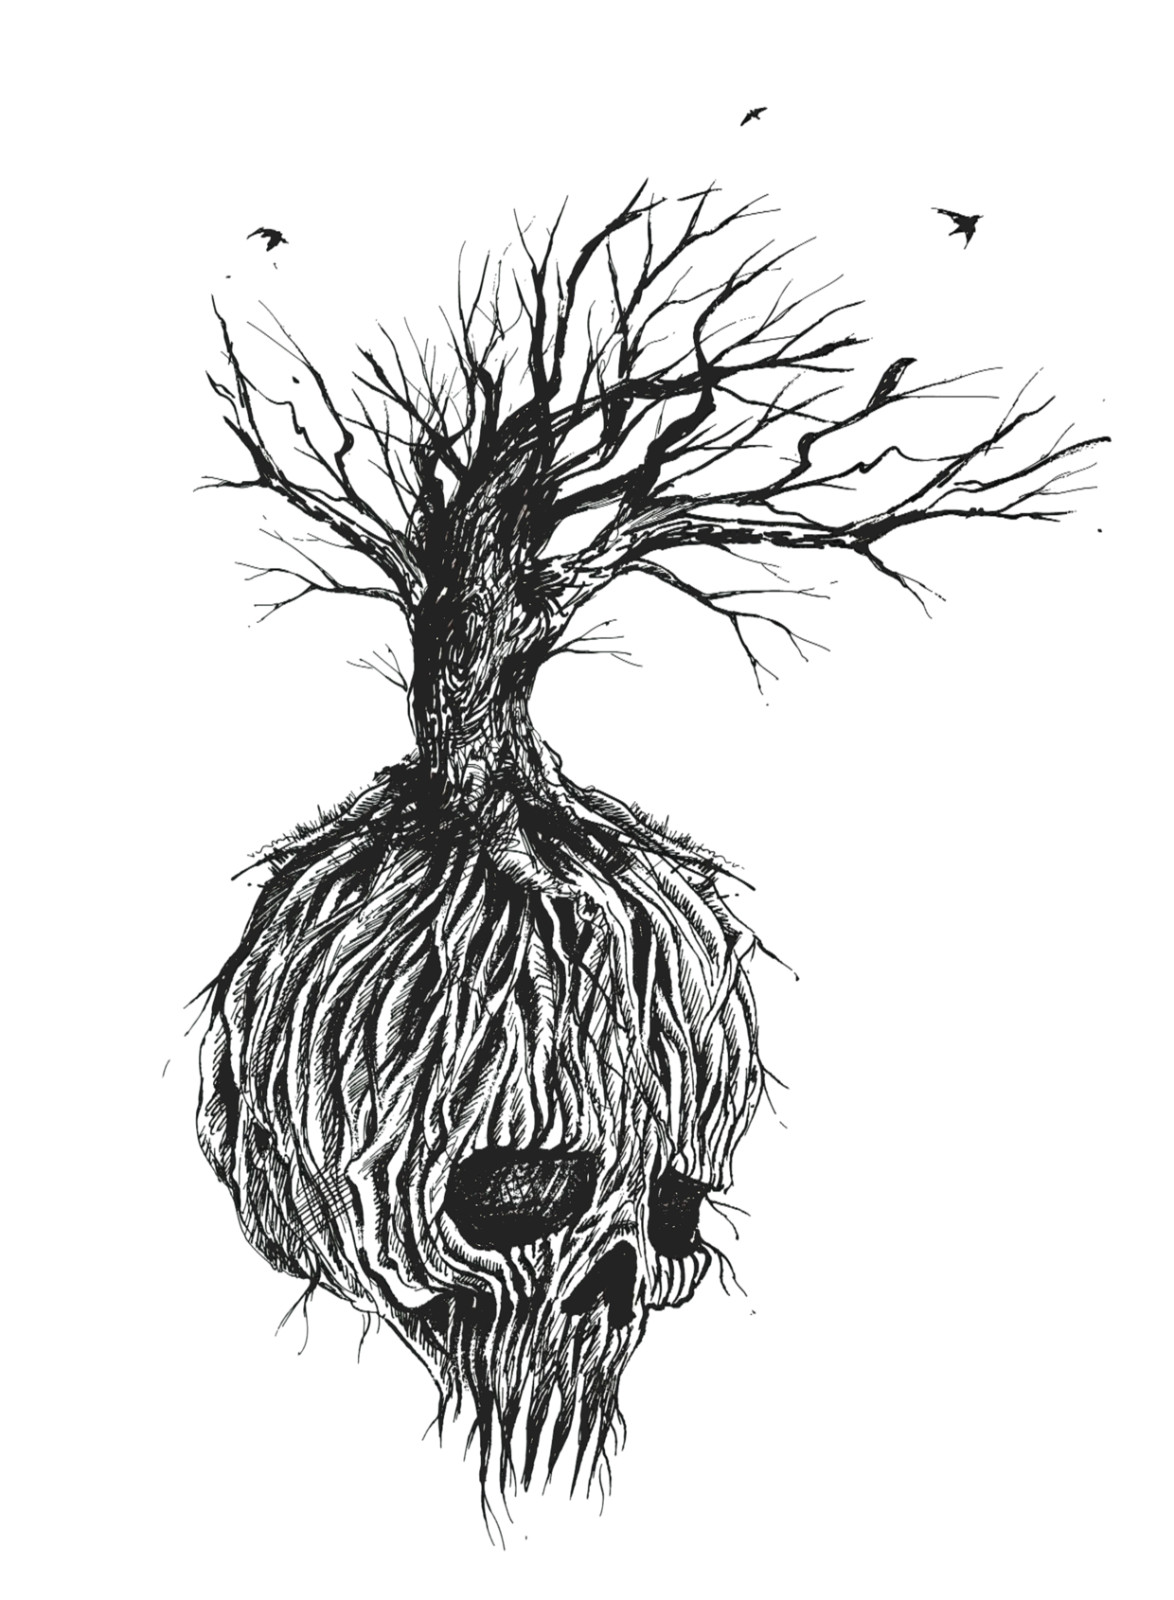
\includegraphics[width=\paperwidth,height=\paperheight]{Images/OGTREE.png}};
    \end{tikzpicture}

    \newcommand{\titleHeader}{\fontsize{60}{70}\selectfont \ringmfamily \color{black}}
    \newcommand{\tituloPosicaoVertical}{3cm}
    \newcommand{\opacityOverlay}{0.10}

    \centering
    \vspace*{\tituloPosicaoVertical}
    {\titleHeader Overgrown Project \par}
    \vspace{1cm}
    {\Large \textbf{João Lucas e Tales Andre} \par}
    \vfill
    {\large Sistema de RPG v1.0 \par}
    \vspace{2cm}
\end{titlepage}
% --- FIM DA CAPA ---

\clearpage
\newgeometry{top=2cm, bottom=2cm, left=1.5cm, right=1.5cm}
\thispagestyle{fancy}

% Sugestão: Use \include para capítulos que começam em nova página
% Use \input para seções que devem continuar na mesma página
\input{Contents/1-introducao}

\midsectiontitle{Atributos do Universo}

Os atributos definem as capacidades essenciais de um personagem, moldando sua força física, agilidade, resistência, percepção, intelecto e conexão com o divino.  
Cada atributo influencia diretamente testes, combates e interações narrativas.

\noindent


% =========================
% DIV
% =========================
\originlink{att:divinity}
\noindent
\hypertarget{target:divinity}{\textbf{\baskerfamily\large DIV — Divinity (Divindade)}}\\
A ligação do jogador com o Pináculo. DIV mede a proximidade do personagem com entidades superiores, deuses e 
forças cósmicas para permitir canalizar suas forças como bem entender. DIV é o único atributo que tem 
limite máximo sendo ele 100 pontos.


% =========================
% MIG
% =========================

\originlink{att:might}
\noindent
\textbf{\baskerfamily\large MIG — Might (Poder)}\\
A força bruta do corpo e da vontade física. MIG governa o dano em combate corpo a corpo baseado em força bruta, 
a capacidade de empunhar armas pesadas e realizar feitos de pura potência, como arrombar portões, erguer estruturas ou 
subjugar inimigos pela força.


% =========================
% GRA
% =========================
\originlink{att:grace}
\noindent
\textbf{\baskerfamily\large GRA — Grace (Graça)}\\
Expressa velocidade, precisão e harmonia de movimento. GRA afeta ataques precisos, esquivas, acrobacias, 
qualquer ação que exija controle corporal refinado. Personagens com alta Graça parecem mover-se como se guiados por mãos divinas.

% =========================
% FOR
% =========================
\originlink{att:fortitude}
\noindent
\textbf{\baskerfamily\large FOR — Fortitude (Fortitude)}\\
A resistência do corpo a todos maléficios externos. FOR define pontos de vida, resistência a doenças, 
venenos e efeitos prolongados. Um personagem com alta Fortitude sobrevive onde outros caem.

% =========================
% WIS
% =========================
\originlink{att:wisdom}
\noindent
\textbf{\baskerfamily\large WIS — Wisdom (Sabedoria)}\\
Representa conhecimento do mundo, entendimento de energias arcanas e o poder de ataque com as mesmas. 
WIS controla o aprendizado, o uso de magias, rituais e a compreensão de fenômenos ocultos. 
Baixa Sabedoria não implica ignorância total, mas limita profundidade e alcance intelectual para assuntos específicos.

% =========================
% SEN
% =========================
\originlink{att:sense}
\noindent
\textbf{\baskerfamily\large SEN — Sense (Sentido)}\\
Representa a percepção aguçada do mundo. SEN engloba testes de observação, intuição e detecção. 
Personagens atentos percebem o que outros ignoram, sons, mentiras, presenças invisíveis.


\titlesection{E Afinal, o que é Divindade em Overgrown?}

Divindade representa o nível de progressão do personagem dentro do sistema de Overgrown. O valor de DIV é sempre igual ao nível do personagem: um personagem de nível 0 possui DIV 0, um personagem de nível 1 possui DIV 1 e assim sucessivamente, até o limite de DIV 100.

Na criação, em \textbf{DIV 0}, o personagem recebe \textbf{5 Pontos de Talento}. A cada novo nível de DIV, recebe mais \textbf{5 Pontos de Talento}. Esse é o único orçamento concedido pela progressão de nível. Portanto:

\[\text{Pontos de Talento totais}=5\times(\text{DIV}+1)\]

Quando a árvore de talentos estiver implementada, esses mesmos pontos poderão ser gastos em qualquer árvore disponível. As árvores conterão tanto \textbf{Nós de Atributo}, que aumentam MIG, GRA, FOR, WIS ou SEN, quanto \textbf{Nós de Habilidade}, que concedem habilidades. Não existe uma reserva separada para atributos e outra para habilidades.

\begin{rpgboxtips}{Modelo Atual sem Árvore}
Enquanto a árvore ainda não estiver implementada, os 5 Pontos de Talento recebidos por DIV são aplicados diretamente em atributos. As habilidades continuam sendo escolhidas individualmente conforme as regras atuais. Quando a árvore for implementada, esse procedimento será substituído pela compra de Nós de Atributo e Nós de Habilidade, sem conceder pontos adicionais retroativos.
\end{rpgboxtips}

Os pontos podem ser guardados, mas um ponto aplicado não pode ser transferido sem um efeito de redistribuição. DIV não recebe esses pontos: ele aumenta junto do nível. Bônus temporários e equipamentos não consomem Pontos de Talento e não cumprem pré-requisitos de valor bruto permanente.
Ao atingir 100 pontos de Divindade, o personagem alcança o limite máximo de conhecimento que uma mente humana 
é capaz de suportar do Pináculo, tornando-se o mais próximo possível de uma entidade divina.

Uma Divindade elevada não impõe, obrigatoriamente, mudanças no comportamento do personagem. 
Contudo, para fins de interpretação (\textit{roleplay}), seus efeitos narrativos podem ser definidos 
de campanha à campanha.

No universo de Overgrown, é possível adquirir divindade de várias formas, 
seja entrando em contato com vestígios restantes de Energia Primordial, estudando conhecimentos divinos ou 
por meio de Combate. Todas as criaturas e seres tem vestígios de divindades, 
essa energia não se dissipa, e matar algo que contem divindade resulta na distribuição i
gualitária dela para quem participar do abate. A tabela abaixo representa o progresso necessário para avançar cada nível de DIV; seus valores não são Pontos de Talento disponíveis para compra.

\begin{rpgboxtips}{Exemplos de Progressão}
Em DIV 0, o personagem possui 5 Pontos de Talento totais. Em DIV 1, possui 10; em DIV 10, 55; em DIV 20, 105; e em DIV 100, 505. Esses valores são o orçamento total recebido pela progressão, antes de bônus externos.
\end{rpgboxtips}

\begin{center}
\renewcommand{\arraystretch}{1.3}
\begin{tabular}{@{} cc @{}}
\toprule
\rowcolor{gray!15} \textbf{Intervalo de Divindade} & \textbf{Progresso por Nível} \\ 
\midrule
01 -- 10 & 10 pts \\
11 -- 20 & 20 pts \\
21 -- 30 & 40 pts \\
31 -- 40 & 80 pts \\
41 -- 50 & 160 pts \\
\midrule
51 -- 60 & 320 pts \\
61 -- 70 & 640 pts \\
71 -- 80 & 1.280 pts \\
81 -- 90 & 2.560 pts \\
91 -- 100 & 5.120 pts \\
\bottomrule
\end{tabular}
\end{center}



\titlesection{Estatísticas dos jogadores}

\subsection*{Modificador de Atributo}

O valor bruto de um atributo determina sua reserva de dados. O \textbf{Modificador de Atributo (MOD)} representa a parcela numérica usada em dano, recuperação e efeitos que pedem explicitamente um modificador. O MOD não é somado a um teste, salvo quando a própria regra mandar fazê-lo.

Para um atributo maior que 0:

\[\text{MOD de Atributo}=\left\lceil\frac{\text{Atributo}}{5}\right\rceil\]

Um atributo 0 possui MOD 0. Assim, atributos de 1--5 possuem MOD 1; 6--10, MOD 2; 11--15, MOD 3; 16--20, MOD 4; e assim sucessivamente. Quando uma regra pedir o maior MOD entre dois atributos, compare os valores brutos e use apenas o MOD do maior; em empate, o resultado é o mesmo e nenhum dado adicional é concedido.

\begin{rpgboxtips}{Valor Bruto e MOD}
Pré-requisitos escritos como \textbf{MIG 15}, \textbf{GRA 10} ou semelhantes usam o valor bruto permanente do atributo. Bônus temporários não cumprem pré-requisitos. Uma expressão como \textbf{MOD de MIG} usa a fórmula acima.
\end{rpgboxtips}

Além dos atributos, jogadores tem algum recursos que são usado durante sua aventura: HP, IEP, Resistência e Esquiva.

HP, Health Points ou Pontos de Vida, representam a vida total do jogador, o quanto de dano ele consegue aguentar e 
é diretamente atrelado a sua \link{att:fortitude}{Fortitude}, cada ponto de Fortitude garante ao jogador 5 de vida e o jogador começa com 10 pontos de vida base. 
Um jogador com 10 de Fortitude terá 60 de vida, excluindo bônus e reduções de vida provenientes da árvore de talentos 
e de itens equipados.

IEP, Impossible Energy Points ou Pontos de Energia Impossível \link{res:null}{(Null)}, 
representa a capacidade do jogador de fazer feitos impossíveis, como usar Magias e Maldições. 
O IEP é diretamente ligado ao \link{att:wisdom}{Wisdom} do jogador, para cada ponto de Wisdom 
garante 5 pontos de IEP ao jogador, e o jogador começa com 10 pontos de IEP base. Um jogador com 10 de Wisdom terá 60 de IEP, excluindo bônus 
e reduções de IEP provenientes da árvore de talentos e de itens equipados.

Resistência define a capacidade do jogador de resistir a ataques, sua classe de armadura. 
É diretamente baseada também na \link{att:fortitude}{Fortitude} 
do jogador. A cada 8 Pontos de Fortitude o jogador ganha 1 ponto de Resistência, tendo 5 pontos base. 
Um jogador com 24 pontos de Fortitude terá 8 de resistência (5 base + 3 vindo dos Atributos), 
excluindo bônus e reduções provenientes da da árvore de talentos e de itens equipados.

\begin{rpgboxtips}{Resistência em Combate}
Resistência é um atributo passivo: ela determina se o ataque ou magia acerta o jogador, mas não reduz o dano recebido. Resistência, Valor de Bloqueio e Redução de Dano são estatísticas diferentes. Um \textbf{Bloqueio} não aumenta a Resistência: ele reduz o dano de um ataque que já acertou, conforme as regras de Armaduras e Proteções.
\end{rpgboxtips}

Esquiva define a proficiência em desviar do jogador. Ela é baseada diretamente ao atributo de \link{att:grace}{Grace}. 
A cada 7 Pontos de Grace, o jogador ganha 1 ponto de Esquiva. Todos os jogadores tem Esquiva base em 5. 
Um jogador com 21 de Grace, tem 8 de esquiva (5 base + 3 dos Pontos de Atributo), 
excluindo bônus e reduções provenientes da árvore de talentos e de itens equipados. 
Caso o rolamento de ataque seja menor que a esquiva do jogador, todo o dano é negado.

\begin{rpgboxtips}{Esquiva em Combate}
Esquivar de um ataque é considerado uma reação, alvos que esquivam perdem a reação na rodada. 
Falhar na esquiva ainda gasta sua reação.
\end{rpgboxtips}

Pontos de Combate é um recurso que representa a capacidade do jogador de realizar ações em combate, como ataques extras ou usar habilidades de combate.
Um jogador com 10 de Grace e 10 de Might, tem 22 pontos de combate (2 base + 10 de Grace + 10 de Might), excluindo bônus e reduções provenientes da árvore de talentos e de itens equipados.



%  Contents/dados_no_overgrown.tex
\midsectiontitle{Dados no Overgrown}

\section*{A Manifestação Numérica}
No universo de \textit{Overgrown}, os dados transcendem a mera casualidade, eles representam a manifestação das capacidades inatas e divinas de um personagem. Cada rolagem é o encontro entre o potencial do aventureiro, os conhecimentos do Pináculo e a pressão do momento presente.

\section*{Os Três Pilares das Rodadas}
Toda interação significativa com o mundo é regida por uma estrutura de três fundamentos que ditam o destino de uma jogada:

\begin{description}
    \item[\ringm{Potencial Inato (Atributos)}:] Refletem a força bruta, agilidade ou a sabedoria divina. No sistema \textit{Overgrown}, o valor do seu atributo não é apenas um bônus, mas o que determina o volume de poder, ou seja, a quantidade de dados, que você pode manifestar em uma ação.
    
    \item[\ringm{Modificadores de Fluxo}:] São as variáveis externas. Bônus provenientes de equipamentos, bênçãos de magias, trilhas da Árvore de Talentos ou vantagens táticas situacionais concedidas pelo mestre.
    
    \item[\ringm{A Resultante Final}:] O ápice da jogada. É a soma do melhor resultado obtido nos dados com os modificadores, definindo se as ações do personagem se empoem sobre a realidade ou se foi superada pelos desafios encontrados.
\end{description}

\section*{Mecânica de Resolução}
O sistema utiliza principalmente o dado de vinte lados (\textbf{d20}) para testes de perícia, ataques e salvaguardas. Dados de outras faces, do \textbf{d2} (Moeda) ao \textbf{d100}, são reservados para calcular o impacto de danos, efeitos de magias e eventos aleatórios do destino.

\subsection*{Ascensão de Atributos}
A maestria em um atributo concede ao personagem uma vantagem grandiosa. A cada \textbf{5 pontos} investidos em um atributo, o aventureiro ganha o direito de arremessar um dado adicional, escolhendo o maior resultado entre eles. Esta progressão não apenas eleva a média dos resultados, mas expande exponencialmente as chances de manifestar um Sucesso Crítico.

\begin{rpgboxtips}{Intervenção Crítica}
Um resultado \textbf{20} natural é um Sucesso Crítico: um acerto garantido que ignora qualquer tentativa de esquiva, podendo ser mitigado apenas por bloqueios. Por outro lado, um \textbf{1} natural é uma Falha Crítica, um erro catastrófico que rompe o fluxo da ação. Lembre-se: cada ataque e magia possui efeitos críticos únicos em suas descrições.
\end{rpgboxtips}

% Tabela de Progressão de Poder
\begin{center}
\renewcommand{\arraystretch}{1.3}
\begin{tabular}{@{} cc @{}}
\toprule
\rowcolor{gray!15} \textbf{\ringm{Magnitude do Atributo}} & \textbf{\ringm{Reserva de Dados (d20)}} \\ 
\midrule
1 -- 5   & 1d20 \\
6 -- 10   & 2d20 \\
11 -- 15 & 3d20 \\
15 -- 20 & 4d20 \\
\textbf{21+} & \textbf{5d20} \\ 
\bottomrule
\end{tabular}
\end{center}

\begin{rpgboxtips}{Além do Limite Mortal}
O limite natural de um aventureiro é a reserva de \textbf{5 dados}. Contudo, aqueles que portam Selos de Divindade ou acessam estados de superiores através de \textbf{Nós Supremos} podem quebrar esta barreira, manifestando reservas de poder que desafiam a compreensão humana. Ter 0 atributos resulta em desvantagem rolando dois dados e pegando o menos.
\end{rpgboxtips}

\begin{comment}
    

\begin{armaCard}{ESPADA DO PINÁCULO}
    \textit{\small Uma lâmina forjada em Verdun, banhada em energia primordial que ressoa com a vontade do portador.}
    
    \vspace{8pt}
    
    % Linha 1 de Atributos
    \attrField{Base Damage}{2D8}
    \attrField{Attribute}{FOR}
    
    \vspace{2pt}
    
    % Linha 2 de Atributos
    \attrField{Multiplier}{2*}
    \attrField{Total DMG}{2D8 + 2*FOR}
    
    \vspace{8pt}
    \overRule
    \vspace{4pt}
    
    % Bloco de MIG, GRA, FOR, WIS, SEN
    \statBox{MIG}{12}
    \statBox{GRA}{08}
    \statBox{FOR}{10}
    \statBox{WIS}{05}
    \statBox{SEN}{06}
    
    \vspace{8pt}
    \overRule
    \vspace{4pt}
    
    % Efeitos Mágicos
    \textbf{\textit{Lâmina de Éter.}} O dano desta arma ignora resistências físicas de seres não-divinos.
    
    \vspace{10pt}
    {\ringmfamily\Large\color{overgrownRed} ACTIONS}
    \overRule
    
    \textbf{\textit{Corte Dimensional (2 Ações).}} O jogador realiza um ataque em área (cone de 3m). Inimigos atingidos devem realizar um teste de \textbf{GRA} ou sofrerão o dano total da arma.
    
\end{armaCard}
\end{comment}
% Contents/lutas_e_combates.tex
\midsectiontitle{Combate em OverGrown}

\titlesection{A Rolagem de Iniciativa}

No \textit{Overgrown}, o combate não é um mero caos, mas uma sequência de movimentos calculados onde a velocidade e a percepção ditam a sobrevivência. Quando as lâminas se cruzam, a ordem das ações é determinada pelo teste de \link{att:grace}{Grace} somado ao Modificador de Iniciativa. Este valor representa a prontidão do aventureiro em resposta à ameaça iminente.

\begin{rpgboxtips}{Rolagem de Iniciativa}
A iniciativa é rolada no início de cada combate com base em \link{att:grace}{Grace}. Aquele que obtiver o maior resultado age primeiro, seguido pelos demais em ordem decrescente. Em caso de empate, o personagem com maior \link{att:grace}{Grace} age primeiro; persistindo o empate, o Mestre decide ou permite nova rolagem.
\end{rpgboxtips}

Aqueles que se destacam agem primeiro, estabelecendo o ritmo do confronto, seguidos pelos demais em ordem decrescente de seus resultados.

\begin{rpgboxtips}{A Estratégia do Atraso}
Um combatente astuto sabe que nem sempre golpear primeiro é a melhor escolha. Você pode optar por \textbf{atrasar sua ação}, aguardando o momento exato em que um aliado abre uma brecha ou um inimigo se expõe. Ao fazer isso, sua posição na ordem de combate é permanentemente redefinida para este novo marco até o desfecho da cena.
\end{rpgboxtips}

\titlesection{O Fluxo do Tempo e Ações}

O tempo em combate é uma percepção fragmentada. Cada turno condensa entre 0,5 e 6 segundos, onde decisões devem ser tomadas com precisão antes de serem enunciadas. Sob o olhar do mestre, o impossível pode ser tentado, mas apenas o que for coerente com o fluxo temporal será executado.

\subsection*{A Hierarquia das Ações}

A economia de combate em \textit{Overgrown} é baseada na versatilidade. Cada combatente possui uma quantidade limitada de energia e pontos de combate que se traduz em quatro tipos de ações: \textbf{Padrão (ou Completa)}, \textbf{Movimento}, \textbf{Livre} e \textbf{Reação}.

A maestria reside na conversão de esforços. O sistema permite que o jogador sacrifique uma ação de maior complexidade para realizar múltiplas tarefas mais simples.

\begin{itemize}
    \item \textbf{Ação Padrão:} O núcleo do seu turno. Usada para atacar ou usar magias. Pode ser convertida em uma ação de Movimento, Livre ou em uma Reação adicional.
    \item \textbf{Ação de Movimento:} Utilizada para reposicionamento. Pode ser convertida em uma ação Livre.
    \item \textbf{Ação Livre:} Ações rápidas ou frases curtas. Não pode ser convertida.
    \item \textbf{Reação:} Uma resposta instintiva fora do seu turno (1 por rodada). Não pode ser convertida ou trocada. Esquivar de um ataque, bloquear, contra-atacar e interromper conjurações são exemplos de Reações.
\end{itemize}

\begin{rpgboxtips}{Conversão em Reação}
Uma Ação Padrão só pode ser convertida em Reação durante o próprio turno. A Reação adicional fica disponível até o início do próximo turno do personagem e desaparece caso não seja usada. Ela se soma à Reação normal da rodada, permitindo no máximo duas Reações nesse intervalo, salvo quando uma habilidade declarar outro limite. A conversão não pode ser feita retroativamente depois que já ocorreu.
\end{rpgboxtips}

\titlesection{Nível de Ameaça e Precisão}

\subsection*{Teste de Ataque}

Para resolver um ataque, role a reserva de d20 determinada pelo atributo indicado pela arma, magia ou habilidade e conserve o maior resultado. Em seguida, some a Perícia de Combate apropriada e quaisquer bônus ou penalidades que declarem afetar o teste de ataque:

\begin{itemize}
    \item \textbf{Luta:} ataques corpo a corpo, incluindo armas brancas e ataques desarmados.
    \item \textbf{Pontaria:} ataques com armas de longo alcance, mesmo quando a arma utilizar MIG em vez de GRA para formar sua reserva.
    \item \textbf{Arcanismo:} ataques de magias e ataques básicos de armas mágicas que utilizem WIS.
\end{itemize}

\[\text{Resultado de Ataque}=\text{maior d20 da reserva}+\text{Perícia de Combate}+\text{bônus e penalidades de acerto}\]

O ataque acerta quando seu resultado iguala ou supera a defesa aplicável do alvo. Um 20 natural continua sendo um acerto crítico garantido e um 1 natural continua sendo uma falha crítica, independentemente do total após os bônus.

O \textbf{MOD de Atributo não participa do teste de ataque}. Expressões como \textbf{MOD de MIG}, \textbf{MOD de GRA}, \textbf{MOD de WIS} ou \textbf{MOD de SEN} presentes na ficha da arma ou da magia são somadas somente ao dano, depois de confirmar o acerto. Por exemplo, uma arma corpo a corpo com dano \textbf{2D6 + MOD de MIG} testa o acerto usando a reserva indicada + Luta; ao acertar, causa 2D6 + MOD de MIG. Uma arma física à distância testa com Pontaria e acrescenta MOD de SEN ao dano.

\subsection*{Regra unificada de ataques à distância}
Arcos, bestas, pistolas, rifles, espingardas e demais armas físicas de longo alcance usam \textbf{Pontaria} no teste de ataque e \textbf{MOD de SEN} no dano. Exemplo: um Rifle de Precisão causa \textbf{2D10 + MOD de SEN}. Uma arma híbrida usa SEN apenas no modo à distância; uma Lança arremessada usa SEN, mas empunhada em corpo a corpo mantém MIG. Magias projetadas e focos arcanos continuam usando a regra da magia e seu atributo mágico.

\originlink{stats:crit}
No mundo de \textit{Overgrown}, o \textbf{Nível de Ameaça} descreve o potencial do aventureiro de encontrar brechas na defesa inimiga e atingir pontos vitais com precisão absoluta.

Por padrão, um Crítico ocorre ao obter um \textbf{20 natural} nos dados. Entretanto, através de armas específicas e do avanço nos conhecimentos da \textbf{Árvore de Talentos}, este limiar de precisão pode ser reduzido. Um aventureiro de elite pode expandir sua margem de ameaça para resultados como 19, 18 ou até menores, tornando cada golpe uma ameaça potencialmente letal.

\begin{rpgboxtips}{Nós de Agilidade}
Não ignore a Árvore de Talentos durante seus treinos. Existem \textbf{Nós de Estatísticas} e \textbf{Nós Supremos} focados especificamente em quebrar as regras de tempo, permitindo que ações de movimento concedam bônus extras ou que reações sejam recuperadas mais rapidamente.
\end{rpgboxtips}

Um aventureiro por padrão tem 7 unidades de movimento, mas para cada 10 pontos de Grace, ele ganha 1 unidade adicional. Assim, um personagem com 25 de Graça teria 9 unidades de movimento, permitindo-lhe se deslocar mais rapidamente pelo campo de batalha e alcançar posições estratégicas com maior facilidade.

\titlesection{Cobertura}

Obstáculos físicos entre o atirador e o alvo concedem proteção. Em \textit{Overgrown}, a cobertura é classificada em dois graus:

\begin{description}
    \item[\ringm{Cobertura Parcial}:] O alvo está protegido por um obstáculo que cobre \textbf{metade ou menos} de seu corpo (parapeito, pilar, canto de parede). O atirador sofre \textbf{$-$5 de acerto} nos ataques à distância contra esse alvo. O alvo ainda pode ser atingido normalmente caso o ataque supere essa penalidade.
    \item[\ringm{Cobertura Total}:] O alvo está completamente atrás de um obstáculo sólido, sem linha de visão direta. Ataques à distância comuns são \textbf{impossíveis} contra alvos em cobertura total. Apenas habilidades específicas (como \textit{Tiro Ricochete} ou \textit{Tiro em Curva}) ou magias de área permitem contornar este impedimento.
\end{description}

\begin{rpgboxtips}{Cobertura e Corpo a Corpo}
Cobertura não oferece proteção contra ataques corpo a corpo. Um inimigo que atravessar o obstáculo ou alcançar o alvo fisicamente ignora qualquer bônus de cobertura.
\end{rpgboxtips}

\titlesection{Canalização Mágica com Armas}

Certas armas possuem afinidade com energias arcanas e podem ser usadas como catalisadores para magias, transformando projéteis comuns em veículos de destruição mágica.

\begin{description}
    \item[\ringm{Arcos}:] Arcos são excelentes condutores de energia primordial. Ao canalizar uma magia através de um arco, o conjurador dispara a magia como se fosse uma flecha. O ataque utiliza o \link{stats:crit}{Nível de Ameaça} do arco e seus bônus de distância. A magia herda o tipo de dano definido pelo conjurador. Por continuar sendo uma magia, o teste soma \textbf{Arcanismo} e mantém \textbf{Wisdom}; não se converte em um ataque físico de Sense.
    \item[\ringm{Armas de Fogo}:] Por serem forjadas com gravuras de combustão rúnica focadas em dano físico bruto, armas de fogo \textbf{não podem ser usadas como canalizadores mágicos}. Tentar fazê-lo dissipa a magia sem efeito e gasta o IEP normalmente.
\end{description}

\begin{rpgboxtips}{Flechas Especiais e Magia}
Flechas de Aetherium e Rúnicas amplificam ainda mais magias canalizadas. O dano extra da flecha é adicionado ao dano da magia disparada, tornando a combinação de arqueria e arcanismo uma especialização poderosa.
\end{rpgboxtips}

%\input{Contents/arvore_de_habilidade_e_talentos}
% Contents/inventario_e_carga.tex
\midsectiontitle{Inventário e Carga}

\titlesection{O Fardo do Aventureiro}

No universo de \textit{Overgrown}, cada objeto tem sua propria unidade de peso. A capacidade de carga básica de um indivíduo é de \textbf{10 unidades}, representando o limite de volume e peso que pode ser manejado sem comprometer a mobilidade.

Este limite é ampliado pela força física do aventureiro: para cada ponto investido em \link{att:might}{Might (Poder)}, o aventureiro expande sua capacidade de carga em \textbf{1 unidade}. Embora o Pináculo não imponha um limite absoluto para o que se pode carregar, o excesso de peso além da capacidade total resultará em penalidades severas de movimento e ações. Pra cada 1 unidade de Peso acima da carga do aventureiro, este perde 5 de movimento.

\begin{rpgboxtips}{Bonificações Temporárias}
Bônus temporários de atributos ou estados de fúria momentânea não expandem sua capacidade de carga máxima. Apenas melhorias permanentes provenientes da \textbf{Árvore de Talentos} ou artefatos  alteram o limite de transporte do personagem.
\end{rpgboxtips}

\titlesection{Armamentos e Projéteis}

O manejo de recursos é vital para a sobrevivência. Armas que dependem de munição seguem regras distintas baseadas em sua natureza.

\subsection*{A Ciência da Pólvora}
Armas de fogo, como pistolas, rifles e fuzis são maravilhas da engenharia rúnica. Elas não são meramente mecânicas, mas forjadas com gravuras que estabilizam a combustão da \textbf{Munição de Pólvora}. 
\begin{itemize}
    \item \textbf{Consumo:} Cada unidade de munição de pólvora é preparada para sustentar o aventureiro por uma \textbf{Cena} inteira de combate.
    \item \textbf{Carga:} Cada suprimento de cena pesa baseado no tipo de arma.
    \item \textbf{Natureza:} Embora sejam armas mágicas por fabricação, elas são focadas na entrega de dano físico bruto e, por regra geral, não servem como canalizadores para magias ativas.
\end{itemize}

\subsection*{A Arte do Arco e Flecha}
Diferente das armas de fogo, os arcos são extensões da alma do arqueiro e excelentes condutores de energia primordial. 
\begin{itemize}
    \item \textbf{Consumo:} Flechas básicas não são contabilizadas por combate, mas sim por \textbf{Aventura}, tendo que ser repostas em períodos de descanso ou em mercadores.
    \item \textbf{Carga:} Cada suprimento de flechas pesa 1 unidade, independentemente do tipo, mas o peso total pode variar conforme a qualidade e material da flecha.
    \item \textbf{Canalização:} Arcos podem ser usados como canalizadores mágicos, permitindo disparar feitiços como se fossem flechas. Nesta forma, a magia herda as propriedades do arco, como o \link{stats:crit}{Nível de Ameaça (Crítico)} e bônus de distância.
\end{itemize}

\begin{center}
\renewcommand{\arraystretch}{1.2}
\begin{tabular}{lcc}
\toprule
\rowcolor{gray!15} \textbf{\ringm{Tipo de Projétil}} & \textbf{\ringm{Peso de Carga}} & \textbf{\ringm{Dano Extra}} \\ 
\midrule
Flechas de Ferro ou Aço & 1 & --- \\
Flechas Rúnicas (Engravadas) & 3 & +1d6 Perfurante \\
Flechas de Aetherium (Vastidrum) & 5 & +1d8 Perfurante \\
\bottomrule
\end{tabular}
\end{center}

\titlesection{Proteção e Utilitários}

As armaduras são classificadas por sua densidade e material, afetando diretamente o fardo do usuário. Armaduras especiais podem ter pesos alterados conforme suas especificações técnicas.

\begin{description}
    \item[\ringm{Pano (Peso 2)}:] Vestes leves geralmente usada por magos.
    \item[\ringm{Couro (Peso 4)}:] Proteção flexível e leve.
    \item[\ringm{Malha (Peso 7)}:] O equilíbrio entre defesa e peso.
    \item[\ringm{Metal (Peso 10)}:] Proteção pesada para a linha de frente.
    \item[\ringm{Placas (Peso 15)}:] A fortaleza intransponível do guerreiro.
\end{description}

Poções para uso rapido são guardadas em um cinto de poções do aventureiro, que tem capacidade para 5 frascos. Cada frasco pesa 0.4 unidade, totalizando 2 unidades. Existem cintos de poções maiores, no entanto devem ser adquiridos ou comprados.
Poções no cinto de poção podem ser tomadas como ação livre, e deve ser reabastecido durante descanso ou em ação padrão durante o combate. Poções guardadas no inventário não podem ser usadas durante o combate, e devem ser transferidas para o cinto de poções para serem utilizadas.

\midsectiontitle{Armas e Armaduras}

Em \textit{Overgrown}, cada arma é uma escolha de identidade.
Não existem regras para ditar quantas armas o aventureiro pode carregar ou quando utilizá-las, estar preparado
é parte do valor de sobreviver no Pináculo.

\begin{rpgboxtips}{Requisitos de Armas}
Cada arma possui um ou mais requisitos de atributos permanentes. Esses requisitos não dependem de DIV e podem ser cumpridos em qualquer nível. Bônus temporários, magias e estados não contam para esse fim.

Um personagem que não cumpra todos os requisitos ainda pode empunhar e atacar com a arma. Enquanto estiver empunhando ou utilizando essa arma, sofre \textbf{$-$10 em todos os testes que realizar}, mesmo quando o teste não estiver diretamente relacionado à arma. A penalidade termina assim que a arma deixa de ser empunhada ou utilizada. Rolagens de dano não são testes e não recebem essa penalidade.
\end{rpgboxtips}

\begin{rpgboxtips}{Configurações de Empunhadura Dupla}
Certos pares de armas formam uma \textbf{Configuração de Empunhadura Dupla}, apresentada em perfil próprio. Para usar esse perfil, o personagem deve empunhar uma cópia válida da arma em cada mão e cumprir o requisito da configuração.

Ao realizar um ataque, declare se está usando o perfil individual de uma das armas ou o perfil da configuração. O perfil de Empunhadura Dupla substitui o dano, a Ameaça e as Propriedades Especiais das armas individuais durante toda a ação. Benefícios dos dois perfis individuais não se acumulam com o perfil duplo. Ataques separados concedidos por uma configuração contam para o limite geral de ataques adicionais e não geram novos ataques extras. Uma configuração não pode usar Golpe Duplo, Disparo Duplo, Ataque Secundário ou outra fonte de ataque adicional na mesma ação.
\end{rpgboxtips}

% ==============================================================================
\titlesection{Armas Corpo a Corpo}
% ==============================================================================

\renewcommand{\tabularxcolumn}[1]{m{#1}}
\setlength{\extrarowheight}{3pt}
\renewcommand{\arraystretch}{1.2}
\begin{tabularx}{\textwidth}{|>{\columncolor{white}\centering\arraybackslash}m{0.18\textwidth}|>{\columncolor{white}\centering\arraybackslash}m{0.08\textwidth}|>{\columncolor{white}\centering\arraybackslash}m{0.06\textwidth}|>{\columncolor{white}\centering\arraybackslash}m{0.13\textwidth}|>{\columncolor{white}\centering\arraybackslash}m{0.12\textwidth}|>{\columncolor{white}\centering\arraybackslash}X|}
    \hline
    \multicolumn{1}{|c|}{\textbf{\ringm{Nome}}} &
    \multicolumn{1}{c|}{\textbf{\ringm{Ameaça}}} &
    \multicolumn{1}{c|}{\textbf{\ringm{Peso}}} &
    \multicolumn{1}{c|}{\textbf{\ringm{Dano Base}}} &
    \multicolumn{1}{c|}{\textbf{\ringm{Requisito}}} &
    \multicolumn{1}{c|}{\textbf{\ringm{Propriedade Especial}}} \\
    \hline
    Adaga & 18 & 1 & 1D6 + MOD de GRA & GRA 3 & \textbf{Assassin:} Contra um alvo Desprevenido, o primeiro acerto da cena aplica \link{status:ardiloso}{Sangramento Ardiloso}. \\
    \hline
    Alabarda & 19 & 5 & 2D8 + MOD de MIG & MIG 10 e SEN 5 & \textbf{Halberdier:} Alterne entre dano cortante e perfurante. Inimigos que avançarem a 2 unidades sofrem ataque de oportunidade. Acertos críticos aplicam \link{status:brutal}{Sangramento Brutal}. \\
    \hline
    Bo & 20 & 3 & 2D6 + MOD de MIG & MIG 3 e GRA 3 & \textbf{Monk:} Acertos críticos aplicam \link{status:concussionado}{Concussão}. Acertos comuns concedem +1 Esquiva até seu próximo turno (acumulável até +3). \\
    \hline
    Clava & 20 & 2 & 1D8 + MOD de MIG & MIG 2 & \textbf{Bruta:} Arma simples de impacto. Acertos críticos aplicam \link{status:concussionado}{Concussão} e \link{status:brutal}{Sangramento Brutal}. \\
    \hline
    Escudo & 20 & 3 & 1D6 + MOD de MIG & FOR 3 & \textbf{Guardian:} Ocupa uma mão e adiciona \textbf{+5 ao Valor de Bloqueio}. Apenas um escudo pode contribuir para cada Bloqueio. \\
    \hline
    Espada de Duas Mãos & 20 & 4 & 3D6 + MOD de MIG & MIG 10 e FOR 5 & \textbf{Guerreiro:} Adiciona \textbf{+3 ao Valor de Bloqueio}. Quando um alvo bloquear um ataque desta arma, reduza o Valor de Bloqueio total dele à metade, arredondando para baixo. \\
    \hline
    Espada de Uma Mão & 19 & 2 & 2D6 + MOD de MIG & MIG 5 & \textbf{Warden:} Use escudo sem penalidade de carga. \\
    \hline
    Lança & 19 & 3 & 2D8 + MOD de MIG & MIG 7 e SEN 3 & \textbf{Lancer:} Inimigos que avançarem a 1 unidade sofrem ataque de oportunidade. Pode ser arremessada (4 unidades), causando metade do dano. \\
    \hline
    Machado de Uma Mão & 19 & 3 & 2D6 + MOD de MIG & MIG 5 & \textbf{BloodLetter:} Acertos críticos aplicam \link{status:brutal}{Sangramento Brutal}. \\
    \hline
\end{tabularx}

\vspace{4pt}
\renewcommand{\tabularxcolumn}[1]{m{#1}}
\setlength{\extrarowheight}{3pt}
\renewcommand{\arraystretch}{1.2}
\begin{tabularx}{\textwidth}{|>{\columncolor{white}\centering\arraybackslash}m{0.18\textwidth}|>{\columncolor{white}\centering\arraybackslash}m{0.08\textwidth}|>{\columncolor{white}\centering\arraybackslash}m{0.06\textwidth}|>{\columncolor{white}\centering\arraybackslash}m{0.13\textwidth}|>{\columncolor{white}\centering\arraybackslash}m{0.12\textwidth}|>{\columncolor{white}\centering\arraybackslash}X|}
    \hline
    \multicolumn{1}{|c|}{\textbf{\ringm{Nome}}} &
    \multicolumn{1}{c|}{\textbf{\ringm{Ameaça}}} &
    \multicolumn{1}{c|}{\textbf{\ringm{Peso}}} &
    \multicolumn{1}{c|}{\textbf{\ringm{Dano Base}}} &
    \multicolumn{1}{c|}{\textbf{\ringm{Requisito}}} &
    \multicolumn{1}{c|}{\textbf{\ringm{Propriedade Especial}}} \\
    \hline
    Machado de Duas Mãos & 20 & 7 & 3D8 + MOD de MIG & MIG 12 e FOR 5 & \textbf{Berserker:} Todo acerto aplica \link{status:brutal}{Sangramento Brutal}. Com armadura leve ou sem armadura, causa 2D6 adicional. \\
    \hline
    Maça de Uma Mão & 19 & 3 & 2D6 + MOD de MIG & MIG 5 & \textbf{Crusader:} Com escudo, causa 1D8 adicional. Em acertos críticos, reduza em 2 o Valor de Bloqueio usado contra o ataque, até o mínimo de 0. \\
    \hline
    Maça de Duas Mãos & 20 & 6 & 2D8 + 1D6 + MOD de MIG & MIG 10 e FOR 5 & \textbf{Legionary:} Acertos críticos aplicam \link{status:atordoado}{Atordoado} por 1 turno. Ataques reduzem Resistência do alvo em 1 (máx. $-$5). \\
    \hline
    Martelo de Uma Mão & 19 & 3 & 2D6 + MOD de MIG & MIG 6 e FOR 3 & \textbf{Templar:} Com escudo, causa 1D8 adicional. Acertos aplicam \link{status:brutal}{Sangramento Brutal}. \\
    \hline
    Martelo de Duas Mãos & 20 & 6 & 2D10 + MOD de MIG & MIG 12 e FOR 5 & \textbf{Avenger:} Adiciona \textbf{+3 ao Valor de Bloqueio}. Acertos críticos aplicam \link{status:brutal}{Sangramento Brutal} e \link{status:concussionado}{Concussão} simultaneamente. \\
    \hline
    Rapieira & 18 & 2 & 2D6 + MOD de GRA & GRA 8 e SEN 3 & \textbf{Duelist:} Reduza em 2 PC o custo de Ataque Secundário com esta arma, até o mínimo de 3 PC. Se o alvo errar um ataque contra você, ganhe \textbf{Vantagem} no próximo ataque contra ele. \\
    \hline
    Soqueiras & 19 & 1 & 1D6 + MOD de GRA & GRA 8 e MIG 3 & \textbf{Pugilist:} Para cada 5 MOD de GRA, realize um ataque adicional ao usar uma Ação Padrão para atacar com as Soqueiras. Cada ataque adicional causa apenas 1D6, sem MOD ou dano adicional, não pode resultar em crítico, não ativa efeitos ao acertar e não gera outros ataques. Esta é uma exceção expressa ao limite geral de um ataque adicional. Ao avançar em direção a um inimigo para atacar, você \textbf{não provoca ataques de oportunidade} nesse deslocamento. \\
    \hline
    Tonfa & 19 & 2 & 1D8 + MOD de MIG & GRA 5 e FOR 5 & \textbf{Enforcer:} Quando seu Bloqueio reduzir ao menos 1 ponto de dano de um ataque corpo a corpo, receba +1 VB até o início do próximo turno. \\
    \hline
\end{tabularx}

% ==============================================================================
\titlesection{Armas de Longo Alcance}
% ==============================================================================

\vspace{4pt}
\renewcommand{\tabularxcolumn}[1]{m{#1}}
\setlength{\extrarowheight}{3pt}
\renewcommand{\arraystretch}{1.2}
\begin{tabularx}{\textwidth}{|>{\columncolor{white}\centering\arraybackslash}m{0.18\textwidth}|>{\columncolor{white}\centering\arraybackslash}m{0.08\textwidth}|>{\columncolor{white}\centering\arraybackslash}m{0.06\textwidth}|>{\columncolor{white}\centering\arraybackslash}m{0.13\textwidth}|>{\columncolor{white}\centering\arraybackslash}m{0.12\textwidth}|>{\columncolor{white}\centering\arraybackslash}X|}
    \hline
    \multicolumn{1}{|c|}{\textbf{\ringm{Nome}}} &
    \multicolumn{1}{c|}{\textbf{\ringm{Ameaça}}} &
    \multicolumn{1}{c|}{\textbf{\ringm{Peso}}} &
    \multicolumn{1}{c|}{\textbf{\ringm{Dano Base}}} &
    \multicolumn{1}{c|}{\textbf{\ringm{Requisito}}} &
    \multicolumn{1}{c|}{\textbf{\ringm{Propriedade Especial}}} \\
    \hline
    Arco Composto & 19 & 5 & 2D8 + MOD de GRA & GRA 8, MIG 5 e SEN 3 & \textbf{Hunter:} Ataques acima de 20 unidades têm Vantagem e +1D6. Pode canalizar magias como flechas. \\
    \hline
    Arco Leve & 20 & 1 & 1D8 + MOD de GRA & GRA 3 & \textbf{Scout:} Oculto ou primeiro a atacar, causa 1D8 extra. Pode ser empunhado e guardado como ação livre. \\
    \hline
    Arco Recurvo & 19 & 3 & 2D6 + MOD de GRA & GRA 6 e SEN 3 & \textbf{Ranger:} Em terreno elevado, causa 1D6 extra. Pode canalizar magias como flechas. \\
    \hline
    Besta Leve & 19 & 3 & 2D6 + MOD de GRA & GRA 3 e SEN 2 & \textbf{Pathfinder:} Seu mecanismo rúnico permite disparar sem gastar ação para recarregar. \\
    \hline
    Besta Pesada & 20 & 5 & 3D6 + MOD de GRA & GRA 6 e SEN 5 & \textbf{Marksman:} Marque um alvo no início do combate; ataques contra ele causam 1D8 extra. Exige ação de movimento para recarregar. \\
    \hline
    Bola de Cristal & 20 & 2 & 1D6 + MOD de WIS & WIS 8 e SEN 3 & \textbf{Channeler:} Adiciona metade do MOD de WIS (arredondado acima) aos testes de ataque mágico e o MOD de WIS completo ao dano de magias. \\
    \hline
    Bucaneira & 20 & 7 & 3D6 + MOD de MIG & MIG 10 e FOR 7 & \textbf{Buccaneer:} Acertos críticos ignoram o Valor de Bloqueio da armadura do alvo, mas não o bônus de escudos ou armas, e aplicam \link{status:brutal}{Sangramento Brutal}. Exige ação de movimento para recarregar. \\
    \hline
    Cajado & 20 & 3 & 2D6 + MOD de WIS & WIS 3 & \textbf{Arcanist:} Ao conjurar magias, gaste 10 IEP para aumentar o dano em 1D10. Pode ser usado em corpo a corpo sem penalidade. \\
    \hline
\end{tabularx}

\vspace{4pt}
\renewcommand{\tabularxcolumn}[1]{m{#1}}
\setlength{\extrarowheight}{3pt}
\renewcommand{\arraystretch}{1.2}
\begin{tabularx}{\textwidth}{|>{\columncolor{white}\centering\arraybackslash}m{0.18\textwidth}|>{\columncolor{white}\centering\arraybackslash}m{0.08\textwidth}|>{\columncolor{white}\centering\arraybackslash}m{0.06\textwidth}|>{\columncolor{white}\centering\arraybackslash}m{0.13\textwidth}|>{\columncolor{white}\centering\arraybackslash}m{0.12\textwidth}|>{\columncolor{white}\centering\arraybackslash}X|}
    \hline
    \multicolumn{1}{|c|}{\textbf{\ringm{Nome}}} &
    \multicolumn{1}{c|}{\textbf{\ringm{Ameaça}}} &
    \multicolumn{1}{c|}{\textbf{\ringm{Peso}}} &
    \multicolumn{1}{c|}{\textbf{\ringm{Dano Base}}} &
    \multicolumn{1}{c|}{\textbf{\ringm{Requisito}}} &
    \multicolumn{1}{c|}{\textbf{\ringm{Propriedade Especial}}} \\
    \hline
    Espingarda de Caça & 19 & 4 & 2D8 + MOD de GRA & GRA 7, MIG 5 e SEN 3 & \textbf{Trapper:} Use Mira Focada como ação livre, sem gastar PC. Até 5 unidades, causa 1D6 extra. Exige ação de movimento para recarregar. \\
    \hline
    Grimório & 19 & 2 & 1D8 + MOD de WIS & WIS 10 e SEN 5 & \textbf{Archmage:} Durante um Descanso Pleno, armazene no Grimório uma magia cuja fórmula esteja disponível ao personagem. Apenas uma magia pode ficar armazenada por vez; armazenar outra substitui a anterior. A magia armazenada pode ser conjurada mesmo fora das escolhas atuais do personagem, mas cada conjuração paga seu custo de IEP normalmente. Se estiver fora das escolhas atuais, seu custo de IEP é dobrado. O Grimório nunca elimina o custo da magia. \\
    \hline
    Pistola & 18 & 2 & 2D6 + MOD de GRA & GRA 5 e SEN 3 & \textbf{Gunslinger:} Recarregar a pistola exige uma ação de Movimento. \\
    \hline
    Rifle de Precisão & 19 & 8 & 2D10 + MOD de GRA & GRA 10 e SEN 10 & \textbf{Deadeye:} Acertos críticos causam 1D10 extra e ignoram o Valor de Bloqueio da armadura do alvo, mas não o bônus de escudos ou armas. Recarregar exige ação padrão completa. Desvantagem contra alvos a menos de 5 unidades. \\
    \hline
    Varinha & 19 & 1 & 1D8 + MOD de WIS & WIS 3 e SEN 2 & \textbf{Sorcerer:} Ataque básico causa Dano Mágico sem consumir IEP. Quando esse ataque causa ao menos 1 ponto de dano a um alvo vivo, aliado ou inimigo, recupere 1D4 IEP. Um mesmo alvo só pode alimentar esta recuperação uma vez por rodada, e a recuperação não pode elevar o IEP acima do máximo. Construtos, objetos, cadáveres e alvos sem vida não ativam o efeito. \\
    \hline
\end{tabularx}

% ==============================================================================
\titlesection{Configurações de Empunhadura Dupla}
% ==============================================================================

Os perfis abaixo são tratados como armas próprias durante a ação em que forem usados. O peso indicado é o peso total do par. Salvo indicação contrária, somente o primeiro ataque da configuração soma MOD ao dano.

\vspace{4pt}
\begin{tabularx}{\textwidth}{|>{\columncolor{white}\centering\arraybackslash}m{0.19\textwidth}|>{\columncolor{white}\centering\arraybackslash}m{0.08\textwidth}|>{\columncolor{white}\centering\arraybackslash}m{0.06\textwidth}|>{\columncolor{white}\centering\arraybackslash}m{0.14\textwidth}|>{\columncolor{white}\centering\arraybackslash}m{0.13\textwidth}|>{\columncolor{white}\centering\arraybackslash}X|}
    \hline
    \multicolumn{1}{|c|}{\textbf{\ringm{Configuração}}} &
    \multicolumn{1}{c|}{\textbf{\ringm{Ameaça}}} &
    \multicolumn{1}{c|}{\textbf{\ringm{Peso}}} &
    \multicolumn{1}{c|}{\textbf{\ringm{Dano Base}}} &
    \multicolumn{1}{c|}{\textbf{\ringm{Requisito}}} &
    \multicolumn{1}{c|}{\textbf{\ringm{Propriedade Especial}}} \\
    \hline
    Adagas Gêmeas & 19 & 2 & Dois ataques de 1D6 & GRA 8 & \textbf{Twin Assassin:} Os dois ataques sofrem apenas $-$1 de acerto. Se ambos acertarem o mesmo alvo, aplique uma carga de \link{status:ardiloso}{Sangramento Ardiloso}. Aplique no máximo uma carga por ação. \\
    \hline
    Espadas Gêmeas & 19 & 4 & Dois ataques de 1D8 & MIG 7 e GRA 5 & \textbf{Twin Warden:} Os dois ataques sofrem $-$2 de acerto. Se ambos acertarem o mesmo alvo, cause +1D6 de dano após resolver o segundo ataque. \\
    \hline
    Machados Gêmeos & 20 & 6 & Dois ataques de 1D8 & MIG 8 e GRA 5 & \textbf{Twin BloodLetter:} Os dois ataques sofrem $-$2 de acerto. Se ambos causarem dano ao mesmo alvo, o segundo aplica \link{status:brutal}{Sangramento Brutal}. \\
    \hline
    Tonfas Gêmeas & 19 & 4 & 2D6 + MOD de MIG & GRA 7 e FOR 5 & \textbf{Twin Enforcer:} Adicione +3 VB. Uma vez por rodada, quando um Bloqueio reduzir dano de ataque corpo a corpo, gaste 2 PC para contra-atacar imediatamente. Esse ataque não exige nova Reação e não gera ataques adicionais. \\
    \hline
    Bestas Leves Gêmeas & 20 & 6 & Dois ataques de 1D8 & GRA 7 e SEN 5 & \textbf{Twin Pathfinder:} Os ataques sofrem $-$2 de acerto e podem escolher alvos diferentes. Os mecanismos rúnicos independentes não exigem ação de recarga. \\
    \hline
    Pistolas Gêmeas & 19 & 4 & Dois ataques de 1D8 & GRA 8 e SEN 5 & \textbf{Twin Gunslinger:} Os ataques sofrem $-$1 de acerto e devem escolher o mesmo alvo. Uma única Ação de Movimento recarrega ambas as pistolas. \\
    \hline
\end{tabularx}

% ==============================================================================
\titlesection{Armaduras e Proteções}
% ==============================================================================

Em \textit{Overgrown}, armaduras não alteram a Resistência passiva. Elas fornecem um \textbf{Valor de Bloqueio (VB)}, usado para reduzir o dano de ataques que já acertaram. Armaduras mais pesadas exigem treinamento físico permanente, enquanto a Armadura de Couro depende de mobilidade e controle corporal.

\begin{itemize}
    \item \textbf{Valor de Bloqueio (VB):} quantidade fixa de dano que a armadura reduz quando o personagem declara um Bloqueio.
    \item \textbf{Requisito:} valor mínimo permanente de atributo necessário para usar a armadura corretamente. Bônus temporários não permitem cumprir requisitos.
    \item \textbf{Requisito não cumprido:} a armadura ainda ocupa sua Carga e aplica suas penalidades, mas não concede VB nem efeitos positivos e não pode ser usada para Bloquear.
\end{itemize}

\vspace{4pt}
\renewcommand{\tabularxcolumn}[1]{m{#1}}
\setlength{\extrarowheight}{3pt}
\renewcommand{\arraystretch}{1.2}
\begin{tabularx}{\textwidth}{|>{\columncolor{white}\centering\arraybackslash}m{0.20\textwidth}|>{\columncolor{white}\centering\arraybackslash}m{0.06\textwidth}|>{\columncolor{white}\centering\arraybackslash}m{0.08\textwidth}|>{\columncolor{white}\centering\arraybackslash}m{0.12\textwidth}|>{\columncolor{white}\centering\arraybackslash}X|}
    \hline
    \multicolumn{1}{|c|}{\textbf{\ringm{Nome}}} &
    \multicolumn{1}{c|}{\textbf{\ringm{Peso}}} &
    \multicolumn{1}{c|}{\textbf{\ringm{VB}}} &
    \multicolumn{1}{c|}{\textbf{\ringm{Requisito}}} &
    \multicolumn{1}{c|}{\textbf{\ringm{Efeitos}}} \\
    \hline
    Vestes de Pano      & 2 & 0 & Nenhum & \textbf{Condutor Rúnico:} +1 Espaço de Melhoria Rúnica. \textbf{Liberdade:} Sem limite de Esquiva. Sem penalidade de ruído. \\
    \hline
    Gambeson            & 2 & 3 & Nenhum & \textbf{Amortecida:} Reduz o dano de \link{status:concussionado}{Concussão} em 1D4. Sem penalidade de Esquiva ou ruído. \\
    \hline
    Armadura de Couro   & 4 & 5 & GRA 10 & \textbf{Agilidade:} +5 de Esquiva adicional. \textbf{Reforço:} Proteção básica sem prejuízo à mobilidade. \\
    \hline
    Cota de Malha       & 7 & 8 & MIG 12 & \textbf{Malha Trançada:} +2 RD contra dano cortante. \textbf{Barulhento:} $-$3 em testes de Furtividade. \\
    \hline
    Couraça de Metal    & 10 & 12 & MIG 15 & \textbf{Peso Morto:} $-$7 de Esquiva. \textbf{Impermeável:} Imune a \link{status:concussionado}{Concussão}. \\
    \hline
    Armadura de Placas  & 15 & 15 & MIG 20 & \textbf{Tanque de Guerra:} $-$15 de Esquiva. \\
    \hline
\end{tabularx}

\vspace{8pt}
\begin{rpgboxtips}{O Uso do Bloqueio}
Depois que um ataque perceptível acertar você, mas antes da rolagem de dano, gaste uma \textbf{Reação} para declarar um \textbf{Bloqueio}. Some o VB da sua armadura aos bônus fixos de um escudo, arma ou habilidade. O resultado reduz o dano daquele ataque, até o mínimo de 0.

\[\text{Dano final}=\max(0,\text{dano após modificadores}-\text{VB}-\text{RD})\]

Um Bloqueio reduz apenas uma instância de dano. Uma habilidade com vários dados e um único teste de acerto é uma instância; ataques com testes de acerto separados exigem Bloqueios separados. O Bloqueio e a Esquiva não podem ser usados contra a mesma instância.
\end{rpgboxtips}

\begin{rpgboxtips}{Sequência e Limites do Bloqueio}
Críticos acertam normalmente, mas podem ter seu dano reduzido. Reduzir o dano a 0 não transforma o acerto em erro: efeitos que ocorram \textbf{ao acertar} ainda são aplicados, mas efeitos que exijam \textbf{causar dano} não são ativados. VB excedente não é armazenado nem transferido para outro ataque.

Podem ser bloqueados ataques corpo a corpo, projéteis e efeitos de área perceptíveis que causem dano direto. Dano contínuo, ambiental, mental ou Puro não pode ser bloqueado, salvo indicação expressa. Contra uma área, cada personagem usa sua própria Reação e reduz apenas o dano que receberia; não existe teste de Bloqueio.
\end{rpgboxtips}

\begin{rpgboxtips}{Armaduras e Escudos}
Apenas uma armadura equipada fornece VB e efeitos. Um Gambeson pode ser vestido sob Cota de Malha, Couraça de Metal ou Armadura de Placas: nesse caso, seu peso e o efeito Amortecida permanecem, e seu VB é somado. Nenhuma outra combinação de armaduras acumula benefícios.

Um escudo ocupa uma mão e fornece \textbf{+5 VB} ao Bloqueio, inclusive quando o usuário veste Pano ou nenhuma armadura. O bônus de apenas um escudo pode ser aplicado a cada Bloqueio. Empunhar ou guardar um escudo segue as mesmas regras de uma arma de uma mão.
\end{rpgboxtips}

% Contents/pericias_e_maestrias.tex
\midsectiontitle{Perícias e Maestrias}

\titlesection{O Refinamento do Talento}

No universo de \textit{Overgrown}, os atributos representam o potencial bruto do aventureiro, mas são as \textbf{Perícias} que definem como esse poder é lapidado através da experiência. Elas representam o treinamento especializado, o estudo acadêmico e a memória muscular adquirida nas perigosas trilhas do Pináculo.

A maestria em uma perícia permite que o personagem realize feitos que ultrapassam a mera sorte, transformando esforço em resultados precisos. Cada perícia possui um \textbf{Atributo Base}: ao realizar um teste, some o valor da perícia ao modificador do atributo correspondente.

\begin{rpgboxtips}{O Valor do Treinamento}
Uma perícia marcada como treinada (*) representa um campo onde o ``instinto'' não é suficiente. Tentar realizar um teste de \textbf{Manutenção} ou \textbf{Medicina} sem o devido conhecimento pode resultar não apenas em falha, mas em consequências catastróficas para o aventureiro e seu grupo.
\end{rpgboxtips}

\noindent
\pericia{Adestramento \textnormal{\small [SEN]}}{Permite adestrar, acalmar ou controlar animais selvagens e montarias.}
\pericia{Arcanismo \textnormal{\small [WIS]}}{Define o conhecimento sobre magias, planos de existência e a manipulação da energia.}
\pericia{Atletismo \textnormal{\small [MIG]}}{A capacidade física de superar obstáculos, envolvendo saltar, escalar, nadar e correr longas distâncias.}
\pericia{Condução* \textnormal{\small [GRA]}}{A habilidade de operar veículos, desde carroças tradicionais até transportes movidos a engenharia rúnica.}
\pericia{Constituição \textnormal{\small [FOR]}}{A resiliência física pura; a capacidade de resistir ao cansaço, privação de sono, dor extrema e status de efeito.}
\pericia{Crime \textnormal{\small [GRA]}}{O domínio de atividades ilícitas, como arrombamento de fechaduras, prestidigitação e desarmar mecanismos de segurança.}
\originlink{per:chef}
\pericia{Chef* \textnormal{\small [WIS]}}{A arte de preparar alimentos e misturar ingredientes para criar refeições que restauram o vigor, garantem bônus temporários ou neutralizam toxinas.}
\pericia{Cultura \textnormal{\small [WIS]}}{O acervo de conhecimentos sobre a história do mundo, etiquetas sociais, heráldica, línguas regionais e religiões.}
\pericia{Discernimento \textnormal{\small [SEN]}}{A habilidade de ler as verdadeiras intenções de terceiros, identificando hesitações ou sinais de nervosismo.}
\pericia{Eloquência \textnormal{\small [SEN]}}{A arte da diplomacia e da persuasão, utilizada para convencer outros através de argumentos lógicos e carisma.}
\pericia{Enganação \textnormal{\small [SEN]}}{A capacidade de tecer mentiras convincentes, omitir fatos e manter disfarces sem levantar suspeitas.}
\pericia{Engenharia* \textnormal{\small [WIS]}}{O conhecimento técnico sobre a construção de estruturas, mecanismos complexos e fortificações.}
\pericia{Estratégia \textnormal{\small [SEN]}}{A capacidade de analisar o cenário em volta, identificar pontos cegos e planejar táticas de combate ou cerco.}
\pericia{Furtividade \textnormal{\small [GRA]}}{A perícia de mover-se silenciosamente e utilizar o ambiente para ocultar sua própria presença.}
\pericia{Intimidação \textnormal{\small [MIG]}}{O uso da presença física ou ameaças diretas para dobrar a vontade de outros através do medo.}
\pericia{Investigação \textnormal{\small [SEN]}}{A busca minuciosa por evidências e o gracioso loot, permitindo deduzir eventos passados através de pequenos detalhes ou encontrar itens específicos.}
\pericia{Luta \textnormal{\small [MIG]}}{A proficiência no combate corpo a corpo, englobando o uso de armas brancas e técnicas de combate desarmado.}
\pericia{Manutenção* \textnormal{\small [WIS]}}{A habilidade de reparar, afiar lâminas e garantir que o inventário permaneça funcional.}
\pericia{Medicina* \textnormal{\small [WIS]}}{O conhecimento de anatomia e farmacologia para tratar ferimentos, doenças e estabilizar aliados feridos gravemente.}
\pericia{Navegação* \textnormal{\small [SEN]}}{A capacidade de pilotar embarcações e dirigíveis.}
\pericia{Natureza \textnormal{\small [WIS]}}{O conhecimento sobre tudo que é natural e científico.}
\pericia{Percepção \textnormal{\small [SEN]}}{A agudeza dos sentidos para notar detalhes ambientais, sons distantes e presenças ocultas.}
\pericia{Performance \textnormal{\small [SEN]}}{A capacidade artística de impressionar ou distrair um público através de música, dança ou atuação.}
\pericia{Pontaria \textnormal{\small [GRA]}}{A precisão técnica com armas de longo alcance, como arcos, bestas e armas de fogo rúnicas.}
\pericia{Provocação \textnormal{\small [SEN]}}{A habilidade de insultar ou distrair oponentes, forçando-os a perder o foco tático ou atacar alvos específicos.}
\pericia{Reflexos \textnormal{\small [GRA]}}{A rapidez de resposta a estímulos súbitos, essencial para reagir a armadilhas e projéteis inesperados.}
\pericia{Sedução \textnormal{\small [SEN]}}{O uso do magnetismo pessoal e charme para influenciar as emoções e desejos de outros indivíduos.}
\pericia{Sobrevivência \textnormal{\small [SEN]}}{A aptidão para encontrar água, comida, rastrear presas e sobreviver em biomas hostis.}
\pericia{Temperança \textnormal{\small [FOR]}}{A resiliência mental e autocontrole, permitindo resistir ao pânico, tortura psicológica e corrupção mental.}
\pericia{Xilografia* \textnormal{\small [WIS]}}{A arte sagrada do \textit{RuneCrafting}, permitindo a gravação de runas e o trabalho em materiais condutores.}

\titlesection{Perícias e Progressão}

A maestria sobre as perícias em \textit{Overgrown} não é estática. Ela exige que o aventureiro escolha entre a versatilidade de aprender novos conceitos ou a profundidade de especializar-se naquilo que já conhece.

\begin{rpgboxtips}{Progressão de Perícia}
Diferente dos Atributos, as Perícias evoluem conforme o personagem interage com o Pináculo. Algumas habilidades na \textbf{Árvore de Talentos} podem conceder bônus diretos nestes valores ou permitir que você utilize uma perícia em situações não convencionais.
\end{rpgboxtips}

\subsection*{A Escolha de Aprendizado}

Todo personagem inicia sua jornada no \textbf{Nível 0} com \textbf{5 Perícias Iniciais} e 1 perícia de \link{data:origem}{Origem} (Maestria I). A cada \textbf{5 Níveis de Divindade} alcançados, o jogador deve escolher entre um dos dois caminhos:

\begin{enumerate}
    \item \textbf{Caminho da Versatilidade:} Aprender \textbf{duas novas perícias} em Maestria I (+5).
    \item \textbf{Caminho da Especialização:} Melhorar \textbf{uma perícia já existente} para o próximo nível de Maestria.
\end{enumerate}

\subsection*{Níveis de Maestria e Limites}

A evolução de uma perícia amplia o bônus de teste, mas o conhecimento avançado é trancado pela \link{att:divinity}{Divindade}. Você só pode realizar a melhoria se possuir o nível necessário:

\begin{center}
    \small 
    \renewcommand{\arraystretch}{1.4}
    \setlength{\tabcolsep}{4pt}
    \begin{tabularx}{\columnwidth}{@{} X r r @{}}
        \toprule
        \rowcolor{gray!15} 
        \textbf{\ringm{Maestria}} & \textbf{\ringm{Bônus}} & \textbf{\ringm{Divindade}} \\ 
        \midrule
        I \textit{(Iniciado)}     & +5  & 0 -- 19 \\
        II \textit{(Proficiente)} & +10 & 20 -- 29 \\
        III \textit{(Especialista)}& +15 & 30 -- 39 \\
        IV \textit{(Mestre)}      & +20 & 40 -- 50 \\
        \bottomrule
    \end{tabularx}
\end{center}

\begin{rpgboxtips}{Exemplo de Evolução}
Um jogador começa com \textit{Luta} em Maestria I (+5 ao valor de MIG). Ao atingir o Nível 5, segue o \textbf{Caminho da Especialização} e eleva \textit{Luta} para Maestria II (+10). No Nível 10, escolhe \textbf{Versatilidade} e aprende \textit{Arcanismo} e \textit{Medicina} em Maestria I (+5 cada). Somente ao atingir o Nível 20 poderá elevar \textit{Luta} para Maestria III (+15).
\end{rpgboxtips}

\input{Contents/8-origens}
\midsectiontitle{O Alento do Aventureiro}

\titlesection{Tréguas em Meio ao Caos}

No domínio implacável do Pináculo, o aço cansa e o espírito enfraquece. O descanso não é apenas um luxo, mas uma necessidade vital para aqueles que pretendem ver o sol nascer mais uma vez. Em \textit{Overgrown}, o repouso é dividido entre a rápida recuperação de fôlego e o profundo restabelecimento das forças.

\titlesection{Tipos de Descanso}

\subsection*{Pausa Breve (30 minutos)}
Uma parada estratégica para estancar sangramentos e recuperar o fôlego. Cada personagem pode receber os benefícios de no máximo \textbf{duas Pausas Breves entre Descansos Plenos}; pausas adicionais ainda fazem o tempo passar, mas não recuperam recursos.

Ao concluir uma Pausa Breve válida, recupere \textbf{1D4 de PC por ponto do MOD de SEN}. Depois, escolha uma das atividades:

\begin{itemize}
    \item \textbf{Recuperar o fôlego:} role \textbf{2D8}; atribua um resultado à recuperação de HP e o outro à recuperação de IEP.
    \item \textbf{Meditar:} não role os 2D8. Recupere \textbf{1D6 de IEP por ponto do MOD de SEN}; esta atividade não recupera HP.
\end{itemize}

Nenhuma recuperação pode ultrapassar o máximo do recurso. SEN 0 possui MOD 0 e não concede dados de recuperação por esta regra. As rolagens de uma mesma fonte são feitas em conjunto: MOD de SEN 3 concede 3D4 PC ou, ao Meditar, 3D6 IEP.

\begin{rpgboxtips}{Vulnerabilidade}
Enquanto descansam, os aventureiros tornam-se obrigatoriamente \link{status:desprevenido}{Desprevenidos}. Para evitar emboscadas fatais, um membro do grupo pode assumir a \link{status:vigilia}{Vigília}. Aquele que fica de guarda não recupera HP, IEP ou PC nessa pausa, mas garante que o grupo não seja pego de surpresa por predadores ou patrulhas inimigas.
\end{rpgboxtips}

\subsection*{Descanso Pleno (8 horas)}
Um sono profundo, acompanhado de alimentação e hidratação adequadas. Este descanso exige um ambiente minimamente seguro e o consumo de rações ou refeições preparadas. Ao final, o personagem recupera \textbf{todo o HP, IEP e PC}, encerra a contagem de Pausas Breves e pode receber novamente seus benefícios. Um personagem só pode obter os benefícios de um Descanso Pleno uma vez a cada período de Dia.

Também são removidos efeitos que declarem terminar em um Descanso Pleno. Condições, doenças ou maldições com procedimento próprio não são removidas apenas pelo repouso.

\titlesection{A Arte do Banquete}

Embora as rações de viagem mantenham um aventureiro de pé, apenas uma refeição preparada com maestria pode elevar o potencial de um aventureiro. Através da perícia \link{per:chef}{Chef*}, é possível transformar ingredientes crus em iguarias que potencializam os descansos.

Abaixo estão os níveis de complexidade para o preparo ou compra de refeições. Em uma Pausa Breve, role o dado da coluna Breve uma vez: em Recuperar o Fôlego, some o mesmo resultado à recuperação de HP e IEP; em Meditar, some-o apenas ao IEP. Refeições nunca aumentam a recuperação de PC. Após um Descanso Pleno, que já restaura os recursos ao máximo, role o bônus da coluna Pleno uma vez e receba o mesmo resultado como \textbf{HP temporário e IEP temporário} até o próximo Descanso Pleno. Recursos temporários não se acumulam; conserve apenas o maior valor de cada tipo.

HP temporário recebe dano antes do HP normal e não pode ser curado. IEP temporário é gasto antes do IEP normal e não pode ser recuperado. Ambos desaparecem no próximo Descanso Pleno, mesmo que não tenham sido utilizados.

\begin{center}
    \small 
    \renewcommand{\arraystretch}{1.4}
    \begin{tabularx}{\columnwidth}{@{} l c r r @{}}
        \toprule
        \rowcolor{gray!15} 
        \textbf{Qualidade} & \textbf{Dificuldade} & \textbf{Breve} & \textbf{Pleno} \\ 
        \midrule
        Básica      & 10 & +1D4  & +1D6  \\
        Simples     & 15 & +1D6  & +1D8  \\
        Mediana     & 20 & +1D8  & +1D10 \\
        Avançada    & 25 & +1D10 & +1D12 \\
        Mestre      & 30 & +1D12 & +1D20 \\
        \rowcolor{overgrownRed!10}
        Suprema     & 35 & +1D20 & +2D20 \\
        \bottomrule
    \end{tabularx}
\end{center}

\subsection*{Níveis de Gastronomia}

\begin{itemize}
    \item \textbf{Básica:} Um cozido simples, feito com o que há disponível. Exige pouco esforço, mas aquece o peito.
    \item \textbf{Simples:} Uso de temperos comuns e técnica de cocção correta. Proporciona um conforto notável.
    \item \textbf{Mediana:} Requer um conhecimento decente de ervas e cortes, extraindo o melhor das propriedades dos alimentos.
    \item \textbf{Avançada:} Utiliza especiarias de múltiplos locais. O sabor é tão intenso que revigora as forças instantaneamente.
    \item \textbf{Mestre:} Um equilíbrio perfeito entre temperatura e natureza dos ingredientes. O prato parece brilhar com energia.
    \item \textbf{Suprema:} Uma obra-prima culinária. Dizem que tais pratos podem fazer um homem à beira da morte se sentir um deus por alguns instantes.
\end{itemize}

\begin{rpgboxtips}{Bebidas e Tabernas}
Refeições especiais também podem ser compradas em tavernas. O mestre define o custo baseado na raridade dos ingredientes e no nível de pericia de \link{per:chef}{Chef} do cozinheiro local.
\end{rpgboxtips}

% Contents/status_e_condicoes.tex
\midsectiontitle{Estados e Condições}

\begin{rpgboxtips}
    {Nota para o Aventureiro} \textbf{Fique Atento:} Se você não lembra dos
    status aplicados do seu personagem, o Mestre não tem a obrigação de lembrá-los
    por você. Condições são provenientes de magias, ataques, poções e elixires, e
    podem exigir rolamentos específicos dependendo da situação.
\end{rpgboxtips}

\titlesection{Status Negativos}

\originlink{status:abalado}
\pericia{Abalado}{O espírito do alvo está fraquejado. Todos os testes realizados pelo personagem sofrem \textbf{Desvantagem}. O alvo deve realizar um teste de \link{att:sense}{Sense} para quebrar o efeito.}

\pericia{Atordoado}{O alvo fica incapacitado de agir e reagir. Após sofrer este efeito, o alvo torna-se imune a novos atordoamentos de mesma origem até o fim da cena. Caso tenha resistido ao atordoamento, recebe \textbf{1D4} rodadas de imunidade contra esta condição.}

\pericia{Aterrorizado}{O alvo vai gastar todas as suas ações para fugir da fonte do medo por \textbf{1D4} rodadas. Exige um teste de \link{att:sense}{Sense} para quebrar o efeito.}

\pericia{Cegueira}{A escuridão toma os olhos. O alvo recebe \textbf{Desvantagem} em todos os testes de Ataque, Magia e Percepção.}

\originlink{status:concussionado} 
\pericia{Concussão}{O impacto desorientou os sentidos. O alvo deve escolher entre manter sua \textbf{Ação de Movimento} ou sua \textbf{Reação}. Exige um teste de \link{att:fortitude}{Fortitude} contra o valor do ataque sofrido.}

\pericia{Congelado / Petrificado}{O corpo está rígido como gelo ou rocha. O alvo deve gastar sua \textbf{Ação de Movimento} para se libertar, ou ficará impossibilitado de esquivar, apenas bloquear.}

\pericia{Controlado}{A vontade do atacante sobrepuja a do alvo. O personagem agirá conforme os comandos de quem o controla. Exige um teste de \link{att:sense}{Sense} para quebrar o encantamento.}

\pericia{Debilitado}{Causado ao sofrer um dano massivo (\textbf{90\% da Vida Máxima} em um único golpe). O alvo deve escolher entre realizar uma Ação Padrão ou uma Ação de Movimento no seu turno.}
\originlink{status:derrubado} \pericia{Derrubado}{O alvo foi ao chão. Deve gastar sua \textbf{Ação de Movimento} para se levantar.}

\originlink{status:desprevenido}
\pericia{Desprevenido}{A guarda está baixa. Alvos nesta condição permitem que o primeiro ataque recebido utilize regras de \textit{Furtividade} (Ataque Furtivo).}

\pericia{Doente}{O personagem sofre de enfermidades mágicas ou biológicas, sofrendo penalidades constantes definidas pela doença.}

\pericia{Encantado}{O alvo obedece à pessoa que causou o efeito. Exige um teste de \link{att:sense}{Sense} para resistir inicialmente e para quebrar o efeito nas rodadas seguintes.}

\pericia{Exaurido}{O oposto de Revigorado. O alvo perde o dobro de IEP ao usar habilidades e não recupera IEP passivamente.}

\originlink{status:encharcado} \pericia{Encharcado}{O alvo está coberto por água. Recebe \textbf{Resistência (Dano pela metade)} contra Fogo, mas sofre \textbf{Dano Multiplicado (x1.5)} contra Raio e Eletricidade.}

\pericia{Envenenado}{O alvo sofre os efeitos do veneno a cada início de turno. Deve realizar um teste de \link{att:fortitude}{Fortitude} contra a toxicidade do veneno em cada rodada, ou consumir antídotos para tratar.}

\pericia{Flanqueado}{Cercado por inimigos. Reduz a Defesa em \textbf{5 pontos} e o alvo é considerado \textbf{Desprevenido}.}
\pericia{Lento}{Alvos lentos não podem saltar ou voar. Sua \textbf{Ação de Movimento} é reduzida pela metade.}
\pericia{Inconsciente}{O alvo está indefeso e totalmente incapaz de agir ou reagir.}

\pericia{Perplexo}{O choque mental impede ações ofensivas. O alvo não pode agir, mas consegue se defender normalmente.}
\pericia{Vulnerável}{O alvo perde sua Redução de Dano (Resistência) por uma rodada.}

\pericia{Provocado}{A fúria cega o julgamento. O alvo deve atacar quem o provocou até a morte. Exige um teste de \link{att:sense}{Sense} + \link{per:temperanca}{Temperança} para resistir.}
\originlink{status:queimado} \pericia{Queimado}{O alvo está em chamas. Deve gastar sua \textbf{Ação de Movimento} para apagar o fogo ou sofrerá dano contínuo até o efeito ser cessado.}
\originlink{status:ardiloso} \pericia{Sangramento Ardiloso}{Dano contínuo por acúmulo. Para cada \textit{stack}, o alvo sofre 1D4. A remoção de cargas depende da sua robustez física:}

\begin{center}
    \scriptsize
    \renewcommand{\arraystretch}{1.3}
    \begin{tabularx}
        {\columnwidth}{|X|c|c|c|c|c|} \hline \rowcolor{overgrownRed!10} \multicolumn{6}{|c|}{\textbf{Escalonamento
        por Grace/Wisdom}} \\
        \hline \textbf{Gra/Wis} & 10 & 20 & 40 & 80 & 100 \\
        \hline \textbf{Dano} & $1 \times D4$ & $1 \times D8$ & $1 \times D10$ & $1
        \times 12$ & $1 \times D20$ \\
        \hline
    \end{tabularx}
\end{center}

\begin{center}
    \scriptsize
    \renewcommand{\arraystretch}{1.3}
    \setlength{\tabcolsep}{3pt}
    \begin{tabularx}
        {\columnwidth}{l @{\extracolsep{\fill}} ccccccc} \toprule \rowcolor{gray!20}
        \textbf{Fortitude} & 15 & 30 & 45 & 60 & 75 & 90 & 100 \\
        \midrule \textbf{Stacks Removidos} & 2 & 4 & 6 & 8 & 10 & 12 & 14 \\
        \bottomrule
    \end{tabularx}
\end{center}
\originlink{status:brutal} \pericia{Sangramento Brutal}{Um ferimento profundo e único. Em ataques bem-sucedidos, causa $2D8 + \text{Might/Wisdom}- \text{Fortitude}$. O dano bruto escala conforme a maestria do atacante:}

\begin{center}
    \scriptsize
    \renewcommand{\arraystretch}{1.4} % Aumenta levemente a altura das linhas
    \begin{tabularx}
        {\columnwidth}{|l|X|X|X|X|} \hline \rowcolor{overgrownRed!10} \multicolumn{5}{|c|}{\textbf{Escalonamento
        por Might/Wisdom}} \\
        \hline \textbf{Might/Wisdom} &
        \centering
        25 &
        \centering
        50 &
        \centering
        75 &
        \centering
        100 \tabularnewline \hline \textbf{Dano} &
        \centering
        $2 \times D8$ &
        \centering
        $3 \times D10$ &
        \centering
        $4 \times D10$ &
        \centering
        $8 \times D12$ \tabularnewline \hline
    \end{tabularx}
\end{center}
\originlink{status:segurado} \pericia{Segurado / Preso}{O movimento é impossibilitado. O alvo deve realizar um teste para se libertar.}

\originlink{status:silenciado}
\pericia{Silenciado}{O fluxo de energia foi interrompido. O alvo não pode conjurar magias, mas ainda pode utilizar itens mágicos. Exige teste de \link{att:wisdom}{Wisdom} para parar.}

\pericia{Sobrecarregado}{O alvo sobrecarregado tem desvantagem em testes de luta e movimentação reduzida.}
\originlink{status:sufocado} \pericia{Sufocado}{O alvo sufocado tem desvantagem em testes de luta, esquiva e movimentação reduzida.}

\titlesection{Status Positivos}

As vantagens abaixo são provenientes de fontes de \textit{buff} (magias, itens
ou habilidades).

\pericia{Aprimorado}{Sentidos aguçados ao extremo. O alvo tem \textbf{Vantagem} em testes de \link{att:sense}{Sense} até o fim da cena.}

\pericia{Celeridade}{O corpo move-se além dos limites. O alvo tem \textbf{Vantagem} em testes de \link{att:grace}{Grace} até o fim da cena.}

\pericia{Esclarecido}{Compreensão absoluta do ambiente. O alvo tem \textbf{Vantagem} em testes de \link{att:wisdom}{Wisdom} até o fim da cena.}

\pericia{Fortalecido}{Músculos levados ao limite superior. O alvo tem \textbf{Vantagem} em testes de \link{att:might}{Might} até o fim da cena.}

\pericia{Inspirado}{O alvo recebe um bônus de \textbf{1D8} em uma rolagem à sua escolha ou pode adicionar um dado extra de dano.}

\pericia{Invisível}{Presença indetectável. Todos os ataques são considerados furtivos e atingem alvos \textbf{Desprevenidos}.}

\pericia{Passo Leve}{Movimentação silenciosa e fluida. O alvo tem \textbf{Vantagem} em testes de \link{per:furtividade}{Furtividade}.}

\originlink{status:respiracaosubmersa}
\pericia{Respiração Submersa}{Capacidade mágica ou biológica de respirar debaixo d'água.}

\pericia{Revigorado}{Capacidade física aumentada. O alvo tem \textbf{Vantagem} em testes de \link{att:fortitude}{Fortitude}.}

\pericia{Acelerado}{Ganha 1 ação padrão.}
\midsectiontitle{Terrenos em Combate}

Em \textit{Overgrown}, o campo de batalha não é um palco neutro. O terreno é uma força ativa que pressiona, recompensa e pune. Dominar o ambiente ao redor é tão crucial quanto dominar a arma na mão — aventureiros que ignoram onde pisam morrem antes de aventureiros que não sabem como lutar.

\begin{rpgboxtips}{Movimento no Sistema}
Todo personagem possui \textbf{7 unidades de movimento} base. Para cada \textbf{10 pontos de Grace}, ganha \textbf{+1 unidade adicional}, até o máximo de \textbf{15 unidades}. Terrenos adversos podem reduzir, complicar ou tornar esse movimento perigoso.
\end{rpgboxtips}

\titlesection{Tipos de Terreno}

% ==============================================================================
\originlink{terr:abrasado}
\pericia{Abrasado}{O terreno está em chamas. Todo personagem que \textbf{iniciar} ou \textbf{terminar} seu turno sobre terreno abrasado sofre \textbf{1D8 de dano de Fogo}. Permanecer por mais de 1 rodada seguida aplica \link{status:queimado}{Queimado} automaticamente. Terrenos abrasados \textbf{consomem munição inflamável} (flechas com penas, pólvora) ao entrar neles, destruindo-as. Ataques de Fogo feitos a partir deste terreno ganham \textbf{+1D4 de dano} pela intensidade ambiente.

\begin{rpgboxtips}{Combatendo em Chamas}
Sair do terreno abrasado exige apenas movimento normal — mas \link{status:queimado}{Queimado} persiste até ser apagado ativamente, mesmo após sair da área.
\end{rpgboxtips}}

% ==============================================================================
\originlink{terr:alagado}
\pericia{Alagado}{Água cobre o terreno até os joelhos ou mais. Todo personagem dentro sofre \link{status:lento}{Lento} (movimento reduzido à metade). Ataques corpo a corpo sofrem \textbf{Desvantagem} pela resistência da água. Todos os alvos dentro são considerados \link{status:encharcado}{Encharcados}: \textbf{Resistência} contra Fogo e \textbf{Dano $\times$1,5} contra Raio e Eletricidade. Magias de Água e Gelo têm \textbf{alcance e área aumentados em 2 unidades} quando conjuradas dentro ou a partir de um terreno alagado.}

% ==============================================================================
\originlink{terr:congelado}
\pericia{Congelado}{O chão está coberto de gelo. A cada rodada em que um personagem se \textbf{mover}, deve realizar um teste de \textbf{Grace + Atletismo} (DT 15). Se falhar, recebe \link{status:derrubado}{Derrubado} onde está. Personagens que \textbf{não se moverem} naquele turno estão seguros. Alvos \link{status:derrubado}{Derrubados} sobre gelo \textbf{deslizam 1D4 unidades} na direção do último movimento antes de parar. Ataques corpo a corpo de quem está em pé contra alvos caídos no gelo ganham \textbf{Vantagem}.}

% ==============================================================================
\originlink{terr:comprometido}
\pericia{Comprometido}{Lama profunda, escombros, vegetação densa ou qualquer outro obstáculo que dificulte a locomoção. O movimento de todo personagem dentro é \textbf{reduzido à metade}. Testes de \textbf{Acrobacia} e \textbf{Atletismo} dentro do terreno sofrem \textbf{Desvantagem}. Personagens com \textbf{peso de equipamento máximo} ficam completamente \textbf{imobilizados} neste terreno e devem gastar sua ação padrão para avançar 1 unidade.}

% ==============================================================================
\originlink{terr:profanado}
\pericia{Profanado}{O terreno está impregnado de energia negativa corrupta. Ficar neste terreno \textbf{consome IEP passivamente}: todo personagem perde \textbf{2 de IEP por rodada} que permanecer na área. Habilidades e magias que dependem de \textbf{luz, cura ou DIV} têm sua eficácia \textbf{reduzida à metade}. Em contrapartida, magias de Sombras e habilidades de natureza sombria ganham \textbf{+1D6 de dano ou efeito} enquanto o conjurador estiver dentro da área.

\begin{rpgboxtips}{Resistindo ao Profanado}
Personagens com alto \textbf{Divinity (DIV)} reduzem o consumo passivo de IEP: para cada 20 pontos de DIV, reduz a perda em 1 (mínimo 0).
\end{rpgboxtips}}

% ==============================================================================
\originlink{terr:sagrado}
\pericia{Sagrado}{Terreno abençoado por forças divinas ou mágicas positivas. Todo personagem dentro \textbf{regenera 1D4 de HP por rodada} ao início de seu turno. Habilidades de cura têm sua eficácia \textbf{aumentada em 50\%}. Status negativos \textbf{com duração de turno} têm sua duração reduzida em 1 rodada por turno passado no terreno sagrado. Magias e ataques de natureza sombria ou corrompida sofrem \textbf{Desvantagem} enquanto dentro da área.}

% ==============================================================================
\originlink{terr:nulo}
\pericia{Nulo}{O terreno emana energia pura, regenerando as reservas arcanas. Todo personagem dentro \textbf{recupera 1D6 de IEP por rodada} ao início de seu turno. Alvos \link{status:exaurido}{Exauridos} recuperam IEP normalmente enquanto estiverem no terreno nulo. Magias conjuradas dentro da área têm seu \textbf{custo de IEP reduzido em 2} (mínimo 1). Ataques físicos comuns não recebem nenhum benefício ou penalidade desta área.}

% ==============================================================================
\originlink{terr:nevoa}
\pericia{Névoa Espessa}{Visibilidade extremamente baixa. Todos os ataques — corpo a corpo e à distância — sofrem \textbf{Desvantagem}. Testes de \textbf{Percepção} (visual) sofrem \textbf{Desvantagem}. Testes de \textbf{Furtividade} ganham \textbf{Vantagem}. Alvos a mais de \textbf{4 unidades de distância} são considerados \textbf{cobertos por névoa total} e não podem ser alvejados por ataques normais — apenas magias de área ou habilidades que não exijam linha de visão. Magias de Vento dispersam a névoa em \textbf{2D4 unidades de raio} por rodada de efeito.}

% ==============================================================================
\originlink{terr:fragil}
\pericia{Frágil}{O terreno é instável: pontes de madeira apodrecida, pisos rachados, plataformas suspensas, superfícies sobrevoando abismos ou vales. Pode ser destruído com \textbf{ataques físicos de dano alto} (Mestre determina o limiar com base no contexto). Personagens \link{status:derrubado}{Derrubados} sobre terreno frágil devem realizar um teste de \textbf{Fortitude} (DT 13) ou o terreno \textbf{cede sob eles}, causando queda para o nível inferior. Ataques que causem \textbf{Sangramento Brutal} sobre este terreno sempre forçam o teste de integridade, independente do dano causado.

\begin{rpgboxtips}{Queda Estratégica}
Derrubar um inimigo sobre terreno frágil pode ser uma das manobras mais letais do sistema. Combine \textbf{Rasteira} (Melee) com posicionamento adequado para forçar quedas devastadoras.
\end{rpgboxtips}}

% ==============================================================================
\originlink{terr:elevado}
\pericia{Elevado}{Plataformas altas, morros, telhados, galhos de árvore — qualquer posição acima do nível dos oponentes. Ataques à distância feitos \textbf{de cima para baixo} ganham \textbf{+1D4 de dano} e ignoram a penalidade de cobertura parcial causada por obstáculos no mesmo nível. Ataques corpo a corpo feitos \textbf{de cima para baixo} (salto sobre o inimigo, ataque mergulhante) ganham \textbf{+2 de acerto}. Ataques \textbf{de baixo para cima} contra um alvo em posição elevada sofrem \textbf{$-$2 de acerto}. Inimigos tentando alcançar um alvo elevado devem gastar \textbf{ação de movimento adicional} para subir ao mesmo nível.}

% ==============================================================================
\originlink{terr:submergido}
\pericia{Submergido}{O personagem está totalmente debaixo d'água. Todo movimento é reduzido a \textbf{3 unidades por turno} independente de atributos, exceto para personagens com \link{status:respiracaosubmersa}{Respiração Submersa}. Ataques físicos sofrem \textbf{Desvantagem} e têm o dano \textbf{reduzido à metade} pela resistência da água. Magias de Fogo \textbf{falham automaticamente}. Magias de Água e Gelo são conjuradas \textbf{sem custo de IEP} enquanto submergido. Personagens sem \link{status:respiracaosubmersa}{Respiração Submersa} devem realizar teste de \textbf{Fortitude} (DT 12, aumentando em +2 por rodada) ou receber \link{status:sufocado}{Sufocado}.}

% ==============================================================================
\begin{rpgboxtips}{Combinando Terrenos}
O Mestre pode combinar tipos de terreno para criar situações únicas. Um terreno \textbf{Alagado + Abrasado} resulta em vapor denso (funciona como Névoa Espessa enquanto durar). Um terreno \textbf{Congelado + Elevado} torna a descida extremamente perigosa. Use criatividade — o Pináculo não tem piedade de quem não presta atenção ao chão.
\end{rpgboxtips}

\midsectiontitle{Combate Corpo a Corpo}

No Pináculo, técnicas marciais são respostas transmitidas por guardas, duelistas, caçadores e sobreviventes a problemas concretos do campo de batalha. Cada \textbf{Habilidade de Combate} abaixo declara o treinamento necessário, a ação consumida e o cenário que justifica sua existência. Elas consomem \textbf{Pontos de Combate (PC)}.

\begin{rpgboxtips}{Uso e Aquisição}
Cada habilidade é adquirida individualmente. Um requisito de atributo usa o valor bruto permanente; bônus temporários não contam. Quando outra habilidade aparece no requisito, o personagem precisa conhecer ambas, pois a segunda é uma evolução técnica da primeira. Custos são pagos ao declarar a habilidade e não são devolvidos em caso de falha.

Uma habilidade só pode ser usada uma vez por gatilho. Ataques concedidos fora da Ação Padrão são ataques básicos e não podem gerar novos ataques extras, salvo indicação expressa. Uma ação, arma ou efeito pode gerar no máximo \textbf{um ataque adicional} além dos ataques já incluídos na Ação Padrão escolhida; se mais de uma fonte tentar concedê-lo, escolha uma. Cada personagem também pode realizar no máximo \textbf{um ataque fora do próprio turno por rodada}. Nós Supremos podem declarar exceções. Efeitos de mesmo nome não se acumulam. Bônus de Margem de Ameaça concedidos por Habilidades de Combate diferentes também não se acumulam; use apenas o maior.
\end{rpgboxtips}

\begin{rpgboxtips}{Pontos de Combate}
PC máximo é igual a \textbf{2 + MIG + GRA}. PC é recuperado por Pausa Breve e restaurado por completo em um Descanso Pleno. Técnicas fundamentais, normalmente disponíveis com atributo 5, custam em geral 2 ou 3 PC. Técnicas treinadas e avançadas custam mais porque oferecem ataques adicionais, interrupções, áreas ou efeitos persistentes.
\end{rpgboxtips}

\titlesection{Habilidades}

% {startmelee}

\combatSkillFull{Fúria}{12}{MIG 10 e FOR 10}{Padrão}{Romper uma linha inimiga quando cautela já não basta}{Ao ativar, realize um ataque básico. Até o fim dos seus próximos 2 turnos, quando usar sua Ação Padrão para atacar, realize um ataque básico adicional. Durante o efeito, receba \textbf{3 RD física} e aproxime-se e ataque um inimigo quando puder. Não pode usar Guarda Total ou Postura de Muralha. Os ataques gerados não concedem outros ataques extras.}

\combatSkillFull{Fúria Descontrolada}{12}{MIG 15, FOR 15 e Fúria}{Livre, durante Fúria}{Transformar uma Fúria comum em uma aposta extrema de sobrevivência}{Estenda a Fúria em 2 rodadas e eleve a RD para \textbf{6 contra dano físico e mágico}. No final de cada um dos seus turnos, perca \textbf{1D4 HP}; essa perda ignora Bloqueio e RD. Concede outro ataque além daquele fornecido por Fúria.}

\combatSkillFull{Pontos Fatais}{6}{SEN 10 e Discernimento treinado}{Movimento}{Superar inimigos protegidos por estudo, não por força bruta}{Escolha um alvo visível e dispute Discernimento contra a Percepção dele. Em caso de sucesso, seus ataques ignoram \textbf{3 RD} desse alvo até o fim da cena. Só pode obter sucesso uma vez por alvo em cada combate.}

\combatSkillFull{Hemorragia Interna}{4}{(MIG 10 ou GRA 10) e arma cortante ou perfurante}{Livre, após acertar}{Punir um alvo cujo sangramento já foi estabelecido}{Uma vez por turno, ao acertar um alvo com Sangramento Ardiloso ou Brutal, provoque imediatamente \textbf{um tique} do sangramento ativo. O ataque normal ainda causa dano.}

\combatSkillFull{Golpe Perfurante}{6}{MIG 15 e arma perfurante}{Livre, antes de atacar}{Abrir armaduras pesadas sem invalidar escudos}{Se o ataque acertar e o alvo Bloquear, o \textbf{VB da armadura é 0} contra esse ataque; bônus de escudo, arma e habilidade permanecem. Não pode ser combinado com Postura de Muralha ou outro efeito que ignore VB.}

\combatSkillFull{Golpe Duplo}{4}{GRA 10 e duas armas leves}{Padrão}{Trocar precisão por duas oportunidades de acerto}{Realize um ataque com cada arma contra o mesmo alvo. Ambos sofrem \textbf{$-$2 de acerto}, podem resultar em crítico e são instâncias separadas. Não pode ser combinado com Ataque Secundário.}

\combatSkillFull{Ataque Secundário}{5}{MIG 15 ou GRA 15}{Livre, após um ataque básico}{Investir PC para pressionar um único alvo sem depender de duas armas}{Uma vez por turno, realize um segundo ataque básico contra o mesmo alvo. Esse ataque não pode ativar Golpe Duplo, Comando de Assalto, Contra-Ataque ou outro efeito que conceda ataque adicional.}

\combatSkillFull{Garrote}{6}{GRA 10, SEN 10 e Furtividade treinada}{Padrão}{Impedir que sentinelas ou conjuradores deem o alarme}{Realize um ataque corpo a corpo contra um alvo Desprevenido usando arma leve ou garrote. Ao acertar, cause o dano normal e aplique \textbf{Silenciado por 1 rodada}. Depois de sofrer este efeito, o alvo fica imune a Garrote até o fim da cena.}

\combatSkillFull{Emboscar}{8}{GRA 15, SEN 10 e Furtividade treinada}{Padrão}{Converter preparação furtiva em dano inicial, sem repetir a explosão}{Uma vez por combate, ataque um alvo que ainda não tenha percebido você. Ao acertar, aumente cada grupo de \textbf{dados base da arma em 50\%}, arredondando a quantidade de dados adicionais para baixo. MOD e danos adicionais não são multiplicados.}

\combatSkillFull{Provocação}{2}{SEN 5 e Intimidação treinada}{Movimento}{Fazer um inimigo inteligente escolher o defensor ou atacar com menor eficiência}{Escolha um inimigo inteligente a até 8 unidades e dispute Intimidação contra Temperança. Até o início do seu próximo turno, ele sofre Desvantagem em ataques que não incluam você como alvo. Depois, fica imune à sua Provocação por 1 rodada.}

\combatSkillFull{Pressão Constante}{5 por rodada}{MIG 15 e FOR 10}{Padrão para ativar; Livre para manter}{Proteger uma formação contra vários inimigos próximos}{Enquanto mantida, inimigos adjacentes gastam \textbf{+2 unidades de movimento} para se afastar de você e sofrem Desvantagem ao atacar seus aliados adjacentes. Pague o custo no início de cada turno; termina se você ficar Incapacitado ou deixar de pagar.}

\combatSkillFull{Marcar para a Morte}{12}{SEN 15 e (MIG 15 ou GRA 15)}{Movimento}{Criar um duelo de alto risco contra um inimigo prioritário}{Marque um alvo visível até o fim da cena. Em \textbf{ataques corpo a corpo} contra ele, receba \textbf{+2 no acerto}, \textbf{+1 na Margem de Ameaça} e \textbf{+1D6 de dano uma vez por turno}. Dano de outras fontes contra você aumenta 25\%, arredondado para cima, e você não pode usar Esquiva ou Bloqueio contra essas fontes. Só um alvo pode estar marcado.}

\combatSkillFull{Execução}{10}{(MIG 20 ou GRA 20) e Marcar para a Morte}{Padrão}{Finalizar o alvo do duelo sem multiplicar todos os bônus da construção}{Ataque corpo a corpo o alvo marcado quando ele estiver com 25\% ou menos do HP máximo. O ataque tem Vantagem e, ao acertar, dobra somente os \textbf{dados base da arma}. MOD e dano adicional não dobram. Só pode ser tentada uma vez por alvo em cada combate.}

\combatSkillFull{Última Resistência}{Todos (mín. 10)}{FOR 20}{Reação, ao sofrer dano fatal}{Comprar uma última oportunidade de resgate para um defensor veterano}{Gaste todos os PC restantes, exigindo pelo menos 10. Permaneça com 1 HP em vez de entrar em Morrendo. Até o fim do seu próximo turno, não pode entrar em Morrendo novamente. Uma vez por combate; não funciona contra efeitos que matem sem reduzir HP.}

\combatSkillFull{Escudo Humano}{5}{FOR 15 e Guarda Total}{Reação}{Interpor o próprio corpo quando um aliado adjacente seria atingido}{Depois que um aliado adjacente for atingido, mas antes do dano, torne-se o alvo. Faça um Bloqueio como parte da mesma Reação. Você sofre todo o dano restante e efeitos associados; o aliado não sofre esse ataque.}

\combatSkillFull{Guarda Total}{0}{FOR 5 e armadura com VB ou escudo}{Padrão}{Trocar toda a ofensiva por sobrevivência e mais respostas defensivas}{Até o início do próximo turno, você não pode atacar nem causar dano, recebe \textbf{+5 VB} e uma Reação adicional exclusiva para Bloqueio. Não acumula consigo mesma ou com a Reação adicional de Postura de Muralha.}

\combatSkillFull{Vício em Sangue}{4}{MIG 10 e SEN 10}{Livre, antes de mover}{Alcançar rapidamente um inimigo ferido sem ganhar mobilidade irrestrita}{Uma vez por turno, escolha um inimigo visível com metade do HP ou menos. Mova até \textbf{3 unidades em direção a ele}; esse deslocamento não consome seu Movimento, mas provoca ataques de oportunidade normalmente.}

\combatSkillFull{Sede de Sangue}{8}{FOR 15 e Vício em Sangue}{Livre, ao reduzir um inimigo a 0 HP}{Converter uma vitória perigosa em sustentação limitada}{Uma vez por combate, ao derrotar um inimigo que tenha causado dano a você na cena, cure metade do dano do golpe final, limitado a \textbf{2 $\times$ FOR}. Não ativa ao derrotar aliado, invocação própria ou alvo indefeso criado para esse fim.}

\combatSkillFull{Instinto Sanguinário}{7}{SEN 15 e Fúria}{Livre, durante Fúria}{Acelerar o fim de um combate quando o sangue já domina o campo}{Até a Fúria terminar, uma vez por turno cause \textbf{+1D4 de dano} se houver inimigo com metade do HP ou menos; cause +2D4 em vez disso se você também estiver com metade do HP ou menos.}

\combatSkillFull{Elipse Carmesim}{10}{GRA 15 e Hemorragia Interna; arma cortante}{Padrão}{Transformar sangramentos preparados em pressão contra vários inimigos}{Ataque separadamente todos os inimigos adjacentes que tenham Sangramento Ardiloso ou Brutal. Cada acerto causa apenas os dados base da arma, sem MOD, e não pode resultar em crítico.}

\combatSkillFull{Elipse Carmesim Suprema}{15}{GRA 20 e Elipse Carmesim}{Padrão}{Evoluir a técnica de área para confrontos avançados}{Ataque separadamente inimigos com Sangramento a até 2 unidades. Use o dano normal da arma e permita críticos. Cada alvo só pode ser atingido uma vez e ataques gerados não ativam Hemorragia Interna.}

\combatSkillFull{Desarmar}{3}{MIG 5 e uma mão livre ou arma corpo a corpo}{Padrão}{Retirar armas perigosas sem causar dano}{Dispute MIG contra MIG de um alvo adjacente empunhando arma. Se vencer, não cause dano: a arma cai em espaço adjacente e o alvo fica Desprevenido até o início do próprio turno. Após resistir ou sofrer o efeito, fica imune a Desarmar por 1 rodada.}

\combatSkillFull{Desarranjar}{3}{GRA 5}{Padrão}{Abrir uma rota curta de retirada através de pressão ofensiva}{Realize um ataque corpo a corpo. Ao acertar, mova até 2 unidades sem provocar ataques de oportunidade do alvo atingido. Não amplia seu Movimento e não remove Reações de outros inimigos.}

\combatSkillFull{Pisada de Impacto}{8}{MIG 15 e Fúria}{Padrão}{Quebrar formações frágeis durante uma investida}{Cause \textbf{1D6 + MOD de MIG} em cone de 3 unidades. Cada alvo disputa FOR contra seu teste de MIG; quem perder fica Derrubado. Um alvo que resistir fica imune à sua Pisada até o início do próximo turno.}

\combatSkillFull{Controle de Zona}{8}{MIG 15 e SEN 10}{Movimento}{Punir deslocamento inimigo sem conceder ataques ilimitados}{Até o início do próximo turno, crie zona de 2 unidades ao redor de você. Quando um inimigo entrar, sair ou mover-se dentro dela, você pode gastar uma Reação para realizar um ataque de oportunidade. Cada Reação permite somente um ataque.}

\combatSkillFull{Golpe Atordoante}{8}{MIG 15 e arma de impacto}{Padrão}{Trocar dano por controle contra um inimigo perigoso}{Realize um ataque que não causa dano. Se acertar, o alvo disputa FOR contra o resultado do ataque; se perder, sofre Concussão. Depois do teste, fica imune a Golpe Atordoante por 1 rodada.}

\combatSkillFull{Agarrar}{3}{MIG 5 e uma mão livre}{Padrão}{Imobilizar um alvo móvel sem depender de dano}{Dispute MIG contra GRA de um alvo adjacente. Se vencer, ele fica Segurado e você deve manter uma mão ocupada. No início de cada turno, o alvo pode gastar Movimento para disputar MIG ou GRA contra seu MIG e escapar. Você pode soltá-lo como Ação Livre.}

\combatSkillFull{Impulsão}{2}{MIG 5 ou GRA 5}{Livre, antes de mover}{Cobrir uma distância curta sem substituir técnicas completas de retirada}{Uma vez por turno, aumente em \textbf{3 unidades} uma Ação de Movimento realizada neste turno. Não concede nova ação, não evita ataques de oportunidade e não se combina com Recuar Estratégico ou Desengajar.}

\combatSkillFull{Contra-Ataque}{6}{GRA 15}{Reação}{Punir um erro inimigo em vez de evitar o golpe por Esquiva}{Quando um inimigo errar um ataque corpo a corpo contra você, realize um ataque básico contra ele. Não pode ser usado se você declarou Esquiva ou Bloqueio contra o mesmo ataque, e o ataque gerado não concede ataques extras.}

\combatSkillFull{Recuar Estratégico}{3}{GRA 5}{Movimento}{Abandonar completamente um engajamento perigoso}{Mova até o dobro do seu Movimento, apenas para se afastar dos inimigos visíveis. Esse deslocamento não provoca ataques de oportunidade. Você não pode se aproximar de nenhum inimigo durante a ação.}

\combatSkillFull{Inabalável}{5}{FOR 15}{Reação}{Preservar posição e turno contra deslocamento ou perda de ação}{Quando receber Atordoado ou Derrubado, ignore a condição. Deve ser declarado depois da falha no teste, antes da condição entrar em efeito. Uma vez por rodada.}

\combatSkillFull{Estocada Interruptora}{8}{GRA 15 e arma perfurante}{Reação}{Interromper uma técnica ou magia a alcance corpo a corpo}{Quando um inimigo adjacente iniciar habilidade ou magia, realize um ataque básico. Se acertar, a ação e os recursos do inimigo são gastos sem efeito. O ataque não pode ser crítico nem gerar ataques adicionais.}

\combatSkillFull{Comando de Assalto}{10}{SEN 15}{Padrão}{Converter a própria ofensiva em uma oportunidade para o aliado melhor posicionado}{Escolha um aliado a até 8 unidades que possa ouvir você. Ele pode gastar a própria Reação para realizar um ataque básico contra um alvo válido. Cada aliado só pode atender um Comando de Assalto por rodada; o ataque não gera ataques adicionais.}

\combatSkillFull{Analisar Padrão}{2}{SEN 5}{Movimento}{Preparar um golpe confiável contra um adversário difícil de ler}{Observe um alvo visível. Seu próximo ataque corpo a corpo contra ele, até o fim do próximo turno, recebe Vantagem. O benefício termina após um ataque, acerte ou erre.}

\combatSkillFull{Postura de Muralha}{5 por rodada}{FOR 15 e Guarda Total}{Padrão}{Evoluir a defesa pessoal para uma formação de linha de frente}{Até o início do próximo turno, você não pode atacar nem causar dano, recebe uma Reação adicional exclusiva para Bloqueio e dobra apenas o VB da armadura; bônus de escudo, arma e habilidade não dobram. Aliados adjacentes recebem +2 VB. Renove com Ação Padrão e novo pagamento. Não acumula com Guarda Total.}

\combatSkillFull{Rasteira}{3}{MIG 5 ou GRA 5}{Padrão}{Derrubar sem causar dano para criar vantagem coletiva}{Dispute MIG ou GRA, escolhido ao declarar, contra GRA do alvo adjacente. Se vencer, não cause dano e aplique Derrubado. Depois de resistir ou sofrer o efeito, o alvo fica imune à sua Rasteira por 1 rodada.}

% {endmelee}

\midsectiontitle{Combate à Distância}

Atiradores do Pináculo sobrevivem controlando linhas de visão, distância, recarga e cobertura. As habilidades abaixo não são variações do mesmo disparo: cada uma responde a um problema tático específico. Aplicam-se também as regras gerais de aquisição, custos e ataques adicionais apresentadas em Combate Corpo a Corpo.

\begin{rpgboxtips}{Arma e Munição}
Uma habilidade de distância exige uma arma carregada e alcance válido, salvo indicação contrária. \textbf{Arco} inclui arcos leve, recurvo e composto; \textbf{arma de precisão} inclui besta pesada, rifle de precisão e outras armas com propriedade equivalente. Conhecer a posição de um alvo não permite atravessar cobertura total ou obstáculos sólidos.
\end{rpgboxtips}

\titlesection{Habilidades}

% {startranged}

\combatSkillFull{Mira Focada}{4}{GRA 10 e SEN 10}{Movimento}{Preparar um disparo confiável contra cobertura comum}{Escolha um alvo visível. Seu próximo ataque à distância contra ele, até o fim do próximo turno, recebe \textbf{+2 no acerto} e ignora Cobertura Parcial. O benefício termina após um ataque, acerte ou erre.}

\combatSkillFull{Calibrar}{0}{Mira Focada}{Livre, após errar}{Transformar um primeiro erro em informação balística}{Uma vez por combate, depois de errar um ataque beneficiado por Mira Focada, receba \textbf{+3 no próximo ataque} contra o mesmo alvo até o fim do próximo turno. Não acumula com nova Mira Focada.}

\combatSkillFull{Flecha de Arrasto}{6}{GRA 10 e arco}{Livre, antes de atacar}{Iniciar ou explorar sangramento a longa distância}{Uma vez por turno, declare antes do ataque. Ao acertar, aplique Sangramento Ardiloso. Se o alvo já o possuía, provoque imediatamente \textbf{um tique} em vez de aplicar novo acúmulo.}

\combatSkillFull{Tiro de Supressão}{8}{GRA 15}{Reação}{Interromper conjurações e técnicas sem oferecer controle permanente}{Quando um inimigo visível iniciar magia ou habilidade dentro do alcance, realize um ataque básico. Se acertar, a ação e os recursos são gastos sem efeito. O disparo não pode ser crítico nem gerar ataques adicionais.}

\combatSkillFull{Atirar em Cobertura}{2}{GRA 5 e Cobertura Parcial}{Padrão}{Expor-se por um instante e voltar à proteção antes da resposta inimiga}{Realize um ataque à distância com \textbf{$-$2 de acerto}. Depois, mova 1 unidade para um espaço de Cobertura Total criado pelo mesmo obstáculo, sem provocar ataques de oportunidade. Se não houver esse espaço adjacente ou linha de visão durante o disparo, a habilidade não pode ser usada.}

\combatSkillFull{Ponto Cego}{5}{GRA 10 e SEN 10}{Livre, antes de atacar}{Atingir um inimigo distraído pelo combate com um aliado}{Escolha um alvo engajado corpo a corpo com um aliado. O ataque ignora Esquiva, mas ainda enfrenta Resistência e Bloqueio, e não pode atingir o aliado por falha. Uma vez por turno.}

\combatSkillFull{Disparo Duplo}{4}{GRA 10 e duas armas de distância de uma mão carregadas}{Padrão}{Trocar precisão por dois disparos sem transformar toda arma em multiataque}{Realize um ataque com cada arma contra o mesmo alvo. Ambos sofrem \textbf{$-$2 de acerto}, podem resultar em crítico e são instâncias separadas. Resolva a recarga de cada arma separadamente. Não pode combinar-se com outro ataque adicional.}

\combatSkillFull{Tiro de Reação}{7}{GRA 15}{Reação}{Impedir que um inimigo atravesse uma linha de tiro}{Quando um inimigo visível entrar ou se mover dentro do alcance curto da arma, realize um ataque básico. Se acertar, o movimento termina no espaço atual. O alvo ainda pode usar outra ação de movimento, se possuir uma.}

\combatSkillFull{Tiro Perfurante}{8}{GRA 15 e projétil perfurante}{Padrão}{Aproveitar inimigos alinhados sem se tornar uma área genérica}{Ataque o primeiro alvo. Se acertar, escolha um segundo diretamente atrás dele e faça outro teste com \textbf{$-$3 de acerto}. O segundo recebe metade do dano rolado para o primeiro, antes das defesas do primeiro; depois aplica as próprias defesas. O segundo acerto não pode ser crítico.}

\combatSkillFull{Faro de Caçador}{5}{SEN 15}{Movimento}{Rastrear um alvo que usa névoa, invisibilidade ou fuga}{Marque um alvo visível por 3 rodadas. Você conhece sua posição enquanto permanecer a até 30 unidades e ignora ocultação causada por invisibilidade ou névoa, mas ainda precisa de linha de efeito para atacar. Apenas um alvo pode estar marcado.}

\combatSkillFull{Sniper: Olho por Olho}{6}{GRA 15, SEN 15 e arma de precisão}{Livre, após sofrer ataque à distância}{Responder ao atirador que revelou a própria posição}{Uma vez por rodada, marque quem causou o dano. Seu próximo ataque contra ele até o fim do próximo turno recebe \textbf{+2 no acerto e +1 na Margem de Ameaça}. O benefício termina após um ataque.}

\combatSkillFull{Sniper: Olhos de Águia}{X (máx. 6)}{SEN 15 e Mira Focada}{Livre, antes de atacar}{Alcançar alvos distantes sem atravessar obstáculos}{Para cada PC gasto, aumente o alcance efetivo do próximo ataque em \textbf{3 unidades}. O bônus termina após o ataque e não remove Cobertura nem linha de efeito.}

\combatSkillFull{Tiro de Aviso}{4}{GRA 10, SEN 10 e Intimidação treinada}{Padrão}{Reduzir a ofensiva de um inimigo sem feri-lo}{Não cause dano. Dispute Intimidação usando SEN contra Temperança de um alvo inteligente a até 10 unidades. Se vencer, aplique Abalado por 1 rodada. Depois do teste, o alvo fica imune ao seu Tiro de Aviso por 2 rodadas.}

\combatSkillFull{Recarregar Sob Pressão}{6 crescente}{GRA 15 e arma com recarga}{Livre}{Manter uma arma lenta funcionando durante uma emergência}{Recarregue imediatamente uma arma que normalmente exigiria Movimento. A primeira utilização no combate custa 6 PC; cada uso posterior custa +3 PC, sem limite máximo de custo. Armas cuja recarga exige Ação Padrão não podem usar esta técnica. Uma vez por turno.}

\combatSkillFull{Recarga de Emergência}{12 crescente}{GRA 20 e Recarregar Sob Pressão}{Movimento}{Evoluir a recarga rápida para rifles e mecanismos extremamente pesados}{Recarregue uma arma cuja recarga normalmente exigiria Ação Padrão. A primeira utilização no combate custa 12 PC; cada uso posterior custa +4 PC. Não reduz a recarga abaixo de Movimento, não funciona mais de uma vez por turno e não se combina com outra redução de recarga.}

\combatSkillFull{Mira de Precisão}{X (máx. 5)}{GRA 15 e Mira Focada}{Livre, antes de atacar}{Converter PC em precisão contra uma defesa alta}{Gaste até 5 PC e receba \textbf{+1 no acerto por PC} no próximo ataque deste turno. Gastar 5 PC também ignora Cobertura Parcial, nunca Cobertura Total. Não acumula com outro uso de Mira de Precisão.}

\combatSkillFull{Olhar de Rapina}{4 por rodada}{SEN 20, Mira Focada e arma de precisão}{Padrão para iniciar; Livre para manter}{Recompensar o sniper que permanece imóvel observando o mesmo alvo}{Escolha um alvo visível e não se mova. Após uma rodada completa observando, receba +1 na Margem de Ameaça contra ele; após duas, o bônus chega ao máximo de +2. Pague no início de cada turno. Mover-se, sofrer dano, perder visão ou atacar outro alvo encerra o efeito.}

\combatSkillFull{Tiro Ricochete}{8}{GRA 15 e arma de fogo ou besta}{Padrão}{Contornar uma cobertura rígida usando uma superfície real}{Escolha uma superfície sólida e um alvo cuja posição você conheça. Faça um ataque com \textbf{$-$2 de acerto} que pode contornar Cobertura Total por um único ricochete geometricamente possível. Não pode resultar em crítico.}

\combatSkillFull{Tiro em Curva}{7}{GRA 15 e arco}{Padrão}{Contornar cobertura sem depender de superfície para ricochete}{Curve a trajetória por um caminho lateral livre e ataque um alvo conhecido atrás de cobertura com \textbf{$-$2 de acerto}. Não atravessa objetos sólidos, exige espaço para o arco da flecha e não pode resultar em crítico.}

\combatSkillFull{Tiro Destroçante}{8}{GRA 15 e arma de precisão}{Livre, antes de atacar}{Vencer armaduras pesadas preservando o valor de escudos}{Se acertar e o alvo Bloquear, o VB da armadura é considerado 0; bônus de escudo, arma e habilidade permanecem. O ataque não pode resultar em crítico nem combinar-se com outro efeito que ignore VB.}

\combatSkillFull{Desengajar}{3}{GRA 5}{Movimento}{Criar distância curta sem substituir uma retirada completa}{Mova até 4 unidades para longe do inimigo mais próximo. Esse deslocamento não provoca ataques de oportunidade. Diferente de Recuar Estratégico, não dobra seu Movimento nem permite atravessar toda a linha inimiga.}

\combatSkillFull{Lobo Solitário}{12}{GRA 15 e SEN 10}{Padrão}{Fortalecer o atirador isolado mediante perda real de suporte}{Até o fim da cena, você não pode receber cura ou Buff de aliados. Uma vez por turno, um ataque seu causa \textbf{+1D6 de dano}. Cancele como Ação Livre; depois de cancelado, não pode ser reativado na mesma cena.}

\combatSkillFull{Rajada de Flechas}{10}{GRA 15 e arco}{Padrão}{Oferecer dano em área inferior ao disparo especializado}{Ataque separadamente todos os alvos em cone de 3 unidades. Cada acerto causa apenas os dados base do arco, sem MOD ou dano adicional, e não pode resultar em crítico. Cada alvo só pode ser atingido uma vez.}

\combatSkillFull{Disparo Paralisante}{9}{GRA 15 e SEN 10}{Padrão}{Trocar dano por mobilidade ou desarme temporário}{Realize um ataque que causa metade dos dados base da arma, sem MOD. Ao acertar, escolha: o alvo disputa FOR contra o resultado do ataque para evitar Lento por 1 rodada; ou disputa MIG para não soltar um item de uma mão. Depois, fica imune a esta técnica por 1 rodada.}

\combatSkillFull{Cobertura de Fogo}{5 por rodada}{GRA 15}{Padrão para iniciar; Livre para manter}{Proteger o deslocamento de aliados por supressão, não por dano}{Escolha um inimigo visível dentro do alcance. Enquanto pagar no início do turno e não atacar outro alvo, ele sofre Desvantagem em ataques contra aliados em movimento e não pode usar ataques de oportunidade. O efeito termina se ele obtiver Cobertura Total ou sair do alcance.}

% {endranged}


\begin{comment}
    Fogo - Aplicam Chamas ou causam explosões (dano em area)
    Agua / Gelo - Propriedades curativas aprimoradas / Debuffs de movimento
    Ar - Magias cortantes e que influenciam ações de movimento aliadas e inimigas
    Terra - Magias que causão concussão e dano decente. 
    Luz - Dano + Buff em si
    Sombra - Dano + Debuff no alvo
    Raio - Dano em área controlado e capacidade de atordoar
    Tempo - Habilidades de cura, buff e debuff relacionadas a ações aliadas ou inimigas
    Mental/Psíquico - Influenciar objetos (Telequinese) e a mente (Mind Break)
    Espacial - Mágias De controle do espaço
    Invocações - Invoca :D
    Natureza - Curas em Area - Debuffs de aprisionar
    
0 10 20 30 40 50 60 70 80 90 100
1 2  3  4  5  6  7  8  9  10  Divina


    MAYBE:
    Divinindade - Infunde energia divina em magias preexistentes causando efeitos extraordinários.
    Nem Deuses ousam usar Magia Divina Pura


    \elementTag{Fogo}
\elementTag{Agua}
\elementTag{Ar}
\elementTag{Terra}
\elementTag{elemPlanta}
\elementTag{Luz}
\elementTag{Sombra}
\elementTag{Eletricidade}
\elementTag{Tempo}
\elementTag{Mental}
\elementTag{Espacial}
\elementTag{Invocacao}


\spellCard{NOME DA MAGIA}
{
\elementTag{Fogo}
\elementTag{Agua}
\elementTag{Ar}
\elementTag{Terra}
\elementTag{Natureza}
\elementTag{Luz}
\elementTag{Sombra}
\elementTag{Eletricidade}
\elementTag{Tempo}
\elementTag{Mental}
\elementTag{Espacial}
\elementTag{Invocacao}
}
{58}
{Descrição da Magia aqui}
{
    Nivel & CUSTO EA  & DADO DA ROLAGEM  & EFEITO DE MAGIAS. \\ \hline
}
{EFEITO DE MAGIA SOBRECARREGADA}

\spellCard{NOME DA MAGIA}
{
\elementTag{Fogo}
\elementTag{Agua}
\elementTag{Ar}
\elementTag{Terra}
\elementTag{Natureza}
\elementTag{Luz}
\elementTag{Sombra}
\elementTag{Eletricidade}
\elementTag{Tempo}
\elementTag{Mental}
\elementTag{Espacial}
\elementTag{Invocacao}
}
{58}
{Descrição da Magia aqui}
{
    Nivel & CUSTO EA  & DADO DA ROLAGEM  & EFEITO DE MAGIAS. \\ \hline
}
{EFEITO DE MAGIA SOBRECARREGADA}

 FAZER PRISAO DE AGUA
\end{comment}

\midsectiontitle{Magias, Feitiços e Rituais}

No universo de \textit{Overgrown}, a magia é a expressão da vontade divina através do Pináculo. Cada conjuração canaliza \textbf{Energia Impossivel (IEP)} para manifestar conhecimentos ancestrais em realidade tangível, transformando pensamento em poder puro.
% Magias
\titlesection{Magias de Fogo}

\spellCard{Chamuscar}
{\elementTag{Fogo}}
{0}
{O usuário canaliza uma centelha de IEP, moldando-a em um projétil instável de chamas que serpenteia em direção ao alvo.}
{
    0   & 4 IEP  & 1D8 + WIS            & \textbf{Incêndio Crítico} \\ \hline
    1   & 8 IEP  & 1D10 + WIS           & \textbf{Incêndio Crítico} \\ \hline
    2   & 12 IEP & 2D10 + WIS           & \textbf{Incêndio Crítico} \\ \hline
    3   & 16 IEP & 2D12 + WIS           & \textbf{Incêndio Crítico} \\ \hline
    4   & 20 IEP & 3D12 + WIS           & \textbf{Incêndio Crítico} \\ \hline
    5   & 28 IEP & 4D12 + WIS           & \textbf{Incêndio Crítico} \\ \hline
    6   & 36 IEP & 5D12 + WIS           & \textbf{Incêndio Crítico} \\ \hline
    7   & 44 IEP & 5D12 + 2D6 + WIS     & \textbf{Incêndio Crítico} \\ \hline
    8   & 52 IEP & 5D12 + 4D6 + WIS     & \textbf{Incêndio Crítico} \\ \hline
    9   & 60 IEP & 5D12 + 6D6 + WIS     & \textbf{Incêndio Crítico} \\ \hline
    Div & 68 IEP & 5D12 + 8D6 + (1D20*WIS) & \textbf{Incêndio Absoluto}
}{
\textbf{Incêndio Crítico:} Acertos críticos aplicam \link{status:queimado}{Queimado} (1D4 de dano por nível da magia por rodada).\\
\textbf{Incêndio Absoluto:} Todo acerto aplica \link{status:queimado}{Queimado} (10D10 de dano por rodada, por 3 rodadas).
}
{Ataque}
{\typeTag{PROJ}\typeTag{SINGLE}}

\spellCard{Bola de Fogo}
{\elementTag{Fogo}}
{0}
{O usuário condensa IEP em uma esfera de combustão pura, que explode no impacto criando uma onda expansiva de calor devastador.}
{
    0   & 8 IEP   & 1D8 + 1D4 + WIS              & \textbf{Incêndio Crítico} \\ \hline
    1   & 16 IEP  & 1D10 + 1D4 + WIS             & \textbf{Incêndio Crítico} \\ \hline
    2   & 24 IEP  & 2D10 + 2D4 + WIS             & \textbf{Incêndio Crítico} \\ \hline
    3   & 32 IEP  & 2D12 + 2D4 + WIS             & \textbf{Incêndio Crítico} \\ \hline
    4   & 40 IEP  & 3D12 + 4D4 + WIS             & \textbf{Incêndio Crítico} \\ \hline
    5   & 56 IEP  & 4D12 + 4D4 + WIS             & \textbf{Incêndio Crítico} \\ \hline
    6   & 72 IEP  & 5D12 + 6D4 + WIS             & \textbf{Incêndio Crítico} \\ \hline
    7   & 88 IEP  & 5D12 + 6D4 + 2D6 + WIS       & \textbf{Incêndio Crítico} \\ \hline
    8   & 104 IEP & 5D12 + 8D4 + 4D6 + WIS       & \textbf{Incêndio Crítico} \\ \hline
    9   & 120 IEP & 5D12 + 8D4 + 6D6 + WIS       & \textbf{Incêndio Crítico} \\ \hline
    Div & 136 IEP & 5D12 + 10D4 + 8D6 + (1D20*WIS) & \textbf{Incêndio Absoluto}
}{
Alvos na área de efeito devem rolar teste de esquiva ou bloqueio (DT = 20 + Nível da Magia).\\
\textbf{Incêndio Crítico:} Acertos críticos aplicam \link{status:queimado}{Queimado} (1D4 por nível por rodada).\\
\textbf{Incêndio Absoluto:} Todo acerto aplica \link{status:queimado}{Queimado} (10D10/rodada, por 3 rodadas).
}
{Ataque}
{\typeTag{PROJ}\typeTag{AOE}}

\spellCard{Cauterizar}
{\elementTag{Fogo}}
{0}
{O usuário concentra IEP em chamas precisas e controladas, selando feridas com calor cauterizante e estancando sangramentos.}
{
    0   & 8 IEP   & 1D6 + WIS         & \textbf{Cicatrização} \\ \hline
    1   & 16 IEP  & 2D6 + WIS         & \textbf{Cicatrização} \\ \hline
    2   & 24 IEP  & 3D6 + WIS         & \textbf{Cicatrização} \\ \hline
    3   & 32 IEP  & 4D6 + WIS         & \textbf{Cicatrização} \\ \hline
    4   & 40 IEP  & 4D8 + WIS         & \textbf{Cicatrização} \\ \hline
    5   & 56 IEP  & 5D8 + WIS         & \textbf{Cicatrização} \\ \hline
    6   & 72 IEP  & 5D10 + WIS        & \textbf{Cicatrização} \\ \hline
    7   & 88 IEP  & 6D10 + WIS        & \textbf{Cicatrização} \\ \hline
    8   & 104 IEP & 6D12 + WIS        & \textbf{Cicatrização} \\ \hline
    9   & 120 IEP & 7D12 + WIS        & \textbf{Cicatrização} \\ \hline
    Div & 136 IEP & 8D12 + (1D10*WIS) & \textbf{Cicatrização Perfeita}
}{
\textbf{Cicatrização:} Remove 1 acúmulo de \link{status:ardiloso}{Sangramento Ardiloso} ou \link{status:brutal}{Sangramento Brutal} por nível da magia.\\
\textbf{Cicatrização Perfeita:} Remove todos os acúmulos de ambos os tipos de sangramento.
}
{Cura}
{\typeTag{CURA}\typeTag{SINGLE}}

\spellCard{Armadura de Lava}
{\elementTag{Fogo}\elementTag{Terra}}
{0}
{O usuário funde IEP com elementos terrosos, criando uma armadura de rocha derretida que brilha com calor intenso e repele ataques.}
{
    0   & 20 IEP  & 5 de Resistência Global   & -- \\ \hline
    1   & 32 IEP  & 7 de Resistência Global   & -- \\ \hline
    2   & 44 IEP  & 9 de Resistência Global   & -- \\ \hline
    3   & 56 IEP  & 11 de Resistência Global  & -- \\ \hline
    4   & 68 IEP  & 13 de Resistência Global  & -- \\ \hline
    5   & 80 IEP  & 15 de Resistência Global  & -- \\ \hline
    6   & 92 IEP  & 17 de Resistência Global  & -- \\ \hline
    7   & 104 IEP & 19 de Resistência Global  & -- \\ \hline
    8   & 116 IEP & 21 de Resistência Global  & -- \\ \hline
    9   & 128 IEP & 23 de Resistência Global  & -- \\ \hline
    Div & 140 IEP & 25 de Resistência Global  & \textbf{Núcleo Incandescente}
}{
Dura uma cena. Confere resistência adicional contra dano de Água e Gelo. Inimigos que acertarem ataques corpo a corpo sofrem \textbf{1D6 de dano de Fogo} por contato.\\
\textbf{Núcleo Incandescente:} O dano de retorno sobe para 1D10 e aplica \link{status:queimado}{Queimado}.
}
{Dano Refletido}
{\typeTag{BUFF}\typeTag{SINGLE}}

\spellCard{Círculo de Fogo}
{\elementTag{Fogo}}
{0}
{O usuário traça um anel de IEP incandescente ao seu redor, criando uma barreira de chamas dançantes que queima intrusos.}
{
    0   & 12 IEP  & 1D4 + WIS           & -- \\ \hline
    1   & 24 IEP  & 1D6 + WIS           & -- \\ \hline
    2   & 36 IEP  & 2D6 + WIS           & -- \\ \hline
    3   & 54 IEP  & 2D8 + WIS           & \textbf{Invocação Livre} \\ \hline
    4   & 72 IEP  & 3D8 + WIS           & -- \\ \hline
    5   & 90 IEP  & 3D10 + WIS          & -- \\ \hline
    6   & 108 IEP & 4D10 + WIS          & -- \\ \hline
    7   & 126 IEP & 4D12 + WIS          & -- \\ \hline
    8   & 144 IEP & 5D12 + WIS          & -- \\ \hline
    9   & 162 IEP & 6D12 + WIS          & -- \\ \hline
    Div & 180 IEP & 7D12 + (1D10*WIS)   & \textbf{Controle de Forma}
}{
Qualquer inimigo que entrar na área sofre o dano da magia. Aplica \link{status:queimado}{Queimado} em acertos críticos.\\
\textbf{Invocação Livre:} Manifesta o círculo a até 9 metros de distância.\\
\textbf{Controle de Forma:} Molda as chamas em diferentes formas geométricas à escolha do conjurador.
}
{Ataque}
{\typeTag{AOE}}

\spellCard{Lâmina Iridescente}
{\elementTag{Fogo}}
{0}
{O usuário imbui uma arma com IEP incandescente, fazendo-a brilhar com calor extremo e cortar como se estivesse em brasa.}
{
    0   & 20 IEP  & 1D4 + WIS          & \textbf{Incêndio Crítico} \\ \hline
    1   & 32 IEP  & 1D6 + WIS          & \textbf{Incêndio Crítico} \\ \hline
    2   & 44 IEP  & 1D8 + WIS          & \textbf{Incêndio Crítico} \\ \hline
    3   & 56 IEP  & 1D10 + WIS         & \textbf{Incêndio Crítico} \\ \hline
    4   & 68 IEP  & 1D12 + WIS         & \textbf{Incêndio Crítico} \\ \hline
    5   & 80 IEP  & 2D12 + WIS         & \textbf{Incêndio Crítico} \\ \hline
    6   & 92 IEP  & 3D12 + WIS         & \textbf{Incêndio Crítico} \\ \hline
    7   & 104 IEP & 4D12 + WIS         & \textbf{Incêndio Crítico} \\ \hline
    8   & 116 IEP & 5D12 + WIS         & \textbf{Incêndio Crítico} \\ \hline
    9   & 128 IEP & 6D12 + WIS         & \textbf{Incêndio Crítico} \\ \hline
    Div & 140 IEP & 7D12 + (1D20*WIS)  & \textbf{Incêndio Absoluto}
}{
\textbf{Incêndio Crítico:} Acertos críticos aplicam \link{status:queimado}{Queimado} (1D4 por nível por rodada). Dura uma cena.\\
\textbf{Incêndio Absoluto:} Todo acerto aplica \link{status:queimado}{Queimado} (10D10/rodada, por 3 rodadas).
}
{Dano Adicional}
{\typeTag{BUFF}}

\spellCard{Cortina de Fumaça}
{\elementTag{Fogo}\elementTag{Ar}}
{0}
{O usuário manipula a combustão do IEP para gerar uma densa cortina de fumaça, obscurecendo a visão e confundindo os sentidos.}
{
    0   & 8 IEP   & 3m Raio   & -- \\ \hline
    1   & 16 IEP  & 4m Raio   & -- \\ \hline
    2   & 24 IEP  & 5m Raio   & \textbf{Invocação Livre} \\ \hline
    3   & 32 IEP  & 6m Raio   & -- \\ \hline
    4   & 40 IEP  & 7m Raio   & \textbf{Fumaça Irritante} \\ \hline
    5   & 56 IEP  & 8m Raio   & -- \\ \hline
    6   & 72 IEP  & 9m Raio   & -- \\ \hline
    7   & 88 IEP  & 10m Raio  & -- \\ \hline
    8   & 104 IEP & 12m Raio  & \textbf{Expulsar Oxigênio} \\ \hline
    9   & 120 IEP & 15m Raio  & -- \\ \hline
    Div & 136 IEP & 20m Raio  & \textbf{Vácuo Sensorial}
}{
Visibilidade zero na área. \textbf{Desvantagem em Ataques e Percepção}, \textbf{Vantagem em Furtividade}.\\
\textbf{Invocação Livre:} Conjura a até 9 metros.\\
\textbf{Fumaça Irritante:} $-$5 em testes de Percepção e Atletismo para todos na área.\\
\textbf{Expulsar Oxigênio:} Apaga chamas de nível inferior na área.\\
\textbf{Vácuo Sensorial:} Testes de Percepção e Esquiva ficam impossíveis dentro da área.
}
{Alcance}
{\typeTag{AOE}\typeTag{DEBUFF}}

\spellCard{Meteoro}
{\elementTag{Fogo}\elementTag{Terra}}
{20}
{O usuário canaliza uma enorme quantidade de IEP para invocar uma massa celeste de fogo e rocha, que desce dos céus com força avassaladora.}
{
    2   & 80 IEP  & 4D12 + WIS           & \textbf{Incêndio Garantido} \\ \hline
    3   & 105 IEP & 4D12 + 1D6 + WIS     & \textbf{Incêndio Garantido} \\ \hline
    4   & 130 IEP & 5D12 + 1D6 + WIS     & \textbf{Incêndio Garantido} \\ \hline
    5   & 160 IEP & 5D12 + 2D6 + WIS     & \textbf{Incêndio Garantido} \\ \hline
    6   & 190 IEP & 6D12 + 2D6 + WIS     & \textbf{Incêndio Garantido} \\ \hline
    7   & 220 IEP & 6D12 + 3D6 + WIS     & \textbf{Incêndio Garantido} \\ \hline
    8   & 250 IEP & 7D12 + 3D6 + WIS     & \textbf{Incêndio Garantido} \\ \hline
    9   & 280 IEP & 7D12 + 4D6 + WIS     & \textbf{Incêndio Garantido} \\ \hline
    Div & 310 IEP & 8D12 + 5D6 + (1D20*WIS) & \textbf{Incêndio Absoluto}
}{
Raio de 4 metros. DT para esquiva: 25 + Nível (34 no Divino).\\
\textbf{Incêndio Garantido:} Todo acerto aplica \link{status:queimado}{Queimado} (1D4 por nível por rodada).\\
\textbf{Incêndio Absoluto:} Todo acerto aplica \link{status:queimado}{Queimado} (10D10/rodada, por 3 rodadas).
}
{Ataque}
{\typeTag{PROJ}\typeTag{AOE}}

\spellCard{Fogo Infernal}
{\elementTag{Fogo}\elementTag{Sombra}}
{20}
{O usuário invoca um selo rúnico que emana chamas sombrias e corrompidas, queimando tanto a matéria quanto a essência vital.}
{
    2   & 55 IEP  & 3D12 + 1D6 + WIS     & \textbf{Incêndio Verdadeiro} \\ \hline
    3   & 80 IEP  & 3D12 + 2D6 + WIS     & \textbf{Incêndio Verdadeiro} \\ \hline
    4   & 110 IEP & 4D12 + 2D8 + WIS     & \textbf{Incêndio Verdadeiro} \\ \hline
    5   & 140 IEP & 4D12 + 3D8 + WIS     & \textbf{Incêndio Verdadeiro} \\ \hline
    6   & 170 IEP & 5D12 + 3D10 + WIS    & \textbf{Incêndio Verdadeiro} \\ \hline
    7   & 200 IEP & 5D12 + 4D10 + WIS    & \textbf{Incêndio Verdadeiro} \\ \hline
    8   & 230 IEP & 6D12 + 5D10 + WIS    & \textbf{Incêndio Verdadeiro} \\ \hline
    9   & 260 IEP & 6D12 + 6D10 + WIS    & \textbf{Incêndio Verdadeiro} \\ \hline
    Div & 290 IEP & 7D12 + 7D10 + (1D20*WIS) & \textbf{Incêndio Verdadeiro Absoluto}
}{
\textbf{Incêndio Verdadeiro:} Acertos críticos aplicam \link{status:queimado}{Queimado} permanente — só pode ser removido por magias de Água ou Natureza, ou pela morte do alvo.\\
\textbf{Incêndio Verdadeiro Absoluto:} Todo acerto aplica o Queimado permanente, sem necessidade de crítico.
}
{Ataque}
{\typeTag{AOE}}

\spellCard{Lança de Prometeus}
{\elementTag{Fogo}\elementTag{Luz}}
{30}
{O usuário forja uma lança de fogo divino a partir de IEP puro, que busca o alvo com precisão implacável e poder incandescente. Críticos com essa magia contabilizam o dobro de Wisdom.}
{
    3   & 160 IEP & 5D12 + 4D6 + WIS     & \textbf{Acerto Melhorado} \\ \hline
    4   & 190 IEP & 6D12 + 4D8 + WIS     & \textbf{Acerto Melhorado} \\ \hline
    5   & 220 IEP & 6D12 + 5D8 + WIS     & \textbf{Acerto Melhorado} \\ \hline
    6   & 250 IEP & 7D12 + 5D10 + WIS    & \textbf{Acerto Melhorado} \\ \hline
    7   & 280 IEP & 7D12 + 6D10 + WIS    & \textbf{Acerto Melhorado} \\ \hline
    8   & 310 IEP & 8D12 + 7D10 + WIS    & \textbf{Acerto Melhorado} \\ \hline
    9   & 340 IEP & 8D12 + 8D10 + WIS    & \textbf{Acerto Melhorado} \\ \hline
    Div & 370 IEP & 9D12 + 9D10 + (1D20*WIS) & \textbf{Acerto Aprimorado}
}{
\textbf{Acerto Melhorado:} Se o alvo estiver \link{status:queimado}{Queimado}, sua \link{data:ameaça}{Margem de Ameaça} cai em 3 contra você até o fim da cena.\\
\textbf{Acerto Aprimorado:} Se o alvo estiver \link{status:queimado}{Queimado}, sua Margem de Ameaça cai em 9 contra você.
}
{Ataque}
{\typeTag{PROJ}\typeTag{SINGLE}}

\titlesection{Magias de Água}

\spellCard{Encharcar}
{\elementTag{Agua}}
{0}
{O usuário condensa a umidade do ar em uma esfera de água pura, que explode no contato, deixando os alvos completamente encharcados.}
{
    0   & 4 IEP   & 1m Raio    & -- \\ \hline
    1   & 8 IEP   & 2m Raio    & -- \\ \hline
    2   & 12 IEP  & 3m Raio    & \textbf{Invocação Livre} \\ \hline
    3   & 16 IEP  & 4m Raio    & -- \\ \hline
    4   & 20 IEP  & 5m Raio    & \textbf{Purificação Mística} \\ \hline
    5   & 26 IEP  & 6m Raio    & -- \\ \hline
    6   & 32 IEP  & 7m Raio    & -- \\ \hline
    7   & 38 IEP  & 8m Raio    & -- \\ \hline
    8   & 44 IEP  & 9m Raio    & -- \\ \hline
    9   & 50 IEP  & 10m Raio   & -- \\ \hline
    Div & 60 IEP  & 20m Raio   & \textbf{Dilúvio}
}{
Aplica \link{status:encharcado}{Encharcado} em todos os alvos na área.\\
\textbf{Invocação Livre:} Conjura a até 9 metros de distância.\\
\textbf{Purificação Mística:} Extingue chamas mágicas de nível inferior dentro da área.\\
\textbf{Dilúvio:} Transforma o terreno em \link{terr:alagado}{Alagado}.
}
{Alcance}
{\typeTag{AOE}\typeTag{DEBUFF}}

\spellCard{Estalactite}
{\elementTag{Agua}\elementTag{Ar}}
{0}
{O usuário forma um projétil de gelo aguçado a partir de IEP congelado, que voa em alta velocidade para perfurar o alvo.}
{
    0   & 6 IEP   & 2D6 + WIS            & -- \\ \hline
    1   & 10 IEP  & 2D8 + WIS            & -- \\ \hline
    2   & 14 IEP  & 3D8 + WIS            & -- \\ \hline
    3   & 18 IEP  & 3D10 + WIS           & \textbf{Penetração Mágica Básica} \\ \hline
    4   & 24 IEP  & 4D10 + WIS           & -- \\ \hline
    5   & 32 IEP  & 5D10 + WIS           & \textbf{Penetração Mágica Avançada} \\ \hline
    6   & 40 IEP  & 6D10 + WIS           & -- \\ \hline
    7   & 48 IEP  & 6D10 + 3D6 + WIS     & -- \\ \hline
    8   & 56 IEP  & 6D10 + 5D6 + WIS     & -- \\ \hline
    9   & 64 IEP  & 6D10 + 7D6 + WIS     & -- \\ \hline
    Div & 74 IEP  & 6D10 + 9D6 + (1D20*WIS) & \textbf{Penetração Total}
}{
\textbf{Penetração Mágica Básica:} Ignora 5 pontos de Resistência Mágica do alvo.\\
\textbf{Penetração Mágica Avançada:} Ignora 10 pontos de Resistência Mágica do alvo.\\
\textbf{Penetração Total:} Ignora toda Resistência a dano de Água e Gelo.
}
{Ataque}
{\typeTag{PROJ}\typeTag{SINGLE}}

\spellCard{Onda Curativa}
{\elementTag{Agua}}
{0}
{O usuário invoca uma onda de energia aquática curativa, que banha o alvo em uma luz revitalizante e limpa impurezas.}
{
    0   & 8 IEP   & 2D6 + WIS         & Remove 1 Efeito Negativo (teste D4, 4=sucesso) \\ \hline
    1   & 14 IEP  & 3D6 + WIS         & Remove 1 Efeito Negativo \\ \hline
    2   & 20 IEP  & 4D6 + WIS         & Remove 1 Efeito Negativo \\ \hline
    3   & 28 IEP  & 5D6 + WIS         & Remove 2 Efeitos Negativos \\ \hline
    4   & 38 IEP  & 5D8 + WIS         & Remove 2 Efeitos Negativos \\ \hline
    5   & 50 IEP  & 6D8 + WIS         & Remove 3 Efeitos Negativos \\ \hline
    6   & 64 IEP  & 6D10 + WIS        & Remove 3 Efeitos Negativos \\ \hline
    7   & 78 IEP  & 7D10 + WIS        & Remove 4 Efeitos Negativos \\ \hline
    8   & 92 IEP  & 8D10 + WIS        & Remove 4 Efeitos Negativos \\ \hline
    9   & 108 IEP & 8D12 + WIS        & Remove 5 Efeitos Negativos \\ \hline
    Div & 124 IEP & 9D12 + (1D10*WIS) & Remove Todos os Efeitos Negativos
}{
A identidade desta magia está na remoção de efeitos negativos — cada nível permite limpar mais condições em um único lançamento.
}
{Cura}
{\typeTag{CURA}\typeTag{SINGLE}}

\spellCard{Sopro Invernal}
{\elementTag{Agua}\elementTag{Ar}}
{0}
{O usuário exala um vento gélido carregado de IEP congelante, transformando a umidade do ar em agulhas de gelo cortantes.}
{
    0   & 8 IEP   & 1D6 + 1D4 + WIS              & \textbf{Congelamento Crítico} \\ \hline
    1   & 16 IEP  & 1D8 + 1D4 + WIS              & \textbf{Congelamento Crítico} \\ \hline
    2   & 24 IEP  & 2D8 + 2D4 + WIS              & \textbf{Congelamento Crítico} \\ \hline
    3   & 32 IEP  & 2D10 + 2D4 + WIS             & \textbf{Congelamento Crítico} \\ \hline
    4   & 40 IEP  & 3D10 + 3D4 + WIS             & \textbf{Congelamento Crítico} \\ \hline
    5   & 56 IEP  & 4D10 + 3D4 + WIS             & \textbf{Congelamento Crítico} \\ \hline
    6   & 72 IEP  & 5D10 + 4D4 + WIS             & \textbf{Congelamento Crítico} \\ \hline
    7   & 88 IEP  & 5D12 + 4D4 + 2D6 + WIS       & \textbf{Congelamento Crítico} \\ \hline
    8   & 104 IEP & 5D12 + 5D4 + 4D6 + WIS       & \textbf{Congelamento Crítico} \\ \hline
    9   & 120 IEP & 5D12 + 5D4 + 6D6 + WIS       & \textbf{Congelamento Crítico} \\ \hline
    Div & 138 IEP & 5D12 + 8D4 + 8D6 + (1D20*WIS) & \textbf{Congelamento Absoluto}
}{
Alcance em cone de 3 metros. DT para resistir: 20 + Nível.\\
\textbf{Congelamento Crítico:} Acertos críticos congelam o alvo por 1 turno.\\
\textbf{Congelamento Absoluto:} Qualquer acerto bem-sucedido congela o alvo por 1 turno.
}
{Ataque}
{\typeTag{PROJ}\typeTag{AOE}}

\spellCard{Maré Curativa}
{\elementTag{Agua}}
{10}
{O usuário canaliza uma maré de energia curativa mais potente, que envolve o alvo em uma aura regenerativa intensa.}
{
    1   & 22 IEP  & 3D8 + WIS           & -- \\ \hline
    2   & 32 IEP  & 4D8 + WIS           & -- \\ \hline
    3   & 43 IEP  & 5D8 + WIS           & -- \\ \hline
    4   & 54 IEP  & 6D8 + WIS           & -- \\ \hline
    5   & 66 IEP  & 6D10 + WIS          & -- \\ \hline
    6   & 79 IEP  & 7D10 + WIS          & -- \\ \hline
    7   & 93 IEP  & 8D10 + WIS          & -- \\ \hline
    8   & 108 IEP & 9D10 + WIS          & -- \\ \hline
    9   & 124 IEP & 9D12 + WIS          & -- \\ \hline
    Div & 140 IEP & 10D12 + (1D10*WIS)  & Remove Todos os Efeitos Negativos
}{
Maré Curativa é a cura de alto volume de Água. Divino remove todos os efeitos negativos além de curar.
}
{Cura}
{\typeTag{CURA}\typeTag{SINGLE}}

\spellCard{Parede de Gelo}
{\elementTag{Agua}}
{0}
{O usuário extrai o calor do ar para erguer uma parede sólida de gelo translúcido, que bloqueia ataques e impede a passagem.}
{
    0   & 24 IEP  & 1D4*WIS de Vida  & -- \\ \hline
    1   & 48 IEP  & 1D4*WIS de Vida  & Alcance: 3m \\ \hline
    2   & 72 IEP  & 2D4*WIS de Vida  & -- \\ \hline
    3   & 96 IEP  & 2D4*WIS de Vida  & Alcance: 6m \\ \hline
    4   & 120 IEP & 3D4*WIS de Vida  & -- \\ \hline
    5   & 144 IEP & 3D4*WIS de Vida  & Alcance: 9m \\ \hline
    6   & 168 IEP & 4D4*WIS de Vida  & -- \\ \hline
    7   & 192 IEP & 4D4*WIS de Vida  & Alcance: 12m \\ \hline
    8   & 216 IEP & 5D4*WIS de Vida  & -- \\ \hline
    9   & 240 IEP & 6D4*WIS de Vida  & -- \\ \hline
    Div & 264 IEP & 7D6 + (1D10*WIS) de Vida & \textbf{Controle de Forma}
}{
Cada 5 pontos de Wisdom adicionam 1 metro de extensão à parede.\\
\textbf{Controle de Forma:} Molda o gelo em formas complexas à escolha do conjurador.
}
{Efeito}
{\typeTag{AOE}}

\spellCard{Nevasca Glacial}
{\elementTag{Agua}\elementTag{Ar}}
{20}
{O usuário invoca uma tempestade de gelo e vento cortante, que transforma o campo de batalha em um deserto congelado.}
{
    2   & 80 IEP  & 4D10 + WIS           & \textbf{Congelamento Crítico} \\ \hline
    3   & 108 IEP & 4D10 + 1D4 + WIS     & \textbf{Congelamento Crítico} \\ \hline
    4   & 136 IEP & 5D10 + 1D4 + WIS     & \textbf{Congelamento Crítico} \\ \hline
    5   & 168 IEP & 5D10 + 2D4 + WIS     & \textbf{Congelamento Crítico} \\ \hline
    6   & 200 IEP & 6D10 + 2D6 + WIS     & \textbf{Congelamento Crítico} \\ \hline
    7   & 232 IEP & 6D10 + 3D6 + WIS     & \textbf{Congelamento Crítico} \\ \hline
    8   & 265 IEP & 7D10 + 3D6 + WIS     & \textbf{Congelamento Crítico} \\ \hline
    9   & 298 IEP & 7D10 + 4D6 + WIS     & \textbf{Congelamento Crítico} \\ \hline
    Div & 332 IEP & 8D10 + 5D6 + (1D20*WIS) & \textbf{Congelamento Absoluto}
}{
Transforma o terreno em \link{terr:congelado}{Congelado} enquanto a magia durar.\\
\textbf{Congelamento Crítico:} Acertos críticos congelam o alvo por 1 turno.\\
\textbf{Congelamento Absoluto:} Qualquer acerto bem-sucedido congela o alvo por 1 turno.
}
{Ataque}
{\typeTag{AOE}}

\spellCard{Chuva Serene}
{\elementTag{Agua}}
{20}
{O usuário faz descer uma chuva suave e curativa, que restaura a saúde dos aliados tocados por suas gotas luminosas.}
{
    2   & 50 IEP  & 4D4 + WIS            & -- \\ \hline
    3   & 70 IEP  & 5D4 + WIS            & Dura 1D4 Rodadas \\ \hline
    4   & 92 IEP  & 6D4 + WIS            & Dura 1D4 Rodadas \\ \hline
    5   & 114 IEP & 6D6 + WIS            & Dura 1D6 Rodadas \\ \hline
    6   & 138 IEP & 7D6 + WIS            & Dura 1D6 Rodadas \\ \hline
    7   & 163 IEP & 8D6 + WIS            & Dura 1D6 Rodadas \\ \hline
    8   & 190 IEP & 9D6 + WIS            & Dura 1D8 Rodadas \\ \hline
    9   & 218 IEP & 9D8 + WIS            & Dura 1D8 Rodadas \\ \hline
    Div & 246 IEP & 10D10 + (1D10*WIS)   & Dura todo o combate
}{
Cura todos os aliados na área a cada rodada. Inimigos com o status \link{status:encharcado}{Encharcado} na área sofrem 1D4 de dano de gelo por rodada.
}
{Cura}
{\typeTag{AOE}\typeTag{CURA}}

\spellCard{Prisão de Água}
{\elementTag{Agua}}
{0}
{O usuário manipula a tensão superficial da água para envolver o alvo em uma esfera suspensa e pressurizada, restringindo seus movimentos e fôlego.}
{
    0   & 10 IEP  & DT 17  & Alvo fica \textbf{Preso} \\ \hline
    1   & 18 IEP  & DT 19  & Dano por Afogamento (1D6/turno) \\ \hline
    2   & 26 IEP  & DT 21  & \textbf{Invocação Livre} \\ \hline
    3   & 36 IEP  & DT 23  & Dano por Afogamento (2D6/turno) \\ \hline
    4   & 48 IEP  & DT 25  & Dano por Afogamento (3D6/turno) \\ \hline
    5   & 62 IEP  & DT 27  & Dano por Afogamento (3D8/turno) \\ \hline
    6   & 78 IEP  & DT 29  & Dano por Sufocamento (3D8/turno) \\ \hline
    7   & 96 IEP  & DT 31  & Dano por Sufocamento (4D8/turno) \\ \hline
    8   & 116 IEP & DT 35  & Dano por Sufocamento (4D10/turno) \\ \hline
    9   & 138 IEP & DT 37  & Dano por Sufocamento (5D10/turno) \\ \hline
    Div & 162 IEP & DT 40  & \textbf{Casulo de Proteção}
}{
\textbf{Status Preso:} O alvo não pode se mover e tem Desvantagem em ataques. Pode tentar escapar no início de cada turno com teste de Atletismo (DT = 17 + Nível).\\
\textbf{Invocação Livre:} Conjura a até 9 metros de distância.\\
\textbf{Casulo de Proteção:} Se conjurado em um aliado, a bolha concede Vida Temporária igual a $1D20 \times WIS$ e absorve magias enquanto durar.
}
{Resistência de Fôlego}
{\typeTag{SINGLE}\typeTag{DEBUFF}}

\spellCard{Invernia de Bóreas}
{\elementTag{Agua}\elementTag{Ar}}
{30}
{O usuário invoca o poder dos ventos glaciais do norte, congelando tudo em seu caminho com um frio absoluto e implacável.}
{
    3   & 180 IEP & 5D10 + 4D4 + WIS     & \textbf{Congelamento Crítico} \\ \hline
    4   & 215 IEP & 6D10 + 4D6 + WIS     & \textbf{Congelamento Crítico} \\ \hline
    5   & 250 IEP & 6D10 + 5D6 + WIS     & \textbf{Congelamento Crítico} \\ \hline
    6   & 286 IEP & 7D10 + 5D8 + WIS     & \textbf{Congelamento Crítico} \\ \hline
    7   & 323 IEP & 7D10 + 6D8 + WIS     & \textbf{Congelamento Crítico} \\ \hline
    8   & 362 IEP & 8D10 + 7D8 + WIS     & \textbf{Congelamento Crítico} \\ \hline
    9   & 402 IEP & 8D10 + 8D8 + WIS     & \textbf{Congelamento Crítico} \\ \hline
    Div & 444 IEP & 9D10 + 9D8 + (1D20*WIS) & \textbf{Congelamento Absoluto}
}{
Transforma o terreno em \link{terr:congelado}{Congelado} enquanto a magia durar.\\
\textbf{Congelamento Crítico:} Acertos críticos congelam o alvo por 1 turno.\\
\textbf{Congelamento Absoluto:} Qualquer acerto bem-sucedido congela o alvo por 1 turno.
}
{Ataque}
{\typeTag{AOE}}

\spellCard{Fúria de Netuno}
{\elementTag{Agua}}
{40}
{O usuário libera a fúria do deus dos mares, fazendo com que ondas gigantes ataquem os inimigos e curem os aliados simultaneamente.}
{
    4   & 220 IEP & 8D10 de Dano / 4D10 de Cura + WIS  & -- \\ \hline
    5   & 274 IEP & 8D10 de Dano / 5D10 de Cura + WIS  & -- \\ \hline
    6   & 330 IEP & 9D10 de Dano / 5D10 de Cura + WIS  & -- \\ \hline
    7   & 388 IEP & 9D10 de Dano / 6D10 de Cura + WIS  & -- \\ \hline
    8   & 449 IEP & 10D10 de Dano / 7D12 de Cura + WIS & -- \\ \hline
    9   & 512 IEP & 10D10 de Dano / 8D12 de Cura + WIS & -- \\ \hline
    Div & 576 IEP & 10D10 de Dano / 9D12 + (1D20*WIS) de Cura & --
}{
Transforma o terreno em \link{terr:alagado}{Alagado}. O dano atinge inimigos e a cura restaura aliados simultaneamente dentro do raio de efeito.
}
{Ataque / Cura}
{\typeTag{AOE}\typeTag{CURA}}

\section*{Magias de Ar}

\spellCard{Chicote de Vento}
{\elementTag{Ar}}
{0}
{O usuário concentra o ar em um látigo invisível e cortante, que atinge o alvo com a força concentrada de um furacão.}
{
    0   & 6 IEP  & 1D8 + WIS      & 1 Stack de Sangramento  \\ \hline
    1   & 10 IEP  & 1D10 + WIS    & 2 Stacks de Sangramento \\ \hline
    2   & 14 IEP & 2D10 + WIS     & 3 Stacks de Sangramento \\ \hline
    3   & 18 IEP & 2D12 + WIS     & 4 Stacks de Sangramento \\ \hline
    4   & 22 IEP & 3D12 + WIS     & 5 Stacks de Sangramento \\ \hline
    5   & 30 IEP & 4D12 + WIS     & 6 Stacks de Sangramento \\ \hline
    6   & 38 IEP & 5D12 + WIS     & 7 Stacks de Sangramento \\ \hline
    7   & 46 IEP & 5D12+2D6+WIS   & 8 Stacks de Sangramento \\ \hline
    8   & 54 IEP & 5D12+4D6+WIS   & 9 Stacks de Sangramento \\ \hline
    9   & 62 IEP & 5D12+6D6+WIS   & 10 Stacks de Sangramento \\ \hline
    Div & 70 IEP & 5D12+8D6+(1D20*WIS) & 20 Stacks de Sangramento
}{
Críticos aplicam \link{status:ardiloso}{Sangramento Ardiloso}.
}
{Ataque}
{\typeTag{PROJ}\typeTag{SINGLE}}

\spellCard{Ventos Favoráveis}
{\elementTag{Ar}}
{10}
{O usuário tece selos de ar leve ao redor do alvo, aumentando sua agilidade e velocidade de movimento durante a cena.}
{
    1   & 40 IEP    & +5 de Esquiva     &  --  \\ \hline
    2   & 34 IEP    & +5 de Esquiva     &  --  \\ \hline
    3   & 28 IEP    & +5 de Esquiva     &  --  \\ \hline
    4   & 60 IEP    & +10 de Esquiva    & --   \\ \hline
    5   & 56 IEP    & +10 de Esquiva    &  --  \\ \hline
    6   & 52 IEP    & +10 de Esquiva    &  --  \\ \hline
    7   & 80 IEP    & +15 de Esquiva    &  --  \\ \hline
    8   & 75 IEP    & +15 de Esquiva    & --   \\ \hline
    9   & 70 IEP    & +15 de Esquiva    &  --  \\ \hline
    Div & 100 IEP   & +20 de Esquiva    &  --
}{Dura uma cena inteira.}
{Efeito}
{\typeTag{BUFF}\typeTag{SINGLE}}

\spellCard{Ventos Cortantes}
{\elementTag{Ar}}
{0}
{O usuário cria uma tempestade de lâminas de vento, que giram em um vórtice destrutivo e dilaceram todos os inimigos na área.}
{
    0   & 12 IEP  & 1D8 + 1d4 + WIS     & 1 Stack de Sangramento    \\ \hline
    1   & 24 IEP  & 1D10 + 1d4 + WIS    & 1 Stacks de Sangramento   \\ \hline
    2   & 36 IEP & 2D10 + 1d4 + WIS     & 2 Stacks de Sangramento   \\ \hline
    3   & 48 IEP & 2D12 + 2d4 + WIS     & 2 Stacks de Sangramento   \\ \hline
    4   & 60 IEP & 3D12 + 2d4 + WIS     & 3 Stacks de Sangramento   \\ \hline
    5   & 72 IEP & 4D12 + 2d4 + WIS     & 3 Stacks de Sangramento   \\ \hline
    6   & 84 IEP & 5D12 + 2d4 + WIS     & 4 Stacks de Sangramento   \\ \hline
    7   & 96 IEP & 5D12+2D6+WIS         & 4 Stacks de Sangramento   \\ \hline
    8   & 108 IEP & 5D12+4D6+WIS        & 5 Stacks de Sangramento   \\ \hline
    9   & 120 IEP & 5D12+6D6+WIS        & 5 Stacks de Sangramento   \\ \hline
    Div & 132 IEP & 5D12+8D6+(1D20*WIS) & 10 Stacks de Sangramento
}{
Raio de 4m. DT para esquiva: 20 + Nível (31 no Divino).\\
Críticos aplicam \link{status:sangramento}{Sangramento Ardiloso}.
}
{Ataque}
{\typeTag{PROJ}\typeTag{AOE}}

\spellCard{Passos de Pluma}
{\elementTag{Ar}}
{0}
{O usuário envolve os pés do alvo em uma aura de silêncio e leveza, tornando seus movimentos quase inaudíveis e ágeis.}
{
    0   & 30 IEP    & +5 de Furtividade     &   --  \\ \hline
    1   & 24 IEP    & +5 de Furtividade     &   --  \\ \hline
    2   & 18 IEP    & +5 de Furtividade     &   --  \\ \hline
    3   & 40 IEP    & +10 de Furtividade    &   --  \\ \hline
    4   & 36 IEP    & +10 de Furtividade    &   --   \\ \hline
    5   & 32 IEP    & +10 de Furtividade    &   --  \\ \hline
    6   & 60 IEP    & +15 de Furtividade    &   --  \\ \hline
    7   & 55 IEP    & +15 de Furtividade    &   --  \\ \hline
    8   & 50 IEP    & +15 de Furtividade    &   --   \\ \hline
    9   & 80 IEP    & +20 de Furtividade    &   --  \\ \hline
    Div & 70 IEP    & +20 de Furtividade    &   --
}{Dura até o final da cena.}
{Efeito}
{\typeTag{BUFF}\typeTag{SINGLE}}

\spellCard{Fluxos de Vórtice}
{\elementTag{Ar}}
{0}
{O usuário envolve as flechas, munições ou catalisador com ventos giratórios que permitem aumentar a velocidade e precisão de seus projéteis.}
{
    0   & 25 IEP    & +1DX de Dano &   --  \\ \hline
    1   & 40 IEP    & +1DX de Dano & +5 de Acerto \\ \hline
    2   & 55 IEP    & +2DX de Dano & +5 de Acerto  \\ \hline
    3   & 70 IEP    & +2DX de Dano & +10 de Acerto \\ \hline
    4   & 85 IEP    & +3DX de Dano & +10 de Acerto   \\ \hline
    5   & 100 IEP   & +3DX de Dano & +15 de Acerto \\ \hline
    6   & 115 IEP   & +4DX de Dano & +15 de Acerto  \\ \hline
    7   & 130 IEP   & +5DX de Dano & +15 de Acerto \\ \hline
    8   & 145 IEP   & +6DX de Dano & +15 de Acerto   \\ \hline
    9   & 160 IEP   & +7DX de Dano & +15 de Acerto \\ \hline
    Div & 175 IEP   & +7DX de Dano & +20 de Acerto
}{Dura até o final da cena.}
{Efeito}
{\typeTag{BUFF}\typeTag{SINGLE}}

\spellCard{Vendaval Talhante}
{\elementTag{Ar}}
{20}
{O usuário canaliza uma enorme quantidade de IEP para manipular os ventos ao redor do campo de batalha, que se movem de forma quase que descontrolada, rasgando aqueles que não conseguirem escapar sua área de tormenta.}
{
    2   & 75 IEP  & 3D12       + WIS        & 4 Stacks de Sangramento   \\ \hline
    3   & 100 IEP & 3D12 + 1D4 + WIS        & 4 Stacks de Sangramento   \\ \hline
    4   & 120 IEP & 4D12 + 1D4 + WIS        & 6 Stacks de Sangramento   \\ \hline
    5   & 150 IEP & 4D12 + 1D6 + WIS        & 6 Stacks de Sangramento   \\ \hline
    6   & 175 IEP & 5D12 + 1D6 + WIS        & 8 Stacks de Sangramento   \\ \hline
    7   & 200 IEP & 5D12 + 2D6 + WIS        & 8 Stacks de Sangramento   \\ \hline
    8   & 225 IEP & 6D12 + 2D6 + WIS        & 10 Stacks de Sangramento  \\ \hline
    9   & 250 IEP & 6D12 + 3D6 + WIS        & 10 Stacks de Sangramento  \\ \hline
    Div & 275 IEP & 7D12 + 4D6 + (1D20*WIS) & 20 Stacks de Sangramento
}
{
Raio de 6m. DT para esquiva: 25 + Nível (34 no Divino).\\
Críticos aplicam \link{status:sangramento}{Sangramento Ardiloso}.
}
{Ataque}
{\typeTag{PROJ}\typeTag{AOE}}

\spellCard{Máscara Asfixiante}
{\elementTag{Ar}}
{20}
{O usuário rouba o ar do seu alvo, fazendo com que ele sufoque, Arcanismo X Esquiva.}
{
    2   & 26 IEP   & Dano por Sufocamento (1D4)  & -- \\ \hline
    3   & 34 IEP   & Dano por Sufocamento (2D4)  & -- \\ \hline
    4   & 42 IEP   & Dano por Sufocamento (2D6)  & -- \\ \hline
    5   & 58 IEP   & Dano por Sufocamento (3D6)  & -- \\ \hline
    6   & 74 IEP   & Dano por Sufocamento (3D8)  & -- \\ \hline
    7   & 90 IEP   & Dano por Sufocamento (4D8)  & -- \\ \hline
    8   & 106 IEP  & Dano por Sufocamento (4D10)  & -- \\ \hline
    9   & 122 IEP  & Dano por Sufocamento (5D10)  & -- \\ \hline
    Div & 140 IEP  & Dano por Sufocamento (5D12)  & --
}{
Aplica o efeito \link{status:sufocado}{Sufocado}.
}
{Efeito}
{\typeTag{SINGLE}\typeTag{DEBUFF}}

\spellCard{Avatar de Zéfiro}
{\elementTag{Ar}}
{30}
{O usuário envolve as flechas, munições ou catalisador com ventos giratórios que permitem aumentar a velocidade e precisão de seus projéteis.}
{
    3   & 170 IEP   & +2DX de Dano & +4 Sangramento +10 Esquiva\\ \hline
    4   & 200 IEP   & +3DX de Dano & +4 Sangramento +10 Esquiva   \\ \hline
    5   & 230 IEP   & +3DX de Dano & +6 Sangramento +15 Esquiva \\ \hline
    6   & 260 IEP   & +4DX de Dano & +6 Sangramento +15 Esquiva  \\ \hline
    7   & 290 IEP   & +5DX de Dano & +8 Sangramento +15 Esquiva \\ \hline
    8   & 320 IEP   & +6DX de Dano & +8 Sangramento +15 Esquiva   \\ \hline
    9   & 350 IEP   & +7DX de Dano & +10 Sangramento +15 Esquiva \\ \hline
    Div & 380 IEP   & +7DX de Dano & +10 Sangramento +20 Esquiva
}{Dura até o final da cena.}
{Efeito}
{\typeTag{BUFF}\typeTag{SINGLE}}

\section*{Magias de Terra}

\spellCard{Disparo de Pedregulho}
{\elementTag{Terra}}
{0}
{O usuário canaliza uma massa de IEP, moldando-a em um conjunto de pedras que é disparado em direção ao alvo.}
{
    0   & 4 IEP  & 2d4 + WIS            & -- \\ \hline
    1   & 8 IEP  & 3D4 + WIS           & -- \\ \hline
    2   & 12 IEP & 4D6 + WIS           & -- \\ \hline
    3   & 16 IEP & 4D6 + WIS           & -- \\ \hline
    4   & 20 IEP & 6D6 + WIS           & -- \\ \hline
    5   & 28 IEP & 6D6 + WIS           & -- \\ \hline
    6   & 36 IEP & 8D6 + WIS           & -- \\ \hline
    7   & 44 IEP & 10D6+4D4+WIS         & -- \\ \hline
    8   & 52 IEP & 10D6+6D4+WIS         & -- \\ \hline
    9   & 60 IEP & 10D6+8D4+WIS         & -- \\ \hline
    Div & 68 IEP & 10D6+10D4+(1D20*WIS)  & -- 
}{
Aplica o efeito \link{status:concussionado}{Concussão}.
}
{Ataque}
{\typeTag{PROJ}\typeTag{SINGLE}}

\spellCard{Deslizamento de Granito}
{\elementTag{Terra}}
{0}
{O usuário condensa IEP em dezenas de conjuntos de granitos, que caem do ceu soterrando todos na área.}
{
    0   & 8 IEP     & 3D4  + WIS                  & -- \\ \hline
    1   & 16 IEP    & 2D6 + 2D4  + WIS            & -- \\ \hline
    2   & 24 IEP    & 4D6 + 2D4  + WIS            & -- \\ \hline
    3   & 32 IEP    & 4D8 + 2D4  + WIS            & -- \\ \hline
    4   & 40 IEP    & 4D10 + 4D4  + WIS           & -- \\ \hline
    5   & 56 IEP    & 4D10 + 4D6  + WIS           & -- \\ \hline
    6   & 72 IEP    & 6D10 + 6D6  + WIS           & -- \\ \hline
    7   & 88 IEP    & 7D10 + 6D6  +   WIS         & -- \\ \hline
    8   & 104 IEP   & 8D10 + 8D6  +   WIS         & -- \\ \hline
    9   & 120 IEP   & 9D10 + 8D6  +   WIS         & -- \\ \hline
    Div & 132 IEP   & 10D10 + 10D6  +  (1D20*WIS) & -- 
}{
Aplica o efeito \link{status:concussionado}{Concussão}.
}
{Ataque}
{\typeTag{PROJ}\typeTag{AOE}}

\spellCard{Armadura de Obsidiana}
{\elementTag{Terra}}
{0}
{O usuário funde IEP com elementos terrosos, criando uma armadura de rocha que repele ataques.}
{
    0   & 20 IEP    & 5 de Resistência Global          & -- \\ \hline
    1   & 32 IEP    & 5 + Wis de Resistência Global    & -- \\ \hline
    2   & 44 IEP    & 10 + Wis de Resistência Global   & -- \\ \hline
    3   & 56 IEP    & 12 + Wis de Resistência Global   & -- \\ \hline
    4   & 68 IEP    & 15 + Wis de Resistência Global   & -- \\ \hline
    5   & 80 IEP    & 17 + Wis de Resistência Global   & -- \\ \hline
    6   & 92 IEP    & 20 + Wis de Resistência Global   & -- \\ \hline
    7   & 104 IEP   & 22 + Wis de Resistência Global   & -- \\ \hline
    8   & 116 IEP   & 25 + Wis de Resistência Global   & -- \\ \hline
    9   & 128 IEP   & 27 + Wis de Resistência Global   & -- \\ \hline
    Div & 140 IEP   & 30 + Wis de Resistência Global   & -- 
}{
Aumenta resistência contra todos os tipos de ataque. Dura uma cena.
}
{Dano Resistido}
{\typeTag{BUFF}\typeTag{SINGLE}}

\spellCard{Parede de Rochas}
{\elementTag{Terra}}
{0}
{O usuário transforma IEP em inúmeros conjuntos de pedras para erguer uma parede sólida de diferentes formações rochosas, que bloqueia ataques e impede a passagem.}
{
    0   & 24  IEP    & 2D4*WIS de Vida         &  --  \\ \hline
    1   & 48  IEP    & 2D4*WIS de Vida         &  Alcance: 3m  \\ \hline
    2   & 72  IEP    & 3D4*WIS de Vida         &  --  \\ \hline
    3   & 96  IEP    & 3D4*WIS de Vida         &  Alcance: 6m \\ \hline
    4   & 120 IEP    & 4D4*WIS de Vida         &  --  \\ \hline
    5   & 144 IEP    & 4D4*WIS de Vida         &  Alcance: 9m  \\ \hline
    6   & 168 IEP    & 5D4*WIS de Vida         &  --  \\ \hline
    7   & 192 IEP    & 5D4*WIS de Vida         &  Alcance: 12m  \\ \hline
    8   & 216 IEP    & 6D4*WIS de Vida         &  --  \\ \hline
    9   & 240 IEP    & 7D4*WIS  de Vida        &  --  \\ \hline
    Div & 264 IEP    & 8D6 + (1D10*WIS) de Vida  &  \textbf{Controle de Forma}
}{
Cada 5 pontos de Wisdom adicionam 1m de extensão.\\
\textbf{Controle de Forma}: Molda as rochas em formas complexas.
}
{Efeito}
{\typeTag{AOE}}

\spellCard{Espinhaço de Basalto}
{\elementTag{Terra}}
{0}
{O usuário levanta diversos espinhos de basalto do chão que perfuram seus alvos e os deixam sangrando.}
{
    0   & 12 IEP  & 1D8 + WIS     & -- \\ \hline
    1   & 24 IEP  & 1D8 + 1d4 + WIS    & -- \\ \hline
    2   & 36 IEP & 2D8 + 1d4 + WIS     & -- \\ \hline
    3   & 48 IEP & 3D8 + 2d4 + WIS     & -- \\ \hline
    4   & 60 IEP & 3D8 + 3d4 + WIS     & -- \\ \hline
    5   & 72 IEP & 4D8 + 3d4 + WIS     & -- \\ \hline
    6   & 84 IEP & 5D8 + 3d4 + WIS     & -- \\ \hline
    7   & 96 IEP & 6D8+4D4+WIS         & -- \\ \hline
    8   & 108 IEP & 7D8+5D4+WIS        & -- \\ \hline
    9   & 120 IEP & 8D8+6D4+WIS        & -- \\ \hline
    Div & 132 IEP & 10D8+8D4+(1D20*WIS) & -- 
}{
Raio de 4m. DT para esquiva: 20 + Nível (31 no Divino).\\
Críticos aplicam \link{status:brutal}{Sangramento Brutal}.
}
{Ataque}
{\typeTag{PROJ}\typeTag{AOE}}

\spellCard{Aperto de Cromatita}
{\elementTag{Terra}}
{10}
{O usuário manipula o terreno para formar uma mão que envolve o alvo em um aperto, restringindo seus movimentos.}
{
    1   & 18 IEP   & DT21 + Wis de Vida  & Alvo fica \textbf{Segurado} \\ \hline
    2   & 26 IEP   & DT23 + 1d4 + Wis de Vida  & \textbf{Invocação Livre} \\ \hline
    3   & 34 IEP   & DT25 + 2d4 + Wis de Vida  & -- \\ \hline
    4   & 42 IEP   & DT27 + 3d4 + Wis de Vida  & -- \\ \hline
    5   & 58 IEP   & DT29 + 4d4 + Wis de Vida  & -- \\ \hline
    6   & 74 IEP   & DT31 + 5d4 + Wis de Vida  & -- \\ \hline
    7   & 90 IEP   & DT35 + 6d4 + Wis de Vida  & -- \\ \hline
    8   & 106 IEP  & DT37 + 7d4 + Wis de Vida  & -- \\ \hline
    9   & 122 IEP  & DT40 + 8d4 + Wis de Vida  & -- \\ \hline
    Div & 140 IEP  & DT45 + 10d4 + Wis de Vida & --
}{
\textbf{Status Segurado}: O alvo não pode se mover e tem desvantagem em ataques. Pode tentar escapar no início de cada turno (DT = 20 + Nível) ou algum aliado pode quebrar a mão de pedra.
\textbf{Invocação Livre}: Conjura a até 9m.
}
{\typeTag{SINGLE}\typeTag{DEBUFF}}

\spellCard{Terremoto}
{\elementTag{Terra}}
{20}
{O usuário canaliza uma enorme quantidade de IEP para fazer com que todo o campo de batalha fique completamente instável, causando dano massivo, concussionando e derrubando todos que estiverem na zona de efeito}
{
    2   & 75 IEP    & 6D8       + WIS         & DT23 para não cair \\ \hline
    3   & 100 IEP   & 6D8 + 2D4 + WIS         & DT25 para não cair \\ \hline
    4   & 120 IEP   & 6D10 + 2D4 + WIS         & DT27 para não cair \\ \hline
    5   & 150 IEP   & 6D10 + 4D4 + WIS         & DT30 para não cair \\ \hline
    6   & 175 IEP   & 6D10 + 6D4 + WIS         & DT32 para não cair \\ \hline
    7   & 200 IEP   & 6D10 + 8D4 + WIS         & DT35 para não cair \\ \hline
    8   & 225 IEP   & 8D10 + 8D4 + WIS         & DT37 para não cair \\ \hline
    9   & 250 IEP   & 9D10 + 8D4 + WIS         & DT40 para não cair \\ \hline
    Div & 275 IEP   & 10D10 + 10D4 + (1D20*WIS)  & DT45 para não cair    
}{
Raio de 4m. DT para resistir concussão: 25 + Nível (34 no Divino).\\
Aplica o efeito \link{status:concussionado}{Concussão} e aplica o efeito \link{status:derrubado}{Derrubado}.
}
{Ataque}
{\typeTag{AOE}}

\spellCard{Caixão de Gnaisse}
{\elementTag{Terra}}
{20}
{O usuário prende seu alvo, fazendo com que ele seja esmagado e sufoque, Arcanismo X Luta.}
{
    2   & 26 IEP   & Esmagamento 3D6 + Wis  & Sufocamento (1D4) \\ \hline
    3   & 34 IEP   & Esmagamento 4D6 + Wis  & Sufocamento (1D4) \\ \hline
    4   & 42 IEP   & Esmagamento 4D8 + Wis  & Sufocamento (2D4) \\ \hline
    5   & 58 IEP   & Esmagamento 5D8 + Wis  & Sufocamento (2D4) \\ \hline
    6   & 74 IEP   & Esmagamento 5D10 + Wis  & Sufocamento (3D4) \\ \hline
    7   & 90 IEP   & Esmagamento 6D10 + Wis  & Sufocamento (3D4) \\ \hline
    8   & 106 IEP  & Esmagamento 6D12 + Wis  & Sufocamento (4D4) \\ \hline
    9   & 122 IEP  & Esmagamento 7D12 + Wis  & Sufocamento (4D4) \\ \hline
    Div & 140 IEP  & Esmagamento 8D12 + Wis  & Sufocamento (5D4)
}{
Aplica os efeitos \link{status:sufocado}{Sufocado} e \link{status:segurado}{Segurado}.
}
{Efeito}
{\typeTag{SINGLE}\typeTag{DEBUFF}}

\spellCard{Pesadelo de Gaia}
{\elementTag{Terra} \elementTag{Fogo}}
{30}
{O usuário forja uma lança de fogo divino a partir de IEP puro, que busca o alvo com precisão implacável e poder incandescente.}
{
    3   & 200 IEP   & 6D10 + 4D4 + WIS & -- \\ \hline
    4   & 225 IEP   & 7D10 + 4D6 + WIS & -- \\ \hline
    5   & 250 IEP   & 7D10 + 5D6 + WIS & -- \\ \hline
    6   & 275 IEP   & 8D10 + 5D8 + WIS & -- \\ \hline
    7   & 300 IEP   & 8D10 + 6D8 + WIS & -- \\ \hline
    8   & 325 IEP   & 9D10 + 7D8 + WIS & -- \\ \hline
    9   & 350 IEP   & 9D10 + 8D8 + WIS & -- \\ \hline
    Div & 375 IEP   & 10D10 + 9D8  + (1D20*WIS) & -- 
}{
Críticos aplicam \link{status:brutal}{Sangramento Brutal}.
}
{Ataque}
{\typeTag{PROJ}\typeTag{SINGLE}}

\titlesection{Magias de Luz}

\spellCard{Penitência}
{\elementTag{Luz}}
{0}
{Canaliza energia para focar 3 projeteis de Luz pura para o alvo. Cada projetil requer um teste de resistência individual. O dano da habilidade abaixo descreve o projetil}
{
    0   & 4 IEP  & 1D4 + WIS            & \textbf{Cegueira Parcial} \\ \hline
    1   & 8 IEP  & 1D4 + WIS           & \textbf{Cegueira Parcial} \\ \hline
    2   & 12 IEP & 2D4 + WIS           & \textbf{Cegueira Parcial} \\ \hline
    3   & 16 IEP & 3D4 + WIS           & \textbf{Cegueira Parcial} \\ \hline
    4   & 20 IEP & 3D6 + WIS           & \textbf{Cegueira Parcial} \\ \hline 
    5   & 28 IEP & 4D6 + WIS           & \textbf{Cegueira Parcial} \\ \hline
    6   & 36 IEP & 5D6 + WIS           & \textbf{Cegueira Parcial} \\ \hline
    7   & 44 IEP & 5D6 + 1D4+WIS         & \textbf{Cegueira Parcial} \\ \hline
    8   & 52 IEP & 5D6 + 2D4+WIS         & \textbf{Cegueira Parcial} \\ \hline
    9   & 60 IEP & 5D6 + 3D4+WIS         & \textbf{Cegueira Parcial} \\ \hline
    Div & 68 IEP & 5D6 + 4D4+(1D20*WIS)  & \textbf{Cegueira Absoluta}
}{
\textbf{Cegueira Parcial:} Para cada stack de cegueira parcial, o alvo tem desvantagem no próximo ataque em 2.
\textbf{Cegueira Absoluta:} Quando afetado por cegueira absoluta, o alvo tem desvantagem em 4 por acerto.
}
{Ataque}
{\typeTag{PROJ}\typeTag{SINGLE}}

\spellCard{Onda Curativa}
{\elementTag{Luz}}
{0}
{O usuário invoca uma onda de energia luminosa curativa, que banha o alvo em uma luz revitalizante e limpa impurezas.}
{
    0   & 6 IEP     & 3D8 + WIS         & -- \\ \hline
    1   & 12 IEP    & 4D8 + WIS         & -- \\ \hline
    2   & 18 IEP    & 5D8 + WIS         & -- \\ \hline
    3   & 24 IEP    & 6D8 + WIS         & -- \\ \hline
    4   & 36 IEP    & 7D8 + WIS         & -- \\ \hline
    5   & 48 IEP    & 8D8 + WIS         & -- \\ \hline
    6   & 60 IEP    & 9D8 + WIS         & -- \\ \hline
    7   & 72 IEP    & 10D8 + WIS         & -- \\ \hline
    8   & 84 IEP    & 12D8 + WIS         & -- \\ \hline
    9   & 96 IEP    & 13D10 + WIS        & -- \\ \hline
    Div & 108 IEP   & 15D10 + (1D10*WIS) &  --  
}{
Nível Divino: 1D10 multiplicador de Wisdom.
}
{Cura}
{\typeTag{CURA}\typeTag{SINGLE}}

\spellCard{Foco de Luz}
{\elementTag{Luz}}
{0}
{Marca um Alvo para replicar efeitos de cura, toda cura a um alvo é replicada nesse alvo com efetividade reduzida. Dura a cena.}
{
    0   & 30 IEP    & 10\% de cura espelhada     & \textbf{Cura Simples}        \\ \hline
    1   & 50 IEP    & 20\% de cura espelhada     & \textbf{Cura Simples}        \\ \hline
    2   & 70 IEP    & 30\% de cura espelhada     & \textbf{Cura Simples}        \\ \hline
    3   & 90 IEP    & 40\% de cura espelhada     & \textbf{Cura Simples}        \\ \hline
    4   & 110 IEP    & 50\% de cura espelhada    & \textbf{Cura Simples}        \\ \hline
    5   & 130 IEP    & 60\% de cura espelhada    & \textbf{Cura Simples}        \\ \hline
    6   & 150 IEP    & 70\% de cura espelhada    & \textbf{Cura Simples}        \\ \hline
    7   & 170 IEP    & 80\% de cura espelhada    & \textbf{Cura Simples}        \\ \hline
    8   & 190 IEP    & 90\% de cura espelhada    & \textbf{Cura Simples}        \\ \hline
    9   & 210 IEP   & 100 \% de cura espelhada   & \textbf{Cura Simples}        \\ \hline
    Div & 230 IEP   & 100\% de cura espelhada    & \textbf{Cura Melhorada}
}{
\textbf{Cura Simples}: Soma Wisdom a cura realizada do foco.\\
\textbf{Cura Melhorada}: Soma 2 vezes o Wisdom a cura realizada pelo foco. 
}
{Cura}
{\typeTag{CURA}\typeTag{SINGLE}}

\spellCard{Mente Brilhante}
{\elementTag{Luz}}
{0}
{O usuário invoca selos mágicos envolta do alvo. Esses selos buscam conhecimentos abstratos do Pináculo melhorando o desempenho do alvo.}
{
    0   & 40 IEP    & +5 de Arcanismo     &  --  \\ \hline
    1   & 36 IEP    & +5 de Arcanismo     &  --  \\ \hline
    2   & 36 IEP    & +5 de Arcanismo     &  Visão no Escuro  \\ \hline
    3   & 60 IEP    & +10 de Arcanismo     &  --  \\ \hline
    4   & 56 IEP    & +10 de Arcanismo    & --   \\ \hline
    5   & 56 IEP    & +10 de Arcanismo    &  Imunidade a Clarões  \\ \hline
    6   & 70 IEP    & +15 de Arcanismo    &  --  \\ \hline
    7   & 66 IEP    & +15 de Arcanismo    &  --  \\ \hline
    8   & 62 IEP    & +15 de Arcanismo    & --   \\ \hline
    9   & 56 IEP    & +15 de Arcanismo    &  --  \\ \hline
    Div & 100 IEP   & +20 de Arcanismo   &  Visão Imune a Debuffs
}{Dura uma cena inteira.}
{Efeito}
{\typeTag{BUFF}\typeTag{SINGLE}}

\spellCard{Espalhar a Luz}
{\elementTag{Luz}}
{0}
{O usuário invoca selos mágicos envolta de seus aliados, fornecendo sobrevida a todos que estão na área.}
{
    0   & 40 IEP    & +2d6 de Vida Temporária    &  --  \\ \hline
    1   & 35 IEP    & +2d6 de Vida Temporária    &  --  \\ \hline
    2   & 45 IEP    & +3d6 de Vida Temporária    &  --  \\ \hline
    3   & 55 IEP    & +4d6 de Vida Temporária    &    \\ \hline
    4   & 65 IEP    & +4d8 de Vida Temporária    & --   \\ \hline
    5   & 75 IEP    & +5d8 de Vida Temporária    &  --  \\ \hline
    6   & 85 IEP    & +5d10 de Vida Temporária   &  Imunidade a Clarões  \\ \hline
    7   & 95 IEP    & +6d10 de Vida Temporária   &  --  \\ \hline
    8   & 105 IEP   & +7d10 de Vida Temporária  & --   \\ \hline
    9   & 115 IEP   & +8d10 de Vida Temporária  &  --  \\ \hline
    Div & 125 IEP   & +10d10 de Vida Temporária  &  Nega Críticos não Divinos
}{Dura uma cena inteira.}
{Efeito}
{\typeTag{BUFF}\typeTag{AOE}}

\spellCard{Acerto Divino}
{\elementTag{Luz}}
{0}
{Foca a energia em acima do seu alvo e absorve parte desse impacto em caso de críticos}
{
    0   & 24 IEP  & 2D8 + WIS            & Cura metade do Dano \\ \hline
    1   & 30 IEP  & 2D8 + WIS           & -- \\ \hline
    2   & 36 IEP & 3D8 + WIS           & -- \\ \hline
    3   & 42 IEP & 4D8 + WIS           & Dobro de eficácia em Focos de Luz \\ \hline
    4   & 48 IEP & 4D10 + WIS           & -- \\ \hline 
    5   & 54 IEP & 5D10 + WIS           & Todo o Dano \\ \hline
    6   & 60 IEP & 6D10 + WIS           & -- \\ \hline
    7   & 66 IEP & 6D10 + 1D8+WIS         & -- \\ \hline
    8   & 72 IEP & 6D10 + 2D8+WIS         & -- \\ \hline
    9   & 78 IEP & 6D10 + 3D8+WIS         & -- \\ \hline
    Div & 84 IEP & 6D10 + 4D8+(1D20*WIS)  & Todo o Dano independente se é crítico ou não
}{
Sua cura funciona em alvos com Foco de Luz
}
{Ataque}
{\typeTag{PROJ}\typeTag{SINGLE}}

\spellCard{Exorcismo}
{\elementTag{Luz}}
{0}
{Canaliza energia para focar uma luz purificadora e sagrada no alvo, caso o alvo seja um morto-vivo ou sombrio, triplique os dados utilizados e em casos de crítico, teste de constituição do alvo morto vivo para não ser atordoado}
{
    0   & 12 IEP  & 1D4 + WIS         & 3D4 + WIS \\ \hline
    1   & 24 IEP  & 1D4 + WIS         & 3D4 + WIS (Margem de Ameaça 19) \\ \hline
    2   & 36 IEP & 1D8 + WIS          & 3D8 + WIS \\ \hline
    3   & 48 IEP & 1D8 + WIS          & 3D8 + WIS (Margem de Ameaça 18) \\ \hline
    4   & 60 IEP & 1D10 + WIS         & 3D10 + WIS \\ \hline 
    5   & 72 IEP & 1D10 + WIS         & 3D10 + WIS (Margem de Ameaça 17) \\ \hline
    6   & 84 IEP & 1D12 + WIS         & 3D12 + WIS \\ \hline
    7   & 96 IEP & 1D12 + WIS         & 3D12 + WIS (Margem de Ameaça 16) \\ \hline
    8   & 108 IEP & 2D12 + WIS        & 6D12 + WIS \\ \hline
    9   & 120 IEP & 2D12 + WIS        & 6D12 + WIS (Margem de Ameaça 15) \\ \hline
    Div & 160 IEP & 4D12 +(1D20*WIS)  & 12D12 + WIS (Margem de Ameaça 10) 
}{
Em toda evolução ímpar da magia, a margem de ameaça aumenta em 1
}
{Ataque}
{\typeTag{PROJ}\typeTag{SINGLE}}

\spellCard{Santuário de Luz}
{\elementTag{Luz}}
{20}
{O usuário cria uma zona de luz pura com sua IEP, fornecendo resistência global a todos os aliados presentes nela, tendo seu custo cobrado a cada rodada ativa}
{
    2   & 60 IEP    & Wis de Resistência Global    &  --  \\ \hline
    3   & 80 IEP    & 5 + Wis de Resistência Global    &    \\ \hline
    4   & 100 IEP   & 7 + Wis de Resistência Global    & --   \\ \hline
    5   & 120 IEP   & 10 + Wis de Resistência Global    &  --  \\ \hline
    6   & 140 IEP   & 12 + Wis de Resistência Global   &  --  \\ \hline
    7   & 160 IEP   & 15 + Wis de Resistência Global   &  --  \\ \hline
    8   & 180 IEP   & 17 + Wis de Resistência Global  & --   \\ \hline
    9   & 200 IEP   & 20 + Wis de Resistência Global  &  --  \\ \hline
    Div & 220 IEP   & 25 + Wis de Resistência Global  &  Nega Críticos não Divinos
}{A cada rodada o custo de IEP é cobrado}
{Efeito}
{\typeTag{BUFF}\typeTag{AOE}}

\spellCard{Reze pelos Fracos}
{\elementTag{Luz}}
{20}
{O usuário cria uma zona de luz penitenciadora com sua IEP, fazendo com que todos os indivíduos que não possuem algum buff de luz sofram dano extra de luz de qualquer fonte}
{
    2   & 80 IEP    & 1D6 + WIS &  --  \\ \hline
    3   & 100 IEP   & 2D6 + WIS & Esse valor entra no crítico do atacante \\ \hline
    4   & 120 IEP   & 2D8 + WIS & --   \\ \hline
    5   & 140 IEP   & 2D10 + WIS &  --  \\ \hline
    6   & 160 IEP   & 3D10 + WIS &  --  \\ \hline
    7   & 180 IEP   & 3D12 + WIS &  --  \\ \hline
    8   & 200 IEP   & 4D12 + WIS & --   \\ \hline
    9   & 220 IEP   & 5D12 + WIS &  --  \\ \hline
    Div & 240 IEP   & 6D12 + (1D20*WIS) & 
}{Dura uma cena inteira}
{Efeito}
{\typeTag{BUFF}\typeTag{AOE}}

\spellCard{Sacrifício Resplandescente}
{\elementTag{Luz}}
{20}
{O usuário estabelece uma conexão de vitalidade com o alvo. Essa conexão transfere todos os danos do alvo para quem usou a magia.}
{
    2   & 100 IEP  & Absorve todo o dano &   \\ \hline
    3   & 120 IEP  & Absorve todo o dano & Resiste Wis do dano \\ \hline
    4   & 110 IEP  & Absorve todo o dano & Resiste Wis do dano \\ \hline
    5   & 100 IEP  & Absorve todo o dano & Resiste Wis do dano \\ \hline
    6   & 90 IEP   & Absorve todo o dano & Resiste Wis do dano \\ \hline
    7   & 80 IEP   & Absorve todo o dano & Resiste Wis do dano \\ \hline
    8   & 70 IEP   & Absorve todo o dano & Resiste Wis do dano \\ \hline
    9   & 60 IEP   & Absorve todo o dano & Resiste Wis do dano \\ \hline
    Div & 50 IEP   & Absorve todo o dano & Resiste 1D20*Wis do dano  
}{Dura uma cena inteira ou até ser cancelado.}
{Efeito}
{\typeTag{BUFF}\typeTag{SINGLE}}

\spellCard{Dádiva de Eos}
{\elementTag{Luz}}
{40}
{O usuário cria uma bolha protetora em todos os indivíduos com Foco de Luz para impedir um dano.}
{
    4   & 240 IEP   & Anula completamente 1 dano & Limite? \\ \hline
    5   & 220 IEP   & Anula completamente 1 dano & -- \\ \hline
    6   & 260 IEP   & Anula completamente 2 danos & -- \\ \hline
    7   & 240 IEP   & Anula completamente 2 danos & -- \\ \hline
    8   & 280 IEP   & Anula completamente 3 danos & -- \\ \hline
    9   & 260 IEP   & Anula completamente 3 danos & -- \\ \hline
    Div & 300 IEP   & Anula completamente 5 danos & --
}{Dura uma cena inteira.}
{Efeito}
{\typeTag{BUFF}\typeTag{AOE}}
% \spellCard{Transformação Natural}
{\elementTag{Natureza}}
{0}
{
Canaliza IEP para alterar temporariamente a estrutura física do usuário, mudando seu esqueleto, musculatura e pele para imitar
características naturais, como a resistência de uma árvore ou a agilidade de um felino. 
Essa transformação concede habilidades especiais baseadas na transformação escolhida.
É necessário conhecer a forma desejada para se transformar nela. 
Ataque com formas são considerado ataques naturais e acredido de Wisdom.
}
{
    0   & 20  IEP   & 1D6   & -- \\ \hline
    1   & 40  IEP   & 2D6   & -- \\ \hline
    2   & 60  IEP   & 3D6   & -- \\ \hline
    3   & 80  IEP   & 3D6   & \textbf{Transformação Aprimorada} \\ \hline
    4   & 100 IEP   & 4D6   & -- \\ \hline
    5   & 120 IEP   & 5D6   & -- \\ \hline
    6   & 140 IEP   & 6D8   & -- \\ \hline
    7   & 160 IEP   & 7D8   & -- \\ \hline
    8   & 180 IEP   & 9D8   & -- \\ \hline
    9   & 200 IEP   & 10D8  & -- \\ \hline
    Div & 220 IEP   & 12D10 & \textbf{Transformação Violenta}
}{
\textbf{Vida Aprimorada:} A transformação tem os atributos da transformação somados pelo Wisdom do usuário.
\textbf{Transformação Violenta:} Para ataques soma 1D4*Wisdom de dano.
}
{Distância}
{\typeTag{SELF}}

\spellCard{Crescimento Espontâneo}
{\elementTag{Natureza}}
{0}
{O usuário aplica raizes envolta do alvo que crescem e reparam feridas, curando seus ferimentos por 1D4 Rodadas.}
{
    0   & 6 IEP     & 1d4 + WIS         &  -- \\ \hline
    1   & 12 IEP    & 2D4 + WIS         &  \textbf{Esporos} \\ \hline
    2   & 18 IEP    & 3D4 + WIS         &  -- \\ \hline
    3   & 24 IEP    & 4D4 + WIS         &  \textbf{Raizes Aprimoradas} \\ \hline
    4   & 36 IEP    & 5D4 + WIS         &  -- \\ \hline
    5   & 48 IEP    & 6D4 + WIS         &  -- \\ \hline
    6   & 60 IEP    & 7D4 + WIS         &  -- \\ \hline
    7   & 72 IEP    & 8D4 + WIS         &  -- \\ \hline
    8   & 84 IEP    & 9D4 + WIS         &  -- \\ \hline
    9   & 96 IEP    & 10D4 + WIS        &  -- \\ \hline
    Div & 108 IEP   & 12D6 + (1D6*WIS)  &  \textbf{Nuvem de Esporos}  
}{
\textbf{Raizes Aprimoradas:} Sobe para 1D6 a duração da cura.
\textbf{Esporos:} Aliados corpo a corpo também recebem a mesma cura.
\textbf{Nuvem de Esporos:} Cura aliados em um raio de 3 metros ao redor do alvo.
}
{Cura}
{\typeTag{CURA}\typeTag{SINGLE}}

\spellCard{Broto Revitalizante}
{\elementTag{Natureza}}
{0}
{O usuário planta um broto mágico no alvo que cresce lentamente, aplicando cura ao longo do tempo. Dura 3 Turnos.}
{
    0   & 12 IEP    & 1D6 + WIS por turno  & -- \\ \hline
    1   & 18 IEP    & 2D6 + WIS por turno  & -- \\ \hline
    2   & 24 IEP    & 3D6 + WIS por turno  & \textbf{Broto Resiliente} \\ \hline
    3   & 30 IEP    & 4D6 + WIS por turno  & -- \\ \hline
    4   & 36 IEP    & 5D6 + WIS por turno  & -- \\ \hline
    5   & 42 IEP    & 6D6 + WIS por turno  & -- \\ \hline
    6   & 48 IEP    & 7D6 + WIS por turno  & -- \\ \hline
    7   & 54 IEP    & 8D6 + WIS por turno  & -- \\ \hline
    8   & 60 IEP    & 9D6 + WIS por turno  & -- \\ \hline
    9   & 66 IEP    & 10D6 + WIS por turno & -- \\ \hline
    Div & 80 IEP    & 12D8 + (1D8*WIS) por turno & \textbf{Broto Eterno}
}{
\textbf{Broto Resiliente:} +2 de resistência contra debuffs durante a duração.
\textbf{Broto Eterno:} Cura continua até o alvo morrer ou ser curado completamente.
}
{Cura}
{\typeTag{CURA}\typeTag{SINGLE}}

\spellCard{Vinhas Restritivas}
{\elementTag{Natureza}}
{0}
{O usuário invoca vinhas espessas do solo que crescem rapidamente, enrolando-se nos alvos para restringir seus movimentos. Alvos presos sofrem penalidades em ações e podem tentar escapar com testes de Atletismo.}
{
    0   & 8 IEP     & DT15 para escapar & -- \\ \hline
    1   & 16 IEP    & DT17 para escapar & -- \\ \hline
    2   & 24 IEP    & DT19 para escapar & -- \\ \hline
    3   & 32 IEP    & DT21 para escapar & \textbf{Vinhas Aprimoradas} \\ \hline
    4   & 40 IEP    & DT23 para escapar & -- \\ \hline
    5   & 48 IEP    & DT25 para escapar & -- \\ \hline
    6   & 56 IEP    & DT27 para escapar & -- \\ \hline
    7   & 64 IEP    & DT29 para escapar & -- \\ \hline
    8   & 72 IEP    & DT31 para escapar & -- \\ \hline
    9   & 80 IEP    & DT33 para escapar & -- \\ \hline
    Div & 100 IEP   & DT35 para escapar & \textbf{Vinhas Devoradoras}
}{
\textbf{Vinhas Aprimoradas:} Alvos presos sofrem 1D4 por nível de dano por turno devido aos espinhos.
\textbf{Vinhas Devoradoras:} Vinhas causam dano adicional igual a WIS por turno e aplicam \link{status:sangramento}{Sangramento}.
}
{Efeito}
{\typeTag{DEBUFF}\typeTag{AOE}}

\spellCard{Ligação Natural}
{\elementTag{Natureza}}
{0}
{O usuário sintoniza com o fluxo natural ao redor, ganhando bônus em percepção e permitindo comunicação básica com plantas/animais próximos.}
{
    0   & 15 IEP    & +3 de Percepção & -- \\ \hline
    1   & 25 IEP    & +4 de Percepção & -- \\ \hline
    2   & 35 IEP    & +5 de Percepção & -- \\ \hline
    3   & 45 IEP    & +6 de Percepção & \textbf{Comunicação Aprimorada} \\ \hline
    4   & 55 IEP    & +7 de Percepção & -- \\ \hline
    5   & 65 IEP    & +8 de Percepção & -- \\ \hline
    6   & 75 IEP    & +9 de Percepção & -- \\ \hline
    7   & 85 IEP    & +10 de Percepção & -- \\ \hline
    8   & 95 IEP    & +11 de Percepção & -- \\ \hline
    9   & 105 IEP   & +12 de Percepção & -- \\ \hline
    Div & 125 IEP   & +15 de Percepção & \textbf{Comunicação Divina}
}{
\textbf{Comunicação Aprimorada:} Permite comandos simples a animais/planta.
\textbf{Comunicação Divina:} Detecta presenças invisíveis e prevê ataques surpresas.
}
{Efeito}
{\typeTag{BUFF}\typeTag{SINGLE}}

\spellCard{Espinhos Venenosos}
{\elementTag{Natureza}}
{0}
{O usuário faz brotar espinhos afiados do solo ou de plantas próximas, perfurando alvos e aplicando veneno que drena vida ao longo do tempo.}
{
    0   & 6 IEP     & 1D8 + WIS & 1 Stack de Veneno \\ \hline
    1   & 12 IEP    & 2D8 + WIS & 2 Stacks de Veneno \\ \hline
    2   & 18 IEP    & 3D8 + WIS & 3 Stacks de Veneno \\ \hline
    3   & 24 IEP    & 4D8 + WIS & \textbf{Espinhos Tóxicos} \\ \hline
    4   & 30 IEP    & 5D8 + WIS & 5 Stacks de Veneno \\ \hline
    5   & 36 IEP    & 6D8 + WIS & 6 Stacks de Veneno \\ \hline
    6   & 42 IEP    & 7D8 + WIS & 7 Stacks de Veneno \\ \hline
    7   & 48 IEP    & 8D8 + WIS & 8 Stacks de Veneno \\ \hline
    8   & 54 IEP    & 9D8 + WIS & 9 Stacks de Veneno \\ \hline
    9   & 60 IEP    & 10D8 + WIS & 10 Stacks de Veneno \\ \hline
    Div & 75 IEP    & 12D10 + (1D10*WIS) & \textbf{Espinhos Debilitante}
}{
\textbf{Espinhos Tóxicos:} Cada stack causa 1D4 de dano por turno.
\textbf{Espinhos Debilitante:} Veneno reduz movimento pela metade.
}
{Ataque}
{\typeTag{AOE}}

\spellCard{Polimorfia Selvagem}
{\elementTag{Natureza}}
{2}
{O usuário força uma transformação completa no alvo, mudando sua forma para uma criatura viva, impedindo ações normais e aplicando penalidades. O alvo pode tentar resistir ou sair com um teste de Wisdom (DT = 15 + Nível) no início de cada turno.}
{
    2   & 40    IEP & Duração: 1 rodada     & -- \ \hline
    3   & 50    IEP & Duração: 2 rodadas    & -- \ \hline
    4   & 60    IEP & Duração: 3 rodadas    & \textbf{Polimorfia Aprimorada} \ \hline
    5   & 70    IEP & Duração: 4 rodadas    & -- \ \hline
    6   & 80    IEP & Duração: 5 rodadas    & -- \ \hline
    7   & 90    IEP & Duração: 6 rodadas    & -- \ \hline
    8   & 100   IEP & Duração: 7 rodadas    & -- \ \hline
    9   & 110   IEP & Duração: 8 rodadas    & -- \ \hline
    10  & 120   IEP & Duração: 9 rodadas    & -- \ \hline
    11  & 130   IEP & Duração: 10 rodadas   & -- \ \hline
    Div & 160   IEP & Duração: Ilimitada    & \textbf{Polimorfia Eterna}
}{
\textbf{Polimorfia Aprimorada:} Forma reduz atributos do alvo em -WIS/2 (mínimo 1).
\textbf{Polimorfia Eterna:} Alvo fica permanentemente transformado até curado magicamente.
}
{Efeito}
{\typeTag{DEBUFF}\typeTag{SINGLE}}

\spellCard{Florescer Natural}
{\elementTag{Natureza}}
{0}
{Consome um efeito de cura por tempo, fazendo ela curar toda a duração dela em um turno, mais todos os ticks que ela tem normalmente.}
{
    0   & 50 IEP    & Cura do turno + cura total da magia original & -- \\ \hline
    1   & 45 IEP    & -- & -- \\ \hline
    2   & 95 IEP    & Adiciona seu WIS na cura & -- \\ \hline
    3   & 90 IEP    & -- & -- \\ \hline
    4   & 85 IEP    & -- & -- \\ \hline
    5   & 135 IEP   & Adiciona +1d8 de cura & -- \\ \hline
    6   & 130 IEP   & -- & -- \\ \hline
    7   & 125 IEP   & -- & -- \\ \hline
    8   & 120 IEP   & -- & -- \\ \hline
    9   & 115 IEP   & -- & -- \\ \hline
    Div & 110 IEP   & -- & --
}{
}
{Efeito}
{\typeTag{BUFF}\typeTag{SINGLE}}
\titlesection{Magias de Sombras}

\spellCard{Sombra do Silêncio}
{\elementTag{Sombra}}
{0}
{Canaliza energia para amaldiçoar IEP em um projétil de escuridão. Em críticos, o inimigo sofre consequências em suas magias.}
{
    0   & 4 IEP  & 1D6 + WIS              & \textbf{Silenciamento Parcial} \\ \hline
    1   & 8 IEP  & 1D6 + WIS              & \textbf{Silenciamento Parcial} \\ \hline
    2   & 12 IEP & 2D6 + WIS              & \textbf{Silenciamento Parcial} \\ \hline
    3   & 16 IEP & 3D6 + WIS              & \textbf{Silenciamento Parcial} \\ \hline
    4   & 20 IEP & 3D8 + WIS              & \textbf{Silenciamento Parcial} \\ \hline
    5   & 28 IEP & 4D8 + WIS              & \textbf{Silenciamento Parcial} \\ \hline
    6   & 36 IEP & 5D8 + WIS              & \textbf{Silenciamento Parcial} \\ \hline
    7   & 44 IEP & 5D8 + 1D6 + WIS        & \textbf{Silenciamento Parcial} \\ \hline
    8   & 52 IEP & 5D8 + 2D6 + WIS        & \textbf{Silenciamento Parcial} \\ \hline
    9   & 60 IEP & 5D8 + 3D6 + WIS        & \textbf{Silenciamento Parcial} \\ \hline
    Div & 68 IEP & 5D8 + 4D6 + (1D20*WIS) & \textbf{Silenciamento Absoluto}
}{
\textbf{Silenciamento Parcial:} Em crítico, o alvo não pode conjurar magias do mesmo nível por 1 turno.\\
\textbf{Silenciamento Absoluto:} Em crítico, o alvo fica \link{status:silenciado}{Silenciado} totalmente por 2 turnos.
}
{Ataque}
{\typeTag{PROJ}\typeTag{SINGLE}}

\spellCard{Manto Sombrio}
{\elementTag{Sombra}}
{0}
{O usuário invoca uma névoa espessa ao redor de si que resiste efeitos mágicos e aumenta a furtividade.}
{
    0   & 40 IEP    & 5 de Resistência Mágica          & +5 de Furtividade  \\ \hline
    1   & 44 IEP    & 5 + WIS de Resistência Mágica    & +5 de Furtividade  \\ \hline
    2   & 48 IEP    & 7 + WIS de Resistência Mágica    & +5 de Furtividade  \\ \hline
    3   & 52 IEP    & 10 + WIS de Resistência Mágica   & +7 de Furtividade  \\ \hline
    4   & 56 IEP    & 12 + WIS de Resistência Mágica   & +7 de Furtividade  \\ \hline
    5   & 60 IEP    & 15 + WIS de Resistência Mágica   & +7 de Furtividade  \\ \hline
    6   & 64 IEP    & 17 + WIS de Resistência Mágica   & +10 de Furtividade \\ \hline
    7   & 68 IEP    & 20 + WIS de Resistência Mágica   & +10 de Furtividade \\ \hline
    8   & 72 IEP    & 22 + WIS de Resistência Mágica   & +10 de Furtividade \\ \hline
    9   & 76 IEP    & 25 + WIS de Resistência Mágica   & +12 de Furtividade \\ \hline
    Div & 80 IEP    & 30 + WIS de Resistência Mágica   & +15 de Furtividade
}{Dura uma cena inteira.}
{Efeito}
{\typeTag{BUFF}\typeTag{SINGLE}}

\spellCard{Névoa do Abatimento}
{\elementTag{Sombra}}
{0}
{O usuário profana o ar em áreas precisas, deixando os alvos \link{status:abalado}{Abalados} e com dificuldade em todos os testes.}
{
    0   & 18 IEP    & 1m Raio          & -- \\ \hline
    1   & 24 IEP    & 1m + WIS/5 Raio  & -- \\ \hline
    2   & 30 IEP    & 2m + WIS/5 Raio  & -- \\ \hline
    3   & 36 IEP    & 3m + WIS/5 Raio  & -- \\ \hline
    4   & 42 IEP    & 4m + WIS/5 Raio  & -- \\ \hline
    5   & 48 IEP    & 5m + WIS/5 Raio  & -- \\ \hline
    6   & 54 IEP    & 6m + WIS/5 Raio  & -- \\ \hline
    7   & 60 IEP    & 7m + WIS/5 Raio  & -- \\ \hline
    8   & 66 IEP    & 8m + WIS/5 Raio  & -- \\ \hline
    9   & 72 IEP    & 9m + WIS/5 Raio  & -- \\ \hline
    Div & 80 IEP    & 10m + WIS/5 Raio & --
}{
Aplica \link{status:abalado}{Abalado}, fazendo o alvo ter Desvantagem em todos os seus testes de ataque.
}
{Alcance}
{\typeTag{AOE}\typeTag{DEBUFF}}

\spellCard{Emanação Agravante}
{\elementTag{Sombra}}
{0}
{O usuário transforma IEP em uma aura profana que agrava efeitos negativos, aumentando os testes de resistência e propagando-os.}
{
    0   & 4 IEP  & DT+1  & -- \\ \hline
    1   & 8 IEP  & DT+1D4 & -- \\ \hline
    2   & 12 IEP & DT+1D4 & DOT: soma WIS ao dano \\ \hline
    3   & 16 IEP & DT+1D4 & Debuff: amplifica o efeito \\ \hline
    4   & 20 IEP & DT+1D6 & -- \\ \hline
    5   & 28 IEP & DT+1D6 & Espelha o efeito em 1 alvo extra \\ \hline
    6   & 36 IEP & DT+1D6 & Espelha em 2 alvos extras \\ \hline
    7   & 44 IEP & DT+1D6 & Espelha em 3 alvos extras \\ \hline
    8   & 52 IEP & DT+1D6 & Espelha em 4 alvos extras \\ \hline
    9   & 60 IEP & DT+1D6 & Espelha em 5 alvos extras \\ \hline
    Div & 68 IEP & DT+1D6 & Espelha em todos os alvos visíveis
}{
Os efeitos adicionais são desbloqueados com o aprimoramento da magia, mas apenas um pode ser usado por vez.
}
{Ataque}
{\typeTag{DEBUFF}\typeTag{SINGLE}}

\spellCard{Nébula Corrosiva}
{\elementTag{Sombra}}
{0}
{Canaliza energia para amaldiçoar IEP ao redor do alvo, causando dano e corroendo a resistência.}
{
    0   & 4 IEP  & 1D4 + WIS              & \textbf{Vulnerabilidade Parcial} \\ \hline
    1   & 8 IEP  & 2D4 + WIS              & \textbf{Vulnerabilidade Parcial} \\ \hline
    2   & 12 IEP & 3D4 + WIS              & \textbf{Vulnerabilidade Parcial} \\ \hline
    3   & 16 IEP & 3D4 + WIS              & \textbf{Vulnerabilidade Total} \\ \hline
    4   & 20 IEP & 4D6 + WIS              & \textbf{Vulnerabilidade Total} \\ \hline
    5   & 28 IEP & 5D6 + WIS              & \textbf{Vulnerabilidade Total} \\ \hline
    6   & 36 IEP & 6D6 + WIS              & \textbf{Vulnerabilidade Total} \\ \hline
    7   & 44 IEP & 7D6 + WIS              & \textbf{Vulnerabilidade Total} \\ \hline
    8   & 52 IEP & 7D8 + WIS              & \textbf{Vulnerabilidade Total} \\ \hline
    9   & 60 IEP & 8D8 + WIS              & \textbf{Vulnerabilidade Total} \\ \hline
    Div & 68 IEP & 10D8 + (1D20*WIS)      & \textbf{Vulnerabilidade Crítica}
}{
\textbf{Vulnerabilidade Parcial:} O alvo recebe +2D6 de dano de todas as fontes por 2 turnos.\\
\textbf{Vulnerabilidade Total:} O alvo recebe +3D10 de dano de todas as fontes por 2 turnos.\\
\textbf{Vulnerabilidade Crítica:} O alvo recebe +3D10 de dano e sua Margem de Ameaça contra ele cai em 3 por 3 turnos. Não faz críticos automáticos.
}
{Ataque}
{\typeTag{PROJ}\typeTag{SINGLE}}

\spellCard{Arauto da Praga}
{\elementTag{Sombra}}
{0}
{O usuário envolve sua arma, munição ou catalisador com uma nuvem de praga capaz de causar enfermidades até em criaturas mágicas.}
{
    0   & 50 IEP    & Doenças básicas         & -- \\ \hline
    1   & 62 IEP    & Doenças básicas         & -- \\ \hline
    2   & 74 IEP    & Doenças intermediárias  & -- \\ \hline
    3   & 86 IEP    & Doenças intermediárias  & -- \\ \hline
    4   & 98 IEP    & Doenças severas         & -- \\ \hline
    5   & 110 IEP   & Doenças severas         & -- \\ \hline
    6   & 122 IEP   & Enfermidades fatais     & -- \\ \hline
    7   & 134 IEP   & Enfermidades fatais     & -- \\ \hline
    8   & 146 IEP   & Enfermidades fatais     & -- \\ \hline
    9   & 158 IEP   & Enfermidades fatais     & -- \\ \hline
    Div & 175 IEP   & Enfermidades fatais     & Corta conexão com a divindade até ser curado
}{Dura até o final da cena.}
{Efeito}
{\typeTag{BUFF}\typeTag{SINGLE}}

\spellCard{Drenar Essência}
{\elementTag{Sombra}}
{0}
{O usuário drena IEP do alvo. Caso o alvo não tenha IEP, o dano é aplicado diretamente em sua vida.}
{
    0   & 4 IEP  & 2D4 + WIS          & -- \\ \hline
    1   & 8 IEP  & 4D4 + WIS          & -- \\ \hline
    2   & 12 IEP & 4D6 + WIS          & -- \\ \hline
    3   & 16 IEP & 4D8 + WIS          & -- \\ \hline
    4   & 20 IEP & 4D10 + WIS         & -- \\ \hline
    5   & 28 IEP & 4D12 + WIS         & -- \\ \hline
    6   & 36 IEP & 5D12 + WIS         & -- \\ \hline
    7   & 44 IEP & 5D12 + 1D6 + WIS   & -- \\ \hline
    8   & 52 IEP & 5D12 + 2D6 + WIS   & -- \\ \hline
    9   & 60 IEP & 5D12 + 3D6 + WIS   & -- \\ \hline
    Div & 68 IEP & 5D12 + 4D6 + (1D20*WIS) & --
}{
O IEP drenado é absorvido pelo conjurador.
}
{Ataque}
{\typeTag{PROJ}\typeTag{SINGLE}}

\spellCard{Zona Nulificadora de IEP}
{\elementTag{Sombra}}
{20}
{O usuário manipula o IEP em uma zona esférica, transformando-o em sombras nulas, tornando impossível canalizar IEP de outros elementos que não sombra. O custo é cobrado todo turno.}
{
    2   & 140 IEP   & 3m Raio  & --  \\ \hline
    3   & 160 IEP   & 4m Raio  & \textbf{Invocação Livre}: Conjura a até 9m. \\ \hline
    4   & 180 IEP   & 5m Raio  & --  \\ \hline
    5   & 200 IEP   & 6m Raio  & --  \\ \hline
    6   & 220 IEP   & 7m Raio  & --  \\ \hline
    7   & 240 IEP   & 8m Raio  & --  \\ \hline
    8   & 260 IEP   & 9m Raio  & --  \\ \hline
    9   & 280 IEP   & 10m Raio & --  \\ \hline
    Div & 300 IEP   & 15m Raio & --
}{
Custo alto por turno reflete o impacto de bloquear todos os elementos não-Sombra.
}
{Alcance}
{\typeTag{AOE}\typeTag{DEBUFF}}

\spellCard{Manifestação Caótica}
{\elementTag{Sombra}}
{20}
{Canaliza energia para desestabilizar o IEP de um alvo, causando um efeito negativo aleatório.}
{
    2   & 90 IEP  & 2D6 + WIS              & -- \\ \hline
    3   & 100 IEP & 3D6 + WIS              & Corrói o IEP do alvo em 3D4 por turno \\ \hline
    4   & 110 IEP & 3D8 + WIS              & -- \\ \hline
    5   & 120 IEP & 4D10 + WIS             & -- \\ \hline
    6   & 130 IEP & 5D10 + WIS             & -- \\ \hline
    7   & 140 IEP & 5D10 + 1D6 + WIS       & -- \\ \hline
    8   & 150 IEP & 5D10 + 2D6 + WIS       & -- \\ \hline
    9   & 160 IEP & 5D10 + 3D6 + WIS       & -- \\ \hline
    Div & 170 IEP & 5D10 + 4D6 + (1D20*WIS) & --
}{
Os efeitos possíveis são qualquer condição negativa da lista de status, exceto Controlado, Debilitado, Encantado, Flanqueado e Inconsciente.\\
Alvos devem rolar teste de FOR (DT = 20 + Nível).
}
{Ataque}
{\typeTag{PROJ}\typeTag{SINGLE}}

\spellCard{Correntes de Hades}
{\elementTag{Sombra}}
{30}
{O usuário envolve o alvo em correntes sombrias que drenam sua defesa e corrompem seus sentidos.}
{
    3   & 170 IEP   & $-$5 DEF            & -- \\ \hline
    4   & 200 IEP   & $-$5 DEF            & +2 Margem de Ameaça \\ \hline
    5   & 230 IEP   & $-$5 DEF            & +2 Ameaça; Drena 1D12 IEP \\ \hline
    6   & 260 IEP   & $-$7 DEF            & +2 Ameaça; Drena 1D12 IEP \\ \hline
    7   & 290 IEP   & $-$7 DEF            & +2 Ameaça; Drena 2D12 IEP \\ \hline
    8   & 320 IEP   & $-$7 DEF            & +3 Ameaça; Drena 2D12 IEP \\ \hline
    9   & 350 IEP   & $-$10 DEF           & +3 Ameaça; Drena 2D12 IEP \\ \hline
    Div & 380 IEP   & $-$15 DEF           & +5 Ameaça; Drena 5D12 IEP
}{Dura até o final da cena.}
{Efeito}
{\typeTag{DEBUFF}\typeTag{SINGLE}}

\titlesection{Magias de Raio}

\spellCard{Eletrocutar}
{\elementTag{Eletricidade}}
{0}
{O usuário canaliza uma diferença de potencial entre as IEPs, criando uma cadeia elétrica que acerta o alvo primário e alvos secundários em alcance curto.}
{
    0   & 8 IEP  & 1D6 + WIS              & WIS em 1 alvo adjacente \\ \hline
    1   & 12 IEP & 1D8 + WIS              & WIS em até 2 alvos adjacentes \\ \hline
    2   & 16 IEP & 2D8 + WIS              & WIS em até 3 alvos adjacentes \\ \hline
    3   & 20 IEP & 2D10 + WIS             & 2D4 + WIS em até 3 alvos \\ \hline
    4   & 28 IEP & 3D10 + WIS             & 2D6 + WIS em até 3 alvos \\ \hline
    5   & 36 IEP & 4D10 + WIS             & 2D8 + WIS em até 3 alvos \\ \hline
    6   & 44 IEP & 5D10 + WIS             & 2D10 + WIS em até 3 alvos \\ \hline
    7   & 52 IEP & 5D10 + 2D6 + WIS       & 2D12 + WIS em até 3 alvos \\ \hline
    8   & 60 IEP & 5D10 + 4D6 + WIS       & 3D12 + WIS em até 3 alvos \\ \hline
    9   & 68 IEP & 5D10 + 6D6 + WIS       & 4D12 + WIS em até 3 alvos \\ \hline
    Div & 80 IEP & 5D10+8D6+(1D20*WIS)    & 5D12 + WIS em até 3 alvos
}{
Em crítico, o dano em alvos adjacentes é igual ao rolamento completo da magia.
}
{Ataque}
{\typeTag{PROJ}\typeTag{AOE}}

\spellCard{Sobrecarregar}
{\elementTag{Eletricidade}}
{0}
{O usuário se envolve em IEP instável, potencializando magias de Raio ao custo de se machucar no processo.}
{
    0   & 25 IEP    & +2DX de Dano & 2D6 de dano/turno ao usuário \\ \hline
    1   & 40 IEP    & +2DX de Dano & 2D4 de dano/turno ao usuário \\ \hline
    2   & 55 IEP    & +2DX de Dano & 1D8 de dano/turno ao usuário \\ \hline
    3   & 70 IEP    & +2DX de Dano & 1D6 de dano/turno ao usuário \\ \hline
    4   & 85 IEP    & +2DX de Dano & 1D4 de dano/turno ao usuário \\ \hline
    5   & 100 IEP   & +3DX de Dano & -- \\ \hline
    6   & 115 IEP   & +4DX de Dano & -- \\ \hline
    7   & 130 IEP   & +5DX de Dano & -- \\ \hline
    8   & 145 IEP   & +6DX de Dano & -- \\ \hline
    9   & 160 IEP   & +7DX de Dano & -- \\ \hline
    Div & 170 IEP   & +7DX de Dano & --
}{Dura até o final da cena.}
{Efeito}
{\typeTag{BUFF}\typeTag{SINGLE}}

\spellCard{Cadeia de Raios}
{\elementTag{Eletricidade}}
{0}
{O usuário conjura uma cascata de raios que se propagam encadeados pelos alvos.}
{
    0   & 8 IEP     & 2D4 + WIS                   & Aplica \link{status:energizado}{Energizado} em críticos \\ \hline
    1   & 16 IEP    & 2D6 + 1D4 + WIS             & Aplica \link{status:energizado}{Energizado} em críticos \\ \hline
    2   & 24 IEP    & 3D6 + 2D4 + WIS             & Aplica \link{status:energizado}{Energizado} \\ \hline
    3   & 32 IEP    & 3D8 + 2D4 + WIS             & Aplica \link{status:energizado}{Energizado} \\ \hline
    4   & 40 IEP    & 3D10 + 3D4 + WIS            & Aplica \link{status:energizado}{Energizado} \\ \hline
    5   & 56 IEP    & 3D10 + 3D6 + WIS            & Aplica \link{status:energizado}{Energizado} \\ \hline
    6   & 72 IEP    & 4D10 + 4D6 + WIS            & Aplica \link{status:energizado}{Energizado} \\ \hline
    7   & 88 IEP    & 5D10 + 5D6 + WIS            & Aplica \link{status:energizado}{Energizado} \\ \hline
    8   & 104 IEP   & 6D10 + 6D6 + WIS            & Aplica \link{status:energizado}{Energizado} \\ \hline
    9   & 120 IEP   & 7D10 + 7D6 + WIS            & Aplica \link{status:energizado}{Energizado} \\ \hline
    Div & 132 IEP   & 10D10+10D6+(1D20*WIS)       & Aplica \link{status:energizado}{Energizado}
}{
\textbf{Energizado}: Alvos energizados recebem o dano completo de magias de Raio single-target usadas em alcance médio, mesmo que não sejam o alvo principal.
}
{Ataque}
{\typeTag{PROJ}\typeTag{AOE}}

\spellCard{Lâmina Eletrizante}
{\elementTag{Eletricidade}}
{0}
{O usuário envolve sua arma com IEP instável, fazendo com que os raios afetem alvos ao redor.}
{
    0   & 25 IEP    & +WIS de Dano        & Raio em 1 alvo adjacente  \\ \hline
    1   & 40 IEP    & +WIS de Dano        & Raio em 2 alvos adjacentes \\ \hline
    2   & 55 IEP    & +1D4 + WIS de Dano  & Raio em 2 alvos adjacentes \\ \hline
    3   & 70 IEP    & +2D4 + WIS de Dano  & Raio em 3 alvos adjacentes \\ \hline
    4   & 85 IEP    & +2D8 + WIS de Dano  & Raio em 3 alvos adjacentes \\ \hline
    5   & 100 IEP   & +3D8 + WIS de Dano  & Raio em 4 alvos adjacentes \\ \hline
    6   & 115 IEP   & +3D10 + WIS de Dano & Raio em 4 alvos adjacentes \\ \hline
    7   & 130 IEP   & +4D10 + WIS de Dano & Raio em 5 alvos adjacentes \\ \hline
    8   & 145 IEP   & +4D12 + WIS de Dano & Raio em 5 alvos adjacentes \\ \hline
    9   & 160 IEP   & +5D12 + WIS de Dano & Raio em 6 alvos adjacentes \\ \hline
    Div & 175 IEP   & +6D12 + WIS de Dano & Raio em 8 alvos adjacentes
}{Dura até o final da cena.}
{Efeito}
{\typeTag{BUFF}\typeTag{SINGLE}}

\spellCard{Munição Eletrizante}
{\elementTag{Eletricidade}}
{0}
{O usuário transforma suas flechas ou munições em IEP instável elétrica.}
{
    0   & 25 IEP    & +1D4 + WIS de Dano  & Dano vira completamente de Raio \\ \hline
    1   & 40 IEP    & +2D4 + WIS de Dano  & Dano vira completamente de Raio \\ \hline
    2   & 55 IEP    & +2D6 + WIS de Dano  & Dano vira completamente de Raio \\ \hline
    3   & 70 IEP    & +3D6 + WIS de Dano  & Dano vira completamente de Raio \\ \hline
    4   & 85 IEP    & +3D8 + WIS de Dano  & Dano vira completamente de Raio \\ \hline
    5   & 100 IEP   & +4D8 + WIS de Dano  & Dano vira completamente de Raio \\ \hline
    6   & 115 IEP   & +4D10 + WIS de Dano & Dano vira completamente de Raio \\ \hline
    7   & 130 IEP   & +5D10 + WIS de Dano & Dano vira completamente de Raio \\ \hline
    8   & 145 IEP   & +5D12 + WIS de Dano & Dano vira completamente de Raio \\ \hline
    9   & 160 IEP   & +6D12 + WIS de Dano & Dano vira completamente de Raio \\ \hline
    Div & 175 IEP   & +7D12 + WIS de Dano & Dano vira completamente de Raio
}{Dura até o final da cena.}
{Efeito}
{\typeTag{BUFF}\typeTag{SINGLE}}

\spellCard{Raio de Stun}
{\elementTag{Eletricidade}}
{10}
{O usuário descarrega uma grande quantidade de IEP instável, causando um curto no sistema nervoso do alvo e atordoando-o.}
{
    1   & 58 IEP    & DT22  & Alvo fica \link{status:atordoado}{Atordoado} \\ \hline
    2   & 66 IEP    & DT25  & -- \\ \hline
    3   & 74 IEP    & DT27  & -- \\ \hline
    4   & 82 IEP    & DT30  & -- \\ \hline
    5   & 98 IEP    & DT32  & Duração aumenta para 2 rodadas \\ \hline
    6   & 114 IEP   & DT35  & -- \\ \hline
    7   & 130 IEP   & DT37  & -- \\ \hline
    8   & 146 IEP   & DT40  & -- \\ \hline
    9   & 162 IEP   & DT42  & -- \\ \hline
    Div & 178 IEP   & DT45  & Duração aumenta para 4 rodadas
}{
\textbf{Status Atordoado}: O alvo fica incapacitado de agir e reagir. Após sofrer este efeito, o alvo torna-se imune a novos atordoamentos da mesma origem até o fim da cena.
}
{\typeTag{SINGLE}\typeTag{DEBUFF}}

\spellCard{Desfibrilar}
{\elementTag{Eletricidade}}
{10}
{O usuário descarrega uma quantidade focalizada de IEP instável na tentativa de reanimar um aliado em estado Morrendo.}
{
    1   & 40 IEP    & +5 Medicina   & -- \\ \hline
    2   & 50 IEP    & +5 Medicina   & -- \\ \hline
    3   & 60 IEP    & +5 Medicina   & -- \\ \hline
    4   & 70 IEP    & +10 Medicina  & -- \\ \hline
    5   & 80 IEP    & +10 Medicina  & -- \\ \hline
    6   & 90 IEP    & +10 Medicina  & -- \\ \hline
    7   & 100 IEP   & +15 Medicina  & -- \\ \hline
    8   & 110 IEP   & +15 Medicina  & -- \\ \hline
    9   & 120 IEP   & +15 Medicina  & -- \\ \hline
    Div & 150 IEP   & +20 Medicina  & --
}{
Este bônus funciona apenas na tentativa de tirar alguém da condição \link{status:morrendo}{Morrendo}.
}
{\typeTag{SINGLE}\typeTag{BUFF}}

\spellCard{Tempestade de Raios}
{\elementTag{Eletricidade}}
{20}
{O usuário conjura uma tempestade de descargas elétricas que caem sobre a área, atingindo múltiplos alvos.}
{
    2   & 84 IEP    & 3D8 + 2D4 + WIS             & Energia Focalizada \\ \hline
    3   & 96 IEP    & 3D10 + 2D4 + WIS            & Conjuração Precisa \\ \hline
    4   & 108 IEP   & 3D10 + 3D4 + WIS            & -- \\ \hline
    5   & 120 IEP   & 3D12 + 3D6 + WIS            & -- \\ \hline
    6   & 132 IEP   & 4D10 + 4D6 + WIS            & -- \\ \hline
    7   & 144 IEP   & 5D10 + 5D6 + WIS            & -- \\ \hline
    8   & 156 IEP   & 6D10 + 6D6 + WIS            & -- \\ \hline
    9   & 168 IEP   & 7D10 + 7D6 + WIS            & -- \\ \hline
    Div & 180 IEP   & 10D10+10D6+(1D20*WIS)       & --
}{
\textbf{Energia Focalizada}: +2 na Margem de Ameaça contra alvos \link{status:energizado}{Energizados}.\\
\textbf{Conjuração Precisa}: Os alvos dentro da área podem ser escolhidos pelo conjurador.
}
{Ataque}
{\typeTag{PROJ}\typeTag{AOE}}

\spellCard{Onda de Choque}
{\elementTag{Eletricidade}}
{20}
{O usuário libera uma explosão elétrica ao redor de si, empurrando todos os inimigos próximos.}
{
    2   & 60 IEP  & 3D4 + WIS       & Afasta em 2m \\ \hline
    3   & 72 IEP  & 4D4 + WIS       & Afasta em 3m \\ \hline
    4   & 84 IEP  & 5D4 + WIS       & Afasta em 4m \\ \hline
    5   & 96 IEP  & 6D6 + WIS       & Afasta em 5m \\ \hline
    6   & 108 IEP & 7D6 + WIS       & Afasta em 6m \\ \hline
    7   & 120 IEP & 8D8 + WIS       & Afasta em 7m \\ \hline
    8   & 132 IEP & 9D8 + WIS       & Afasta em 8m \\ \hline
    9   & 144 IEP & 10D8 + WIS      & Afasta em 9m \\ \hline
    Div & 156 IEP & 12D8+(1D20*WIS) & Afasta em 10m
}{
Raio de 1m ao redor do conjurador.\\
Críticos aplicam \link{status:energizado}{Energizado}.
}
{Ataque}
{\typeTag{PROJ}\typeTag{AOE}}

\spellCard{Relâmpagos de Indra}
{\elementTag{Eletricidade}}
{30}
{O usuário conjura descargas elétricas extremamente potentes em todos os alvos energizados.}
{
    3   & 250 IEP   & 5D10 + 3D4 + WIS        & -- \\ \hline
    4   & 275 IEP   & 6D10 + 3D6 + WIS        & -- \\ \hline
    5   & 300 IEP   & 6D12 + 4D6 + WIS        & -- \\ \hline
    6   & 325 IEP   & 7D12 + 4D8 + WIS        & -- \\ \hline
    7   & 350 IEP   & 7D12 + 5D8 + WIS        & -- \\ \hline
    8   & 375 IEP   & 8D12 + 6D8 + WIS        & -- \\ \hline
    9   & 400 IEP   & 8D12 + 7D8 + WIS        & -- \\ \hline
    Div & 425 IEP   & 10D12+8D8+(1D20*WIS)    & --
}{
Afeta apenas alvos com \link{status:energizado}{Energizado} ativo. Críticos aplicam \link{status:concussionado}{Concussão}.
}
{Ataque}
{\typeTag{PROJ}\typeTag{SINGLE}}

\titlesection{Magias Mentais}

\spellCard{Quebrar Mente}
{\elementTag{Mental}}
{0}
{Ataca a mente do usuário com energia reduzindo a sabedoria do alvo por 1D4 Rodadas.}
{
    0   & 20  IEP   & -3 de Sabedoria           & - \\ \hline
    1   & 40  IEP   & -5 de Sabedoria           & - \\ \hline
    2   & 60  IEP   & -7 de Sabedoria           & - \\ \hline
    3   & 80  IEP   & -9 de Sabedoria           & \textbf{Confusão}  \\ \hline
    4   & 120 IEP   & -11 de Sabedoria          & - \\ \hline
    5   & 150 IEP   & -13 de Sabedoria          & - \\ \hline
    6   & 160 IEP   & -15 de Sabedoria          & - \\ \hline
    7   & 180 IEP   & -17 de Sabedoria          & - \\ \hline
    8   & 210 IEP   & -19 de Sabedoria          & - \\ \hline
    9   & 250 IEP   & -21 de Sabedoria          & - \\ \hline
    Div & 300 IEP   & Zera Sabedoria            & \textbf{Quebra Total}
}
{
\textbf{Confusão:} Aplica Confusão no alvo.
\textbf{Quebra Total:} Alvos sobre Quebra Total ficam afetados perdem sua existência, esquecendo completamente quem eram. 
}
{Redução}
{\typeTag{MELEE}\typeTag{SINGLE}}

\spellCard{Telekinesis}
{\elementTag{Mental}}
{0}
{Manifesta energia para controlar objetos físicos exteriores. Pode ser usado com Furtividade. Requer Concentração para manter.}
{
    0   & 10    IEP   &  5 KG     & - \\ \hline
    1   & 20    IEP   &  10 KG    & - \\ \hline
    2   & 30    IEP   &  20 KG    & - \\ \hline
    3   & 40    IEP   &  30 KG    & \textbf{Voo Próprio} \\ \hline
    4   & 50    IEP   &  40 KG    & - \\ \hline
    5   & 60    IEP   &  50 KG    & - \\ \hline
    6   & 70    IEP   &  60 KG    & - \\ \hline
    7   & 80    IEP   &  70 KG    & - \\ \hline
    8   & 90    IEP   &  80 KG    & - \\ \hline
    9   & 100   IEP   &  90 KG    & - \\ \hline
    Div & 200   IEP   &  -----    & \textbf{Mente Superior}
}{
\textbf{Voo Próprio:} Se usado em si próprio pode voar enquanto mantiver Concentração.
\textbf{Mente Superior:} Pode mover qualquer objeto com sua mente.
}
{Peso Máximo}
{\typeTag{SINGLE}}

\spellCard{Eco Mental}
{\elementTag{Mental}}
{0}
{Projeta um ruído psíquico ensurdecedor na mente do alvo, causando dano mental e desorientação.}
{
    0   & 20  IEP   &  1D6   & - \\ \hline
    1   & 40  IEP   &  2D6   & - \\ \hline
    2   & 60  IEP   &  3D6   & - \\ \hline
    3   & 80  IEP   &  4D6   & \textbf{Abalado} \\ \hline
    4   & 100 IEP   &  5D6   & - \\ \hline
    5   & 120 IEP   &  6D6   & - \\ \hline
    6   & 140 IEP   &  7D6   & - \\ \hline
    7   & 160 IEP   &  8D6   & - \\ \hline
    8   & 180 IEP   &  9D6   & - \\ \hline
    9   & 200 IEP   &  10D6  & - \\ \hline
    Div & 300 IEP   &  12D6  & \textbf{Atordoado}
}{
\textbf{Abalado:} O alvo recebe Desvantagem em testes de ataque.
\textbf{Atordoado:} O alvo não pode realizar ações ou reações por 1 rodada.
}
{Dano em IEP}
{\typeTag{SINGLE}\typeTag{PROJ}}

\spellCard{Inibição Sináptica}
{\elementTag{Mental}}
{10}
{Bloqueia temporariamente os impulsos nervosos do alvo, forçando-o a escolher entre se mover ou reagir.}
{
    1   & 45  IEP   & 1 Rodada    & - \\ \hline
    2   & 60  IEP   & 2 Rodadas   & - \\ \hline
    3   & 75  IEP   & 2 Rodadas   & \textbf{Concussão} \\ \hline
    4   & 90  IEP   & 3 Rodadas   & - \\ \hline
    5   & 105 IEP   & 3 Rodadas   & - \\ \hline
    6   & 120 IEP   & 4 Rodadas   & - \\ \hline
    7   & 135 IEP   & 4 Rodadas   & - \\ \hline
    8   & 150 IEP   & 5 Rodadas   & - \\ \hline
    9   & 180 IEP   & 5 Rodadas   & - \\ \hline
    Div & 250 IEP   & Cena        & \textbf{Paralisia}
}{
\textbf{Concussão:} O alvo deve escolher entre realizar uma Ação de Movimento ou uma Ação Principal/Reação.
\textbf{Paralisia:} O alvo fica Petrificado (mentalmente) e não pode agir.
}
{Duração}
{\typeTag{SINGLE}\typeTag{DEBUFF}}

\spellCard{Voz de Afrodite}
{\elementTag{Mental}}
{20}
{Planta uma ordem irresistível na mente de uma criatura. O alvo resiste com um teste de Sense. Duração baseada no nível da habilidade.}
{
    2   & 90  IEP   & \textbf{Encantado}  & - \\ \hline
    3   & 110 IEP   & \textbf{Controlado} & - \\ \hline
    4   & 130 IEP   & \textbf{Controlado} & - \\ \hline
    5   & 150 IEP   & \textbf{Controlado} & - \\ \hline
    6   & 170 IEP   & \textbf{Controlado} & - \\ \hline
    7   & 190 IEP   & \textbf{Controlado} & - \\ \hline
    8   & 210 IEP   & \textbf{Controlado} & - \\ \hline
    9   & 250 IEP   & \textbf{Controlado} & - \\ \hline
    Div & 400 IEP   & \textbf{Dominação}  & \textbf{Efeito Permanente}
}{
\textbf{Encantado:} O alvo não pode atacar o conjurador voluntariamente.
\textbf{Controlado:} O alvo obedece a ordens diretas que não resultem em suicídio óbvio.
\textbf{Dominação:} O controle dura até que o conjurador cancele ou a criatura morra.
}
{Efeito}
{\typeTag{SINGLE}\typeTag{CONTROL}}

\spellCard{Projeção Mental}
{\elementTag{Mental}}
{0}
{Estabelece um vínculo telepático com alvos voluntários, permitindo conversa silenciosa. Dura a cena inteira.}
{
    0   & 15  IEP   & 1 Alvo        & - \\ \hline
    1   & 10  IEP   & 1 Alvo        & - \\ \hline
    2   & 25  IEP   & 2 Alvos       & - \\ \hline
    3   & 20  IEP   & 2 Alvos       & \textbf{Sentido Compartilhado} \\ \hline
    4   & 35  IEP   & 3 Alvos       & - \\ \hline
    5   & 30  IEP   & 3 Alvos       & - \\ \hline
    6   & 45  IEP   & 4 Alvos       & - \\ \hline
    7   & 40  IEP   & 4 Alvos       & - \\ \hline
    8   & 55  IEP   & 5 Alvos       & - \\ \hline
    9   & 50  IEP   & 5 Alvos       & - \\ \hline
    Div & 100 IEP   & Todos no Raio & \textbf{Consciência Coletiva}
}{
\textbf{Sentido Compartilhado:} Enquanto o elo durar, os alvos podem transmitir imagens mentais simples (o que estão vendo) entre si.
\textbf{Consciência Coletiva:} Todos os aliados sob o efeito ganham +5 em testes de Iniciativa e Percepção, pois compartilham os reflexos e visão do grupo.
}
{Limite de Alvos}
{\typeTag{BUFF}\typeTag{AREA}}

\spellCard{Tecelão de Ilusões}
{\elementTag{Mental}}
{0}
{Manipula os sentidos de um alvo para criar imagens, sons ou cheiros que não existem. O alvo deve realizar um teste de Sense contra a DT do conjurador.}
{
    0   & 30 IEP    & DT + 0      & - \\ \hline
    1   & 40 IEP    & DT + 1      & - \\ \hline
    2   & 50 IEP    & DT + 2      & - \\ \hline
    3   & 60 IEP    & DT + 3      & \textbf{Alucinação Sensorial} \\ \hline
    4   & 70 IEP    & DT + 4      & - \\ \hline
    5   & 80 IEP    & DT + 5      & - \\ \hline
    6   & 90 IEP    & DT + 6      & - \\ \hline
    7   & 100 IEP   & DT + 7      & - \\ \hline
    8   & 110 IEP   & DT + 8      & - \\ \hline
    9   & 120 IEP   & DT + 9      & - \\ \hline
    Div & 200 IEP   & Realidade   & \textbf{Ilusão Perfeita}
}{
\textbf{Alucinação Sensorial:} A ilusão agora pode incluir toque e temperatura, tornando-a quase indistinguível da realidade.
\textbf{Ilusão Perfeita:} A realidade e a ilusão se mesclam. O alvo fica preso em um mundo fictício e perde a noção do que é real. Ele só é libertado se o conjurador sofrer dano e perder a Concentração, ou se o conjurador encerrar o efeito.
}
{Bônus na DT}
{\typeTag{SINGLE}\typeTag{CONTROL}}

\spellCard{Desabilitar}
{\elementTag{Mental}}
{10}
{Bloqueia temporariamente a próxima magia ou habilidade que o alvo utilizar.}
{
    1   & 65  IEP   & 1 Rodada    & 2 Rodadas \\ \hline
    2   & 80  IEP   & 2 Rodadas   & 4 Rodadas \\ \hline
    3   & 75  IEP   & 2 Rodadas   & 4 Rodadas \\ \hline
    4   & 90  IEP   & 3 Rodadas   & 6 Rodadas- \\ \hline
    5   & 85 IEP    & 3 Rodadas   & 6 Rodadas \\ \hline
    6   & 100 IEP   & 4 Rodadas   & 8 Rodadas \\ \hline
    7   & 95 IEP    & 4 Rodadas   & 8 Rodadas \\ \hline
    8   & 110 IEP   & 5 Rodadas   & 10 Rodadas \\ \hline
    9   & 105 IEP   & 5 Rodadas   & 10 Rodadas \\ \hline
    Div & 120 IEP   & Cena        & Desaprende
}{
}
{Duração}
{\typeTag{SINGLE}\typeTag{DEBUFF}}

\spellCard{Confusão Mental}
{\elementTag{Mental}}
{10}
{Impede o uso de uma magia ofensiva que o alvo utilizar.}
{
    1   & 65  IEP   & DT17   & -- \\ \hline
    2   & 80  IEP   & DT20   & -- \\ \hline
    3   & 95  IEP   & DT22   & -- \\ \hline
    4   & 110 IEP   & DT25   & Pode ser usado em magias não ofensivas com o dobro de custo \\ \hline
    5   & 125 IEP   & DT27   & -- \\ \hline
    6   & 140 IEP   & DT30   & -- \\ \hline
    7   & 155 IEP   & DT32   & -- \\ \hline
    8   & 170 IEP   & DT35   & -- \\ \hline
    9   & 185 IEP   & DT37   & -- \\ \hline
    Div & 200 IEP   & DT40   & --
}{
}
{Reação}
{\typeTag{SINGLE}\typeTag{DEBUFF}}

\spellCard{Insanidade de Lissa}
{\elementTag{Mental}}
{30}
{Deixa o alvo em um frenesi descontrolado, fazendo ele atacar a pessoa mais próxima dele.}
{
    3   & 95  IEP   & DT22   & -- \\ \hline
    4   & 110 IEP   & DT25   & -- \\ \hline
    5   & 125 IEP   & DT27   & -- \\ \hline
    6   & 140 IEP   & DT30   & -- \\ \hline
    7   & 155 IEP   & DT32   & -- \\ \hline
    8   & 170 IEP   & DT35   & -- \\ \hline
    9   & 185 IEP   & DT37   & -- \\ \hline
    Div & 200 IEP   & DT40   & --
}{
}
{Reação}
{\typeTag{SINGLE}\typeTag{DEBUFF}}
\titlesection{Magias de Tempo}

\spellCard{Acelerar}
{\elementTag{Tempo}}
{20}
{O usuário dilata o fluxo temporal ao redor do alvo, concedendo-lhe uma ação extra por turno. O custo é cobrado a cada rodada ativa.}
{
    2   & 100 IEP   & +1 ação extra  &  --  \\ \hline
    3   & 115 IEP   & +1 ação extra  &  --  \\ \hline
    4   & 130 IEP   & +1 ação extra  & +1 adicional: custo dobrado \\ \hline
    5   & 145 IEP   & +1 ação extra  &  --  \\ \hline
    6   & 160 IEP   & +1 ação extra  & +2 adicionais: +20 IEP cada \\ \hline
    7   & 175 IEP   & +1 ação extra  &  --  \\ \hline
    8   & 190 IEP   & +1 ação extra  & +3 adicionais: +20 IEP cada \\ \hline
    9   & 205 IEP   & +1 ação extra  &  --  \\ \hline
    Div & 220 IEP   & +1 ação extra  & +4 adicionais: +20 IEP cada
}{A cada rodada o custo de IEP é cobrado. Ações extras adicionais aumentam o custo cumulativamente.}
{Efeito}
{\typeTag{BUFF}\typeTag{SINGLE}}

\spellCard{Reverter Tempo}
{\elementTag{Tempo}}
{20}
{O usuário reverte o fluxo temporal em torno de um alvo, reparando ferimentos recentes. Se usado em aliado, também recupera IEP.}
{
    2   & 18 IEP    & 3D4 + WIS          & 1D4 + WIS de IEP \\ \hline
    3   & 24 IEP    & 4D4 + WIS          & 2D4 + WIS de IEP \\ \hline
    4   & 36 IEP    & 4D4 + WIS          & 2D4 + WIS de IEP \\ \hline
    5   & 48 IEP    & 5D6 + WIS          & 3D4 + WIS de IEP \\ \hline
    6   & 60 IEP    & 5D6 + WIS          & 3D4 + WIS de IEP \\ \hline
    7   & 72 IEP    & 6D6 + WIS          & 4D4 + WIS de IEP \\ \hline
    8   & 84 IEP    & 6D6 + WIS          & 4D4 + WIS de IEP \\ \hline
    9   & 96 IEP    & 7D8 + WIS          & 5D4 + WIS de IEP \\ \hline
    Div & 108 IEP   & 8D8 + (1D10*WIS)   & 6D4 + WIS de IEP
}{
Nível Divino: WIS multiplicado por 1D10 na cura.
}
{Cura}
{\typeTag{CURA}\typeTag{SINGLE}}

\spellCard{Desacelerar}
{\elementTag{Tempo}}
{20}
{O usuário comprime o fluxo temporal ao redor do alvo, reduzindo drasticamente sua capacidade de ação. O custo é cobrado a cada rodada.}
{
    2   & 60 IEP    & Metade do Movimento     & -- \\ \hline
    3   & 70 IEP    & Escolhe: Movimento \textit{ou} Reação & -- \\ \hline
    4   & 80 IEP    & Escolhe: Movimento \textit{ou} Reação & Pode ser usado como Reação para impedir uma Reação \\ \hline
    5   & 90 IEP    & Escolhe: Movimento \textit{ou} Reação & -- \\ \hline
    6   & 100 IEP   & Escolhe: Movimento \textit{ou} Reação & -- \\ \hline
    7   & 110 IEP   & Escolhe: Movimento \textit{ou} Reação & -- \\ \hline
    8   & 120 IEP   & Escolhe: Movimento \textit{ou} Reação & -- \\ \hline
    9   & 130 IEP   & Escolhe: Movimento \textit{ou} Reação & -- \\ \hline
    Div & 140 IEP   & Escolhe: Movimento \textit{ou} Reação & --
}{A cada rodada o custo de IEP é cobrado.}
{Efeito}
{\typeTag{DEBUFF}\typeTag{SINGLE}}

\spellCard{Conserto Rápido}
{\elementTag{Tempo}}
{20}
{O usuário acelera o tempo ao redor de um aliado, concedendo-lhe uma Reação adicional no turno. O custo é cobrado a cada rodada.}
{
    2   & 100 IEP   & +1 Reação para 1 aliado  &  --  \\ \hline
    3   & 112 IEP   & +1 Reação para 1 aliado  &  --  \\ \hline
    4   & 124 IEP   & +1 Reação para 1 aliado  & +1 adicional: custo dobrado \\ \hline
    5   & 136 IEP   & +1 Reação para 1 aliado  &  --  \\ \hline
    6   & 148 IEP   & +1 Reação para 1 aliado  & +2 adicionais: +20 IEP cada \\ \hline
    7   & 160 IEP   & +1 Reação para 1 aliado  &  --  \\ \hline
    8   & 172 IEP   & +1 Reação para 1 aliado  & +3 adicionais: +20 IEP cada \\ \hline
    9   & 184 IEP   & +1 Reação para 1 aliado  &  --  \\ \hline
    Div & 200 IEP   & +1 Reação para 1 aliado  & +4 adicionais: +20 IEP cada
}{A cada rodada o custo de IEP é cobrado.}
{Efeito}
{\typeTag{BUFF}\typeTag{SINGLE}}

\spellCard{Marco Temporal}
{\elementTag{Tempo}}
{30}
{O usuário coloca um marco de retorno que ativa após um número específico de ações, fazendo-o rebobinar para o ponto marcado.}
{
    3   & 24 IEP    & 1D6 Ações antes de rebobinar          & -- \\ \hline
    4   & 36 IEP    & 2D6+1 Ações antes de rebobinar        & Pode ser usado em aliados \\ \hline
    5   & 48 IEP    & 3D6+2 Ações antes de rebobinar        & Pode ser cancelado para manter a posição \\ \hline
    6   & 60 IEP    & 4D6+3 Ações antes de rebobinar        & -- \\ \hline
    7   & 72 IEP    & 5D6+4 Ações antes de rebobinar        & -- \\ \hline
    8   & 84 IEP    & 6D6+5 Ações antes de rebobinar        & -- \\ \hline
    9   & 96 IEP    & 7D6+6 Ações antes de rebobinar        & -- \\ \hline
    Div & 108 IEP   & 8D6+6 Ações antes de rebobinar        & --
}{
}
{Efeito}
{\typeTag{BUFF}\typeTag{SINGLE}}

\spellCard{Quebra Temporal}
{\elementTag{Tempo}}
{30}
{Cria uma zona onde todos os alvos dentro ficam \link{status:debilitado}{Debilitados}, incapazes de agir normalmente.}
{
    3   & 160 IEP   & 3m de raio  & -- \\ \hline
    4   & 180 IEP   & 4m de raio  & Não afeta o conjurador \\ \hline
    5   & 200 IEP   & 5m de raio  & Não afeta aliados \\ \hline
    6   & 220 IEP   & 6m de raio  & -- \\ \hline
    7   & 240 IEP   & 7m de raio  & -- \\ \hline
    8   & 260 IEP   & 8m de raio  & -- \\ \hline
    9   & 280 IEP   & 9m de raio  & -- \\ \hline
    Div & 300 IEP   & 10m de raio & --
}{
}
{Efeito}
{\typeTag{DEBUFF}\typeTag{AOE}}

\spellCard{Armamentos Retardatários}
{\elementTag{Tempo}}
{30}
{O usuário comprime o tempo ao redor dos reflexos do alvo, reduzindo drasticamente sua capacidade de desviar.}
{
    3   & 80 IEP    & $-$5 de Reflexos    & -- \\ \hline
    4   & 96 IEP    & $-$7 de Reflexos    & -- \\ \hline
    5   & 112 IEP   & $-$10 de Reflexos   & -- \\ \hline
    6   & 128 IEP   & $-$12 de Reflexos   & -- \\ \hline
    7   & 144 IEP   & $-$15 de Reflexos   & -- \\ \hline
    8   & 160 IEP   & $-$17 de Reflexos   & -- \\ \hline
    9   & 176 IEP   & $-$20 de Reflexos   & -- \\ \hline
    Div & 200 IEP   & Impede o alvo de desviar & --
}{Dura uma cena inteira.}
{Efeito}
{\typeTag{DEBUFF}\typeTag{SINGLE}}

\spellCard{Fratura Temporal de Kairós}
{\elementTag{Tempo}}
{50}
{Fragmenta as linhas temporais dos alvos escolhidos, deixando-os incapazes de agir. Acima do nível 50, tende a ser poderosa — o Mestre deve considerar o contexto.}
{
    5   & 400 IEP   & 1 Rodada  & -- \\ \hline
    6   & 420 IEP   & 1 Rodada  & -- \\ \hline
    7   & 440 IEP   & 1 Rodada  & -- \\ \hline
    8   & 460 IEP   & 1 Rodada  & -- \\ \hline
    9   & 480 IEP   & 1 Rodada  & -- \\ \hline
    Div & 500 IEP   & 1D4 Rodadas & Alvos testam FOR (DT 30) por turno para agir
}{
Nível Divino reduzido para 1D4 rodadas (antes 1D8). Alvos têm chance de resistir por turno.
}
{Efeito}
{\typeTag{DEBUFF}\typeTag{AOE}}

\titlesection{Magias Espaciais}

\spellCard{Criar Portal}
{\elementTag{Espacial}}
{20}
{Marca uma localização conhecida pelo conjurador e cria um portal dimensional que liga o local atual ao outro local marcado.}
{
    2   & 80 IEP    & 1 Uso       & -- \\ \hline
    3   & 100 IEP   & 2 Usos      & -- \\ \hline
    4   & 120 IEP   & 3 Usos      & -- \\ \hline
    5   & 140 IEP   & 4 Usos      & -- \\ \hline
    6   & 160 IEP   & 5 Usos      & -- \\ \hline
    7   & 180 IEP   & 6 Usos      & -- \\ \hline
    8   & 200 IEP   & 7 Usos      & -- \\ \hline
    9   & 220 IEP   & 8 Usos      & -- \\ \hline
    Div & 240 IEP   & Usos Infinitos & --
}{
}
{Usos Únicos}
{}

\spellCard{Passo Rápido}
{\elementTag{Espacial}}
{20}
{O usuário dobra o Espacial ao seu redor instantaneamente para desviar de um golpe. Pode ser usado como Reação. Não provoca ataques de oportunidade.}
{
    2   & 70 IEP    & 4 metros    & -- \\ \hline
    3   & 82 IEP    & 4 metros    & \textbf{Reflexo Ágil} \\ \hline
    4   & 94 IEP    & 5 metros    & -- \\ \hline
    5   & 106 IEP   & 5 metros    & -- \\ \hline
    6   & 118 IEP   & 6 metros    & -- \\ \hline
    7   & 130 IEP   & 6 metros    & -- \\ \hline
    8   & 142 IEP   & 7 metros    & -- \\ \hline
    9   & 154 IEP   & 7 metros    & -- \\ \hline
    Div & 170 IEP   & 15 metros   & \textbf{Salto Dimensional}
}{
\textbf{Reflexo Ágil:} Se usada para desviar de um ataque, concede +2 na Esquiva para esse teste.\\
\textbf{Salto Dimensional:} Pode atravessar paredes ou obstáculos sólidos durante o movimento.
}
{Distância}
{\typeTag{REACTION}\typeTag{SELF}}

\spellCard{Anomalia Gravitacional}
{\elementTag{Espacial}}
{20}
{Altera a gravidade em um ponto, puxando criaturas para o centro e esmagando-as com pressão espacial. Derruba alvos voadores.}
{
    2   & 80 IEP    & WIS + 4D10          & -- \\ \hline
    3   & 96 IEP    & WIS + 4D10          & \textbf{Peso Esmagador} \\ \hline
    4   & 112 IEP   & WIS + 6D10          & -- \\ \hline
    5   & 128 IEP   & WIS + 6D10          & -- \\ \hline
    6   & 144 IEP   & WIS + 8D10          & -- \\ \hline
    7   & 160 IEP   & WIS + 8D10          & -- \\ \hline
    8   & 176 IEP   & WIS + 10D10         & -- \\ \hline
    9   & 192 IEP   & WIS + 10D10         & -- \\ \hline
    Div & 220 IEP   & 1D20*WIS + 12D10    & \textbf{Singularidade}
}{
\textbf{Peso Esmagador:} Alvos na área ficam \link{status:lento}{Lentos} e não podem saltar ou voar.\\
\textbf{Singularidade:} Alvos que falharem no teste ficam \link{status:atordoado}{Atordoados} pela pressão gravitacional.
}
{Dano e Controle}
{\typeTag{AREA}\typeTag{RANGED}}

\spellCard{Lâmina Dimensional}
{\elementTag{Espacial}}
{20}
{Corta o próprio tecido do Espacial que o alvo ocupa, ignorando qualquer armadura ou resistência física.}
{
    3   & 80 IEP    & WIS + 3D4          & \textbf{Fissura Espacial} \\ \hline
    4   & 96 IEP    & WIS + 4D4          & -- \\ \hline
    5   & 112 IEP   & WIS + 4D4          & -- \\ \hline
    6   & 128 IEP   & WIS + 5D4          & -- \\ \hline
    7   & 144 IEP   & WIS + 5D4          & -- \\ \hline
    8   & 160 IEP   & WIS + 6D4          & -- \\ \hline
    9   & 176 IEP   & WIS + 6D4          & -- \\ \hline
    Div & 230 IEP   & 1D20*WIS + 9D4     & \textbf{Apagar Existência}
}{
\textbf{Fissura Espacial:} Ignora completamente a RD do alvo.\\
\textbf{Apagar Existência:} Se o dano reduzir o HP do alvo a 0, ele é desintegrado, impedindo ressurreição.
}
{Dano Perfurante}
{\typeTag{SINGLE}\typeTag{MELEE}}

\spellCard{Horizonte de Eventos}
{\elementTag{Espacial}}
{20}
{Cria uma aura de distorção espacial. Projéteis que entram na área perdem força e inimigos têm dificuldade de se aproximar. Aliados dentro ganham +5 de armadura contra ataques à distância.}
{
    2   & 50 IEP    & 3 metros    & -- \\ \hline
    3   & 62 IEP    & 4 metros    & \textbf{Vácuo Melhorado} \\ \hline
    4   & 74 IEP    & 5 metros    & -- \\ \hline
    5   & 86 IEP    & 6 metros    & -- \\ \hline
    6   & 98 IEP    & 7 metros    & -- \\ \hline
    7   & 110 IEP   & 8 metros    & -- \\ \hline
    8   & 122 IEP   & 9 metros    & -- \\ \hline
    9   & 134 IEP   & 10 metros   & -- \\ \hline
    Div & 200 IEP   & 25 metros   & \textbf{Imobilidade Absoluta}
}{
\textbf{Vácuo Melhorado:} Aliados dentro do raio recebem +4 de RD contra projéteis.\\
\textbf{Imobilidade Absoluta:} Inimigos que entrarem na área testam FOR ou têm movimento reduzido a 0.
}
{Raio de Efeito}
{\typeTag{AREA}\typeTag{BUFF}}

\spellCard{Singularidade Reversa}
{\elementTag{Espacial}}
{20}
{O usuário expande o Espacial violentamente a partir de um ponto, repelindo tudo ao redor. Alvos testam Força para resistir.}
{
    2   & 60 IEP    & WIS + 4D4    & -- \\ \hline
    3   & 72 IEP    & WIS + 5D4    & \textbf{Onda de Choque} \\ \hline
    4   & 84 IEP    & WIS + 5D6    & -- \\ \hline
    5   & 96 IEP    & WIS + 5D6    & -- \\ \hline
    6   & 108 IEP   & WIS + 6D6    & -- \\ \hline
    7   & 120 IEP   & WIS + 6D6    & -- \\ \hline
    8   & 132 IEP   & WIS + 7D6    & -- \\ \hline
    9   & 144 IEP   & WIS + 7D6    & -- \\ \hline
    Div & 250 IEP   & 1D20*WIS + 8D6 & \textbf{Repulsão Absoluta}
}{
\textbf{Onda de Choque:} Alvos atingidos recebem \link{status:derrubado}{Derrubado}. Se colidirem com estruturas sólidas, dano é dobrado.\\
\textbf{Repulsão Absoluta:} O empurrão ignora testes de Força para alvos de tamanho Grande ou menor.
}
{Raio de Explosão}
{\typeTag{AREA}\typeTag{RANGED}}

\spellCard{Banimento Dimensional}
{\elementTag{Espacial}}
{30}
{Rasga o tecido da realidade e empurra o alvo para uma dimensão de vácuo por até 1D4 rodadas. O alvo pode resistir a cada turno com WIS + Arcanismo.}
{
    3   & 150 IEP   & 1D4 rodadas  & \textbf{Isolamento Temporal} \\ \hline
    4   & 170 IEP   & 1D4 rodadas  & -- \\ \hline
    5   & 190 IEP   & 1D4+1 rodadas & -- \\ \hline
    6   & 210 IEP   & 1D4+1 rodadas & -- \\ \hline
    7   & 230 IEP   & 1D4+2 rodadas & -- \\ \hline
    8   & 250 IEP   & 1D4+2 rodadas & -- \\ \hline
    9   & 270 IEP   & 1D4+3 rodadas & -- \\ \hline
    Div & 400 IEP   & 1D6+3 rodadas & \textbf{Fosso Dimensional}
}{
\textbf{Isolamento Temporal:} Enquanto banido, o alvo não recupera IEP ou HP por meios passivos.\\
\textbf{Fosso Dimensional:} Ao retornar, o alvo sofre \link{status:atordoado}{Atordoado} por 1 rodada e recebe 1D20$\times$WIS de dano de esmagamento.
}
{Duração}
{\typeTag{SINGLE}\typeTag{CONTROL}}

\spellCard{Fenda de Observação}
{\elementTag{Espacial}}
{20}
{Abre uma fenda microscópica no Espacial em um ponto visível ao conjurador, permitindo observar o local sem estar presente.}
{
    2   & 60 IEP    & Apenas Visão  & -- \\ \hline
    3   & 70 IEP    & Visão e Áudio & \textbf{Sintonia Fina} \\ \hline
    4   & 80 IEP    & Visão e Áudio & -- \\ \hline
    5   & 90 IEP    & Visão e Áudio & -- \\ \hline
    6   & 100 IEP   & Visão e Áudio & -- \\ \hline
    7   & 110 IEP   & Visão e Áudio & -- \\ \hline
    8   & 120 IEP   & Visão e Áudio & -- \\ \hline
    9   & 130 IEP   & Visão e Áudio & -- \\ \hline
    Div & 300 IEP   & Incorporação  & \textbf{Presença Fantasma}
}{
\textbf{Sintonia Fina:} A fenda torna-se quase indetectável. Alvos devem rolar SEN + Arcanismo contra WIS + Arcanismo do conjurador para percebê-la.\\
\textbf{Presença Fantasma:} O conjurador projeta todos os seus sentidos no local e fica \link{status:invisivel}{Invisível}, mas não pode interagir fisicamente nem causar dano.
}
{Capacidade}
{\typeTag{UTILITY}\typeTag{RANGED}}

\spellCard{Vazio de Caos}
{\elementTag{Espacial}}
{50}
{Colapsa o Espacial em um ponto, criando uma fenda dimensional instável que suga tudo ao redor em 10 metros. Acima do nível 50, tende a ser poderosa. Teste de Força + Atletismo contra o Ataque do conjurador para escapar.}
{
    5   & 250 IEP   & 10D8 + WIS    & -- \\ \hline
    6   & 300 IEP   & 10D10 + WIS   & -- \\ \hline
    7   & 350 IEP   & 10D10 + WIS   & -- \\ \hline
    8   & 400 IEP   & 12D10 + WIS   & -- \\ \hline
    9   & 450 IEP   & 12D12 + WIS   & -- \\ \hline
    Div & 500 IEP   & 14D12 + WIS   & \textbf{Desintegração Espacial}
}{
\textbf{Desintegração Espacial:} Alvos que permanecerem na área por mais de 2 rodadas sofrem dano dobrado. Se a vida chegar a 0, o corpo é destruído.
}
{Destruição}
{\typeTag{AREA}\typeTag{RANGED}}


%\originlink{data:worldcontext}
\midsectiontitle{Contexto do Mundo}

\section*{Terras do Norte}
As terras do norte são divididas em dois continentes, separados por uma fenda oceânica.

\subsection*{Nortradum do Leste}
Um vasto continente, moldado pelo poder militar. Governado pela capital \textbf{Goerdia}, onde o grande exército de proporções continentais é mantido, o território é dividido em seis reinos, cada qual liderado por uma família nobre, mas todos submissos ao consulado de Goerdia.

\textbf{\ringmfamily Cultura:} Uma sociedade marcada por hierarquia rígida e honra marcial. Crianças são treinadas desde cedo em combate e estratégia. O lema continental é \textit{"Aço forja nações"}. Festivais anuais celebram batalhas históricas com torneios entre os reinos. A lealdade ao Consulado é suprema, traição é punida com exílio ou morte.

\subsubsection*{Gastan (Família Vesperia) – \textit{"Onde trovões nascem"}}
O maior fabricante de armas bélicas do continente. A família Vesperia descende de ferreiros que estudaram como forjar catapultas e balistas de precisão letal durante a Grande Guerra de Unificação, há 900 anos. Seu símbolo é uma vespa de aço, representando ataques rápidos e mortais.

\textbf{\ringmfamily Lorde atual:} Tiberius Vesperia III, um estrategista obcecado por inovação bélica. Mantém segredo sobre um projeto de "armas trovejantes" que rivalizam com a pólvora de grandes bombas.

\textbf{\ringmfamily Cultura local:} Gastan é uma região industrializada com forjas que nunca apagam. O céu está sempre tingido de vermelho e cinza pela fumaça. Seus cidadãos valorizam eficiência e resultados acima de tudo. Festivais locais incluem demonstrações de novas armas.

\textbf{\ringmfamily Presença da Guilda:} A filial de Gastan é especializada em missões de escolta de caravanas de armas e sabotagem industrial. Aventureiros também podem ser contratados para testar protótipos em campo.

\subsubsection*{Verdun (Família Dracon) – \textit{"Fio que corta destinos"}}
Renomados pelo aço e suas espadas lendárias. Os Dracon são descendentes de um dragão vermelho que, segundo lendas, ensinou seus ancestrais a forjar com fogo draconiano. Cada espada Verduniana carrega runas que canalizam o espirito do antigo dragão.

\textbf{\ringmfamily Senhora atual:} Isolde Dracon, mestre-espadachim que derrotou 47 duelistas em sequência para provar sua linhagem. Usa uma espada chamada "Suspiro Carmesim" que dizem beber o sangue de seus inimigos.

\textbf{\ringmfamily Cultura local:} Verdun é obcecada por duelos honoráveis. Disputas legais são resolvidas por combates. Crianças recebem suas primeiras espadas aos 7 anos. O reino possui a maior academia de artes com espadas do mundo, onde mestres de todos os continentes viajam para treinar e testar suas habilidades.

\textbf{\ringmfamily Presença da Guilda:} A filial de Verdun oferece missões de caça a monstros cujas escamas/garras servem como material para forja. Aventureiros lutam em arenas locais por prestígio e recompensas.

\subsubsection*{Ethonia (Família Faster) – \textit{"Muralha de vontade"}}
Forjadores de armaduras de elite. A família Faster dominou a arte da alquimia defensiva, criando ligas que absorvem impacto mágico e físico. Suas armaduras são conhecidas por salvar vidas até mesmo da morte.

\textbf{\ringmfamily Lorde atual:} Aldric Faster, um alquimista-guerreiro que perdeu o braço esquerdo em batalha e o substituiu por uma prótese de sua própria criação, mais forte que o original.

\textbf{\ringmfamily Cultura local:} Ethonia valoriza a perfeição técnica. Cada armadura leva semanas para ser concluída e é tratada como obra de arte. A capital, \textbf{Fortaleza Prateada}, possui museus dedicados a armaduras históricas. Cidadãos usam placas decorativas como símbolo de status.

\textbf{\ringmfamily Presença da Guilda:} Aventureiros são contratados para recuperar materiais raros e testar armaduras em condições extremas. Missões de exploração em ruínas antigas em busca de técnicas perdidas.

\subsubsection*{Petoria (Família Petoria) – \textit{"O que não quebra, não cai"}}
Mestres na criação de escudos indestrutíveis. A família Petoria mantém um segredo ancestral: suas forjas estão construídas sobre um meteoro caído há milênios, cujo metal possui propriedades únicas de resistência. Eles são a única família que mantém o nome do reino, seu fundador jurou que "Petoria nunca cairá".

\textbf{\ringmfamily Senhor atual:} Magnus Petoria, um gigante de homem que carrega um escudo tão grande quanto uma porta. Dizem que ele sozinho segurou uma muralha desmoronando por três dias até que reforços chegassem.

\textbf{\ringmfamily Cultura local:} Petoria é conservadora e tradicionalista. Famílias passam técnicas de geração em geração. A sociedade é organizada em guildas de ferreiros, cada uma especializada em diferentes tipos de escudos. Torneios de "Última Defesa" testam quem resiste mais tempo contra ondas de ataque.

\textbf{\ringmfamily Presença da Guilda:} Missões focadas em defesa, proteger caravanas, cidades sob cerco, VIPs. A filial treina aventureiros em táticas defensivas e formação de muralha de escudos.

\subsubsection*{Vizagia (Família Red) – \textit{"Conhecimento é a espada que não enferruja"}}
Guardiões dos grimórios e glifos arcanos. Os Red são uma linhagem de magos de guerra que, há séculos, perceberam que magia pura poderia ser inscrita em armas, criando os primeiros "Glifos de Batalha". Seu nome "Red" vem do sangue de magos sacrificados para selar os primeiros grimórios proibidos.

\textbf{\ringmfamily Arquimaga atual:} Seraphina Red, a mais jovem líder (32 anos) e considerada a mente arcana mais brilhante do continente. Porta o "Grimório das Mil Runas", que dizem conter feitiços capazes de destruir nações.

\textbf{\ringmfamily Cultura local:} Vizagia é uma teocracia mágica onde conhecimento é moeda. Bibliotecas são templos, e bibliotecários são sacerdotes. Crianças com aptidão mágica são levadas às \textbf{Torres Escarlates} para treinamento. O reino possui leis estritas sobre magia negra, praticantes são marcados com runas em suas testas e exilados.

\textbf{\ringmfamily Presença da Guilda:} A filial é um centro de pesquisa arcana. Aventureiros caçam artefatos mágicos, exploram ruínas de civilizações mágicas extintas e combatem anomalias arcanas.

\subsubsection*{Goerdia (Consulado) – \textit{"Um exército, uma nação, um propósito"}}
Centro político e militar, onde as ordens supremas são dadas. Goerdia não é governada por uma família, mas por um \textbf{Consulado de Sete}, composto pelos líderes militares mais brilhantes, eleitos por mérito em batalha. A cidade é uma fortaleza viva, com muralhas concêntricas e uma academia militar que treina mais de 50.000 soldados simultaneamente.

\textbf{\ringmfamily Cônsul Supremo:} General Cassius Vorhan, veterano de 40 campanhas, conhecido como "O Estrategista Imortal" por nunca ter perdido uma batalha. Possui uma cicatriz atravessando todo o rosto, de uma guerra contra um grupo de Orcs invasores há 20 anos.

\textbf{\ringmfamily Cultura local:} Militarista ao extremo. Todos os cidadãos servem no exército por no mínimo 5 anos. Hierarquia é absoluta, patentes determinam onde você mora, come e trabalha. A cidade funciona como uma máquina de guerra perfeita. Desfiles militares ocorrem semanalmente.

\textbf{\ringmfamily Presença da Guilda:} A filial central de Nortradum do Leste. Serve como ligação entre o exército e aventureiros mercenários. Missões incluem reconhecimento em território inimigo, assassinatos políticos, recuperação de desertores e eliminação de ameaças que o exército regular não pode combater.

\subsection*{Nortradum do Oeste}
Uma república de elfos envolta por uma imensa floresta viva, dita ser uma entidade consciente que protege seus filhos élficos. Poucos estrangeiros adentram suas fronteiras, e menos ainda retornam. Os elfos que migram para outros continentes carregam consigo segredos antigos e uma longevidade que espanta todos, mistério que ninguém fora de sua cultura compreende. A república é governada pelos \textbf{Anciãos da Floresta}.

\textbf{\ringmfamily A Floresta Yggdralei:} Dizem que a floresta não é apenas viva, ela é consciente e possui vontade própria. Árvores se movem para bloquear intrusos, cipós agarram invasores e a própria terra se reconfigura. Elfos nascidos na floresta desenvolvem um vínculo telepático com ela, permitindo que "ouçam" seus avisos. Estrangeiros que entram sem permissão são encontrados anos depois, ainda vagando, enlouquecidos por visões.

\textbf{\ringmfamily Os Anciãos da Floresta:} Não são governantes eleitos, mas elfos que viveram tanto tempo (alguns há mais de 1.500 anos) que se fundiram parcialmente com a floresta. Seus corpos estão enraizados em árvores colossais no centro de \textbf{Silvanthir}, a capital invisível que só elfos conseguem encontrar. Comunicam-se através de sonhos coletivos enviados a todos os elfos simultaneamente dentro de suas fronteiras.

\textbf{\ringmfamily Anciões atuais:}
\begin{itemize}
    \item \textbf{\ringmfamily Aelindor, o Primeiro Sussurro} (2.247 anos), Seu corpo é uma árvore de casca prateada. Guarda o segredo da longevidade élfica.
    \item \textbf{\ringmfamily Mirathiel, a Tecelã de Destinos} (1.923 anos), Diz-se que ela vê através dos olhos de cada animal da floresta.
    \item \textbf{\ringmfamily Theronil, Guardião da Memória} (2.103 anos), Carrega a história completa dos elfos em sua mente, incluindo línguas e civilizações extintas.
\end{itemize}

\textbf{\ringmfamily Cultura élfica:} Elfos valorizam harmonia com a natureza acima de tudo. Não constroem, cultivam. Suas casas crescem de árvores moldadas ao longo de décadas. Não caçam, pedem permissão aos animais e agradecem suas vidas. Tempo é irrelevante, projetos podem levar séculos. Música e poesia são formas de magia, capazes de curar feridas e acalmar tempestades.

\textbf{\ringmfamily O Segredo da Longevidade:} Elfos que completam seu \textbf{Rito de Enraizamento} aos 100 anos bebem seiva da própria Yggdralei, entrelaçando suas vidas à floresta. Enquanto a floresta viver, eles não envelhecem. Elfos exilados ou que deixam a floresta permanentemente perdem essa conexão e envelhecem normalmente (ainda vivendo até 500 anos).

\textbf{\ringmfamily Elfos Exilados:} Chamados de \textbf{Folhas Caídas}, são elfos que cometeram crimes imperdoáveis como matar a floresta, trair os Anciãos ou escolheram voluntariamente deixar suas terras para explorar o mundo. Carregam tatuagens de folhas murchas que os identificam. Muitos se tornam aventureiros, buscando propósito fora de sua terra natal.

\textbf{\ringmfamily Presença da Guilda:} A Guilda não possui filial oficial dentro de Nortradum do Oeste. Apenas uma \textbf{No Porto de Fronteira} existe na borda da floresta, onde elfos diplomatas ocasionalmente aceitam missões externas. Elfos exilados formam uma pequena comunidade na Ilha da Guilda, servindo como aventureiros. Missões relacionadas a Nortradum do Oeste geralmente envolvem escolta de diplomatas élficos, recuperação de artefatos roubados ou investigação de perturbações na floresta.

\section*{Terras Vastas – Vastidrum}
Um deserto infinito, onde a areia consome tudo à sua volta. Governado pela \textbf{Família Peralta}, o reino se ergueu junto à costa nordeste, sustentado por seu porto e pelo comércio de metais raros e joias extraídas das profundezas do deserto.

Expedições arriscadas buscam riquezas nas minas escondidas, mas bandidos e saqueadores prosperam pilhando os que ousam atravessar o mar de dunas.

\textbf{\ringmfamily Família Peralta – \textit{"Onde outros veem morte, vemos oportunidade"}}

\textbf{\ringmfamily História:} Os Peralta eram originalmente uma família de cartógrafos e navegadores que mapearam as correntes marítimas do mundo. Quando descobriram que o deserto de Vastidrum continha \textbf{Aethrium} (metal raro que absorve e armazena magia), investiram tudo na construção do porto \textbf{Oásis Dourado}. Em 200 anos, se tornaram a família mercante mais rica do mundo. Seu reinado dura a mais de 800 anos.

\textbf{\ringmfamily Senhor atual:} Don Alejandro Peralta, conhecido como "O Mercador de Sonhos". Controla 70\% do comércio de Aethrium mundial. É simultaneamente adorado pelo povo pelos seus atos de bondades e temido por rivais por boatos de seus feitos.

\textbf{\ringmfamily Cultura:} Vastidrum é uma sociedade de extremos, opulência no Oásis Dourado, miséria no deserto. A capital possui palácios com fontes de água cristalina enquanto aldeias a poucos quilômetros racham de sede. Caravanas são a espinha dorsal da economia. "Mestres de Caravana" são heróis populares, equivalentes a capitães de navio em outras culturas.

\textbf{\ringmfamily O Deserto Eterno:} Vastidrum não é apenas um deserto, é um deserto amaldiçoado. Tempestades de areia ocorrem sem aviso, e algumas dizem carregar \textbf{Efreeti}. À noite, viajantes relatam ver cidades fantasmas que desaparecem ao amanhecer. O deserto literalmente "consome", vestígios de aventureiros perdidos existem no deserto.

\textbf{\ringmfamily Bandidos do Deserto:} Gangues organizadas chamadas \textbf{Os Escorpiões} controlam rotas não-oficiais. Líder atual é uma mulher misteriosa conhecida apenas como \textbf{A Rainha Velada}, que dizem nunca ter sido vista sem seu véu de seda negra. Ela possui um código de honra estranho, rouba dos ricos, mas deixa água e mapas para os pobres.

\textbf{\ringmfamily Presença da Guilda:} A filial do Oásis Dourado é uma das mais lucrativas. Missões incluem: Escolta de caravanas, Exploração de ruínas soterradas, Caça aos Escorpiões, Extração de Aethrium em minas perigosas, Investigação de anomalias mágicas no deserto.

\section*{Terras Gélidas – Nostradum}
Um continente montanhoso e congelado, lar dos anões. Seu único reino, \textbf{Yroln}, era governado pelo mais forte dentre os guerreiros, escolhido em combate direto. A cidade foi erguida dentro de uma montanha colossal, cercada de vilas e cidades menores.

No entanto, um mistério abalou o mundo: \textbf{a montanha inteira desapareceu}, levando consigo o reino e todos os seus habitantes.

\textbf{\ringmfamily História dos Anões de Yroln:}
Os anões construíram Yroln há mais de 1.500 anos, escavando a \textbf{Montanha Titânica}, uma formação rochosa tão grande que criava sua própria sombra permanente sobre o continente. A cidade possuía 50 níveis de profundidade de civilização e mais de 200 niveis de cavenas de mineração, abrigando 1.2 milhões de habitantes sendo anões e outras raças. Era uma maravilha arquitetônica, forjas alimentadas por lava, aquedutos de água derretida das geleiras, salões iluminados por cristais luminescentes.

\textbf{\ringmfamily Cultura Anã:} Governados pela \textbf{Lei do Mais Forte}, todo líder (chamado \textbf{Alto Martelo}) era escolhido em combate ritual a cada 50 anos ou se Desafiado. Não era apenas força bruta, candidatos provavam maestria em forja, estratégia e resistência. O último Alto Martelo foi \textbf{Thorak Punho-de-Aço}, que reinou por 73 anos (um recorde) antes do desaparecimento.

Anões valorizam artesanato, resistência e lealdade aos clãs. Juramentos são sagrados, quebrar um é pior que morte. Cerveja e forja são consideradas artes, mestres cervejeiros e ferreiros têm status de nobres. Barbas são símbolos de sabedoria, quanto mais longa e ornamentada, maior o respeito, incluindo mulheres.

\textbf{\ringmfamily O Desaparecimento, "A Noite Sem Amanhecer":}
Em \textbf{4521}, no momento exato em que muitos registros chamam de \textbf{"Cataclisma de Nostradum"} (o choque global associado ao \textbf{Surgimento do Null}), a Montanha Titânica simplesmente \textbf{desapareceu}. Não houve terremoto, explosão ou aviso. Comerciantes que chegaram pela manhã encontraram apenas um vazio perfeitamente circular onde a montanha existia. A terra foi cortada tão precisamente que parecia polida. Neve que caía simplesmente sumia dentro do grande vazio.

Agora se sabe que este evento coincidiu com a chegada do \textbf{Null} — a Energia Impossível — que passou a \textbf{consumir a mana } e tornar fenômenos mágicos perigosamente instáveis em muitas regiões.

\textbf{\ringmfamily Sobreviventes, Os Anões Exilados:}
Apenas aproximadamente 50.000 anões sobreviveram, aqueles que estavam fora da montanha em vilas periféricas ou expedições comerciais. Eles se tornaram uma raça nômade, espalhados pelos continentes. Muitos carregam culpa de sobrevivente e passam os dias buscando respostas. Formaram uma organização chamada \textbf{Os Buscadores do Martelo Perdido}, dedicada a descobrir o que aconteceu.

\textbf{\ringmfamily Clãs Sobreviventes Notáveis:}
\begin{itemize}
    \item \textbf{\ringmfamily Clã Ferro-Negro:} Mestres ferreiros agora espalhados por pelos continentes, trabalhando como mercenários de forja.
    \item \textbf{\ringmfamily Clã Barba-de-Gelo:} Exploradores que mapeiam o vazio deixado pela montanha, procurando pistas.
    \item \textbf{\ringmfamily Clã do Lúpulo-Dourado:} Mantêm as tradições culturais, estabeleceram tavernas em todos os continentes como pontos de reunião para os povos sobreviventes.
\end{itemize}

\textbf{\ringmfamily O Vazio de Nostradum:}
O buraco onde Yroln existia permanece. Aventureiros que descem por cordas relatam sensações perturbadoras, sussurros em idiomas antigos, visões de sombras se esgueirando, itens mágicos agindo erraticamente. Alguns nunca voltam. O fundo nunca foi alcançado, cordas de 10 quilômetros ainda não tocaram o chão. Aventureiros que se atreveram a descer e voltaram, disseram haver estruturas que não existiam previamente em nenhum outro lugar de Yroln e criaturas estranhas que caçam pelas sombras.

\textbf{\ringmfamily Presença da Guilda:}
A Guilda mantém um \textbf{Posto Avançado} nas ruínas de uma vila anã próxima ao vazio. Missões incluem: Expedições de exploração ao vazio, Investigação de anomalias mágicas na área, Escolta de Buscadores do Martelo Perdido, Recuperação de artefatos anões em ruínas, Pesquisa em bibliotecas continentais sobre eventos similares na história.
Muitos anões aventureiros se unem à Guilda, buscando respostas enquanto ganham a vida.

\section*{Terras Sudeste}
Separadas pela fenda oceânica horizontal, as terras sudeste revelam um contraste brutal.

\subsection*{Sortradum do Norte}
Rica em cidades-estado aristocráticas, cada uma governada por famílias nobres. A cultura é refinada, mas também marcada pela opulência e pelo domínio econômico sobre o continente vizinho.

\textbf{\ringmfamily Estrutura de Poder, O Conselho das Doze Coroas:}
Sortradum do Norte não é um reino unificado, mas uma confederação de 12 cidades-estado, cada uma governada por uma Casa Nobre. Elas se reúnem quatro vezes ao ano no \textbf{Palácio de Espelhos}, um território neutro, para decidir políticas comerciais, declarações de guerra e distribuir os lucros da exploração do sul.

\textbf{\ringmfamily Casas Nobres Principais:}
\begin{itemize}
    \item \textbf{\ringmfamily Casa Beaumont} (Cidade de Argentus), \textit{"Prata compra tudo"}
    \begin{itemize}
        \item Controlam bancos e empréstimos. Financiam guerras e cobram com juros absurdos.
        \item \textbf{\ringmfamily Líder:} Lady Celestine Beaumont, uma negociadora implacável que arruinou famílias rivais.
    \end{itemize}
    \item \textbf{\ringmfamily Casa Vellior} (Cidade de Sanguine), \textit{"Vinho e veneno têm o mesmo preço"}
    \begin{itemize}
        \item Produtores de vinhos raros e venenos discretos. Mestres em assassinatos políticos.
        \item \textbf{\ringmfamily Líder:} Marquês Dorian Vellior, envenenou o próprio pai e sua família para assumir aos 19 anos.
    \end{itemize}
    \item \textbf{\ringmfamily Casa Luminara} (Cidade de Aurumfall), \textit{"A luz favorece os belos"}
    \begin{itemize}
        \item Patronos das artes, teatro e música. Usam cultura como soft power.
        \item \textbf{\ringmfamily Líder:} Condessa Isabeau Luminara, considerada a mulher mais bela do continente. Manipula nobres através de seduções estratégicas com suas ayas treinadas em espionagem.
    \end{itemize}
    \item \textbf{\ringmfamily Casa Malachai} (Cidade de Obsidian Spire), \textit{"Conhecimento é controle"}
    \begin{itemize}
        \item Controlam universidades e bibliotecas. Conhecem segredos de todas as outras casas.
        \item \textbf{\ringmfamily Líder:} Arquivista-Geral Malachai VII, um estrategista paranóico que documenta tudo, vive em constante vigilância trancado em sua torre.
    \end{itemize}

    \item \textbf{\ringmfamily Casa Dravaryn} (Cidade de Ferrumholt), \textit{"O medo mantém a ordem"}
    \begin{itemize}
        \item Senhores das forjas, armas e mercenários. Mantêm exércitos privados alugados para repressões, golpes e massacres cirúrgicos.
        \item \textbf{\ringmfamily Líder:} Duque Kael Dravaryn, um general brutal que governa através de demonstrações públicas de violência exemplar.
    \end{itemize}
    
    \item \textbf{\ringmfamily Casa Noctheris} (Cidade de Umbrafell), \textit{"O que não se vê não pode ser julgado"}
    \begin{itemize}
        \item Mestres da espionagem, chantagem e desaparecimentos. Nenhuma conspiração prospera sem seu conhecimento.
        \item \textbf{\ringmfamily Líder:} Lady Nyx Noctheris, conhecida como “A Viúva Invisível”, responsável por dezenas de quedas políticas jamais oficialmente registradas.
    \end{itemize}
    
    \item \textbf{\ringmfamily Casa Caligor} (Cidade de Glaciomar), \textit{"A fome ensina obediência"}
    \begin{itemize}
        \item Controlam rotas de grãos, silos e distribuição de alimentos. Criam crises artificiais para subjugar cidades rivais.
        \item \textbf{\ringmfamily Líder:} Lorde Severin Caligor, um economista frio que considera a escassez uma ferramenta legítima de governo.
    \end{itemize}
    
    \item \textbf{\ringmfamily Casa Vaelthorne} (Cidade de Rosethorn), \textit{"O prazer é uma arma"}
    \begin{itemize}
        \item Donos de casas de luxo, bordéis aristocráticos e redes de extorsão baseadas em segredos íntimos.
        \item \textbf{\ringmfamily Líder:} Marquesa Elowen Vaelthorne, manipuladora carismática que destrói reputações com um sussurro.
    \end{itemize}
    
    \item \textbf{\ringmfamily Casa Mortivar} (Cidade de Blackreliquary), \textit{"Até a morte serve ao poder"}
    \begin{itemize}
        \item Controlam funerárias, magos que usam magias proibidas e contratos dúbios. Especialista em extrair informações, com as piores formas de torturas.
        \item \textbf{\ringmfamily Líder:} Patriarca Alaric Mortivar, um homem decrépito sustentado por magias proibidas e testamentos manipulados.
    \end{itemize}
    
    \item \textbf{\ringmfamily Casa Aurelion} (Cidade de Sunspire), \textit{"A fé legitima o domínio"}
    \begin{itemize}
        \item Monopolizam templos, oráculos e interpretações religiosas oficiais. Usam dogmas para justificar guerras e purgas.
        \item \textbf{\ringmfamily Líder:} Hierofante Magnus Aurelion, um fanático eloquente que molda a fé conforme interesses políticos.
    \end{itemize}
    
    \item \textbf{\ringmfamily Casa Zephyrix} (Cidade de Skydagger), \textit{"Quem controla o caminho, controla o destino"}
    \begin{itemize}
        \item Senhores das rotas aéreas, portos elevados e comércio rápido. Sabotam economias ao bloquear o fluxo de mercadorias.
        \item \textbf{\ringmfamily Líder:} Príncipe-Mercador Ilyas Zephyrix, um oportunista que lucra mais com atrasos do que com entregas.
    \end{itemize}
    
    \item \textbf{\ringmfamily Casa Thornveil} (Cidade de Verdantis Mortis), \textit{"A natureza pune os fracos"}
    \begin{itemize}
        \item Controlam florestas, drogas alquímicas e venenos botânicos. Especialistas em guerras biológicas discretas.
        \item \textbf{\ringmfamily Líder:} Matriarca Sylpha Thornveil, uma druida corrompida que acredita que a civilização deve ser podada como um jardim.
    \end{itemize}

\end{itemize}

\textbf{\ringmfamily Cultura Aristocrática:}
Opulência extrema. Nobres gastam fortunas em festas que duram semanas. Moda é arma política, quem não veste as últimas tendências é ridicularizado. Duelos sociais são mais comuns que duelos físicos. Escravatura é legal, mas servidão contratada vitalícia é mais comum.

Bailes de máscaras são obsessão, cada casa tem "máscaras de assinatura". Fofocas são moeda social. Nobres contratam "Sussurradores" para obter escândalos de rivais.

\textbf{\ringmfamily Exploração do Sul:}
O Conselho mantém o sul na miséria através de:
\begin{itemize}
    \item \textbf{Taxas de Exportação:} 85\% de tudo que o sul produz vai para o norte.
    \item \textbf{Dívidas Perpétuas:} Sul foi "reconstruído" com empréstimos que nunca poderão ser pagos.
    \item \textbf{Bloqueio Educacional:} Universidades são exclusivas do norte, bloqueando acesso a conhecimento.
    \item \textbf{Controle de Recursos:} Toda tecnologia avançada é proibida de alcançar sul.
\end{itemize}

\textbf{\ringmfamily Presença da Guilda:} Filiais no norte são luxuosas, parecendo hotéis luxuosos. Missões incluem: Espionagem corporativa entre casas nobres
, Recuperação de artefatos para colecionadores aristocratas, Assassinatos "discretos", Escolta de nobres em "expedições exóticas" ao sul.

\subsection*{Sortradum do Sul}
Arruinado pela exploração do norte, vive em miséria. O povo sobrevive entre campos pobres e comércio precário, explorado por um conselho de nobres do norte que fingem governar pelo bem comum, mas apenas enriquecem às custas da miséria do sul.

\textbf{\ringmfamily A Realidade da Miséria:}
Cidades são favelas expandidas. Ruas de terra, construções de madeira podre, esgoto a céu aberto. Famílias vivem em casebres com mais de 10 pessoas. Doença é endêmica, pragas surgem a cada inverno. Expectativa de vida é 50 anos, comparada com 70 anos no norte.

Campos agrícolas produzem comida que nunca chega à população local, tudo é exportado. Cidadãos comem rações de grãos podres e carne de rato. Água limpa é luxo. Crianças trabalham aos 6 anos. Tudo isso para mover a grande maquina da exploração do Norte.

\textbf{\ringmfamily Governo Fantoche, O "Conselho de Bem-Estar":}
Nobres do norte indicam \textbf{Governadores Regionais} para administrar o sul. São burocratas corruptos que embolsam ajuda humanitária. O atual governador-geral é \textbf{Lorde Percival Ashcroft}, da Casa Beaumont do norte, construiu um palácio com fundos de "reconstrução" enquanto hospitais desmoronam.

\textbf{\ringmfamily Resistência, Os Corvos Vermelhos:}
Movimento revolucionário clandestino liderado pela \textbf{A Fênix}, cuja a identidade desconhecida. Realizam diversas intervenções:
\begin{itemize}
    \item Sabotagem de caravanas de exportação
    \item Assassinatos de coletores de impostos
    \item Distribuição de comida roubada
    \item Propaganda anti-norte
    \item Entre muitas outras atividades de auxilio ao sul
\end{itemize}
O símbolo deles (um corvo com asas ensanguentadas) aparece pintado em muros durante a noite. O norte oferece 100.000 moedas de ouro pela cabeça da Fênix.

\textbf{\ringmfamily Cultura do Sul:}
Apesar da miséria, o povo desenvolveu forte senso de comunidade. Vizinhos compartilham o pouco que têm. Festivais clandestinos celebram heróis da resistência. Músicas folclóricas contam histórias de rebelião. Crianças sonham em se tornar Corvos Vermelhos.

Artesãos do sul são incrivelmente habilidosos em \textbf{reparar e improvisar}, transformam lixo em ferramentas. Essa habilidade os torna valiosos como mecânicos e engenheiros se conseguem escapar para outros continentes.

\textbf{\ringmfamily O Movimento de Libertação:}
Rumores falam que a Fênix está reunindo aliados em outros continentes. Alguns anões exilados simpatizam com a causa. Certos elfos veem paralelos com injustiças antigas. A Guilda oficialmente é neutra, mas aventureiros individuais escolhem ajudar lados.

\textbf{\ringmfamily Presença da Guilda:}
Existe apenas UMA filial no sul, disfarçada como armazém na cidade de \textbf{Cinzas Quebradas}. Opera em segredo devido a proibições do norte de aventureiros no sul, por medo de mercenários se unirem à resistência, sob ameaça de represálias.

Missões podem incluir: Contrabando de suprimentos médicos, Resgate de prisioneiros políticos, Investigação de corrupção governamental, Escolta de refugiados tentando fugir para outros continentes, Serviços para os Corvos Vermelhos
Muitos aventureiros que passam tempo no sul desenvolvem simpatia pela causa e secretamente ajudam a resistência, ou até se juntam aos Corvos Vermelhos.

\section*{Terras Glaciais – Glastradum}
Conhecida como o \textbf{cemitério dos dragões}, é um continente onde os picos montanhosos tocam os céus e onde a atmosfera é tão densa que aeronaves não conseguem sobrevoá-lo.

Dois reinos disputam poder:
\begin{itemize}
    \item \textbf{Vitalis} – veneradores da morte, guardiães dos túmulos de reis, heróis e magos de todo o mundo.
    \item \textbf{Frostheaven} – o porto do continente, única entrada para o reino congelado, e porta de passagem para quem ousa desafiar suas montanhas.
\end{itemize}

\textbf{\ringmfamily Por Que "Cemitério dos Dragões"?}
Lendas dizem que dragões anciãos, quando sentem a morte chegar, voam instintivamente para Glastradum para morrer. Ninguém sabe por quê. Teorias incluem: Uma maldição draconiana antiga os chama, O primeiro dragão morreu aqui e todos seguem, Algo nas montanhas absorve suas essências.

O resultado: milhares de esqueletos de dragões cobrem as montanhas. Alguns são tão grandes que civilizações construíram cidades dentro de suas caixas torácicas. Ossos de dragão são valiosos, alquimistas pagam fortunas, mas extraí-los é sacrilégio em Vitalis.

\textbf{\ringmfamily A Lenda do Dragão Primordial:}
Diz-se que no pico mais alto existe o esqueleto do \textbf{Primeiro Dragão}, Bahamut, o Progenitor. Dizem que essência ainda pulsa, chamando todos os dragões para morrerem próximos a ele. Rés as lendas locais que alcançar o topo e tocar seu crânio receberá "conhecimento primordial", mas ninguém nunca alcançou para confirmar.

\subsection*{Vitalis, A Cidade dos Mortos Eternos – \textit{"A morte é apenas o começo da memória"}}

\textbf{\ringmfamily Ideologia:} Vitalenses acreditam que morrer em Glastradum garante imortalidade através da memória coletiva. Mantêm túmulos de figuras históricas de todos os continentes, reis, heróis, magos, artistas. Cada tumba é um monumento artístico. A cidade inteira é uma necrópole viva.

\textbf{\ringmfamily Estrutura:} Governados pela \textbf{Ordem dos Guardamórias}, monges devotados à preservação de histórias. Líder atual é \textbf{Suprema Guardamória Isolde Corvus}, uma mulher de 67 anos que memorizou a biografia de mais de 100.000 pessoas enterradas em Vitalis.

\textbf{\ringmfamily Cultura:}
\begin{itemize}
    \item Funerais são celebrações elaboradas que podem durar semanas
    \item Cada cidadão é um "Narrador", e passa vida estudando histórias dos mortos
    \item Necromancia é PARCIALMENTE permitida, apenas para "entrevistas pós-morte" com consentimento prévio do falecido
    \item Matar alguém é crime supremo, assassinos têm seus nomes apagados de todos os registros existentes
    \item Morrer em Vitalis é privilégio, muitos viajam de outros continentes para passar seus últimos dias descansando lá
\end{itemize}

\textbf{\ringmfamily O Grande Mausoléu:} Catacumbas de 200 níveis contendo 1 milhão de túmulos. Turistas pagam para visitar. Aventureiros podem contratar "Guias Espectrais" para tours.

\textbf{\ringmfamily Rituais Notáveis:}
\begin{itemize}
    \item \textbf{\ringmfamily Cerimônia do Último Suspiro:} Quando alguém importante morre, Narradores viajam o mundo coletando histórias sobre a pessoa
    \item \textbf{\ringmfamily Festival dos Mil Nomes:} Anualmente, toda a cidade recita nomes de todos os enterrados (dura 3 semanas ininterruptas), onde todos os Narradores recebem listas de nomes para memorizar e recitar
\end{itemize}

\textbf{\ringmfamily Presença da Guilda:} Filial respeitosa e solene. Missões incluem:
\begin{itemize}
    \item Escolta de comitivas funerárias de outros continentes
    \item Caça a ladrões de túmulos (Vivos ou mortos)
    \item Expedições para recuperar corpos de heróis caídos em locais perigosos
    \item Investigação de necromancia ilegal
    \item Proteção contra cultos que tentam ressuscitar os mortos sem permissão
\end{itemize}

\subsection*{Frostheaven, O Porto das Almas Perdidas – \textit{"Todo fim tem um começo gelado"}}

\textbf{\ringmfamily Localização:} Única cidade costeira de Glastradum, construída em um vale protegido entre montanhas. É o portão de entrada obrigatório, não há outra forma de acessar o continente e tentar voar resulta em queda de aeronaves sendo esmagadas pela pressão atmosférica.

\textbf{\ringmfamily Governo:} Gerida pela \textbf{Família Northwind}, uma dinastia de marinheiros e mercadores. Líder atual é \textbf{Capitão-Lorde Erik Northwind}, um homem pragmático de 45 anos que transformou Frostheaven no hub comercial de Glastradum, com mais de 50.000 habitantes.

\textbf{\ringmfamily Cultura:}
\begin{itemize}
    \item Cidade portuária caótica, onde há mistura de culturas de todos os continentes
    \item Tavernas existem em cada esquina 
    \item Mercadores vendem itens exóticos trazidos por aventureiros de todos os lugares
    \item Mercado negro floresce, vendendo de osso de dragão, artefatos de túmulos até mapas secretos
    \item "Lei do Porto": O que acontece em Frostheaven, fica em Frostheaven. Criminosos procurados em outros lugares são tolerados enquanto não causarem problemas locais
\end{itemize}

\textbf{\ringmfamily Economia:}
\begin{itemize}
    \item Taxa de atracação para navios é a principal receita para a cidade
    \item Venda de equipamento de escalada/sobrevivência extrema
    \item Comércio de especiarias de montanha como plantas raras que crescem só crescem em na região
    \item Guias profissionais para expedições na região
\end{itemize}

\textbf{\ringmfamily O Conflito com Vitalis:}
Frostheaven e Vitalis possuem tensão histórica:
\begin{itemize}
    \item \textbf{Frostheaven} vê Vitalis como fanáticos que impedem progresso econômico (proibir mineração de ossos de dragão)
    \item \textbf{Vitalis} vê Frostheaven como covil de ladrões de túmulos e profanadores
\end{itemize}
Conflitos armados são raros, nenhum ocorreu nos último há 80 anos, mas espionagem e sabotagem são constantes. Aventureiros podem ser contratados por ambos os lados.

\textbf{\ringmfamily Expedições às Montanhas:}
Glastradum possui as montanhas mais altas e perigosas do mundo:
\begin{itemize}
    \item \textbf{Pico do Dragão Eterno:} 15km de altura, nunca escalado com sucesso até o topo
    \item \textbf{Desfiladeiro dos Mil Ventos:} Ventos de 300 km/h podem arrancar homens e seus equipamentos das paredes
    \item \textbf{Cavernas Cristalinas:} Belas mas mortais, estalactites caem aleatoriamente, e o chão é coberto por cristais afiados e com atmosfera bem escura dificultando a visibilidade.
\end{itemize}

\textbf{\ringmfamily Presença da Guilda:}
Filial de Frostheaven é robusta e movimentada. Missões incluem:
\begin{itemize}
    \item Escolta de expedições científicas/religiosas
    \item Caça a monstros de montanha
    \item Resgate de expedições perdidas
    \item Mapeamento de novas rotas
    \item Mediação de conflitos Frostheaven-Vitalis
    \item Busca por artefatos draconianos (legal para Frostheaven, mas ilegal para Vitalis)
\end{itemize}
Frostheaven também serve como "porto seguro" onde aventureiros de reputação duvidosa podem trabalhar sem perguntas.

\section*{Terras Tempestuosas – Sorodrum}
Um continente esquecido, engolido por tempestades perpétuas. Nenhuma expedição voltou de lá, e nada saiu de suas fronteiras.

Histórias falam de monstros que vivem nas nuvens negras e caçam viajantes, mas são apenas boatos... ou advertências?

\textbf{\ringmfamily A Tempestade Eterna:}
Sorodrum está envolta em uma tempestade que não para há mais de 2000 anos. Não são tempestades comuns, raios caem simultaneamente em centenas, ventos ultrapassam 500 km/h, chuva é negra e corrosiva, neve cai misturada com granizo do tamanho de punhos.

A tempestade forma uma \textbf{Muralha de Nuvens} de 3km de altura ao redor de todo o continente, tornando impossível ver o interior. Navios que tentam atravessar são destruídos em minutos. Magia de voo é desfeita pela ionização atmosférica.

\textbf{\ringmfamily Histórias Pré-Tempestade:}
Antes da tempestade, Sorodrum era um continente próspero de comerciantes marítimos. Capital era \textbf{Stromhaven}, conhecida por sua Universidade de Meteorologia (ironia trágica). População estimada: 150.000 mil.

Último registro: Uma carta de um mago chamado \textbf{Arcturus Vane}, datada 3 dias antes da tempestade começar, mencionando "experimento revolucionário para controlar clima" e "algo deu errado, o céu está acordando".

\textbf{\ringmfamily Expedições Perdidas:}
Ao longo os últimos 400 anos, 42 expedições oficiais tentaram penetrar a tempestade. Nenhuma retornou. A mais famosa foi a \textbf{Expedição do Almirante Ferros} (há 120 anos): 5 navios, 2.000 homens, magos de proteção climática. Desapareceram sem deixar rastro.

Ocasionalmente, destroços aparecem nas costas de continentes vizinhos, madeira carbonizada, corpos irreconhecíveis, equipamentos derretidos.

\textbf{\ringmfamily As Criaturas das Nuvens, Os Caçadores de Tempestade:}
Marinheiros que navegam nas proximidades da tempestade relatam ver:
\begin{itemize}
    \item \textbf{Formas Aladas Gigantescas:} Silhuetas de criaturas do tamanho de grande navios de guerra voando entre raios
    \item \textbf{Olhos Luminosos:} Dezenas de olhos brilhando em meio às nuvens, apenas observando
    \item \textbf{Tentáculos de Vento:} Rajadas que parecem agarrar navios propositalmente
    \item \textbf{Cânticos Inumanos:} Vozes cantando em línguas desconhecidas, quase angélicais, mas distorcidas
\end{itemize}
Alguns teóricos acreditam que os habitantes de Sorodrum \textbf{não morreram}, mas foram \textbf{transformados} em algo que vive nas tempestades.

\textbf{\ringmfamily Artefatos de Sorodrum:}
Raramente, objetos pré-tempestade aparecem em leilões:
\begin{itemize}
    \item \textbf{Grimórios de Arcturus Vane:} Fragmentos de suas pesquisas
    \item \textbf{Cristais de Tempestade:} Gemas de eletricidade infinita
    \item \textbf{Mapas Antigos:} Pedaços de mapas do interior de Sorodrum antes da catástrofe
    \item \textbf{Relíquias Pessoais:} Joias, armas, diários de pessoas desaparecidas
\end{itemize}
Colecionadores pagam muitas de moedas de ouro por eles.

\textbf{\ringmfamily A Profecia do Silêncio:}
Uma profecia élfica antiga diz:
\textit{"Quando a tempestade silenciar, o verdadeiro horror começará. O medo que outrora era em vão, agora terá uma razão. Pois o aguardando seu momento, não está em contenção."}

\textbf{\ringmfamily Tentativas de Estudo:}
A \textbf{Academia Arcana da Ilha da Guilda} mantém um observatório permanente próximo a Sorodrum. Magos monitoram a tempestade 24/7, procurando padrões. Foram feitas descobertas recentes:
\begin{itemize}
    \item A tempestade está \textbf{diminuindo} lentamente e perdeu aproximadamente 13\% de intensidade em 150 anos)
    \item Há \textbf{pulsos mágicos} emanando do centro do continente a cada ciclo lunar
    \item Instrumentos de medição mágica detectam \textbf{atividade com energia} massiva dentro da tempestade
\end{itemize}

\textbf{\ringmfamily Presença da Guilda:}
Não há filial em Sorodrum, por razões óbvias. Porém, a Guilda mantém um \textbf{Posto de Vigilância} em uma ilha próxima chamada \textbf{Última Esperança}, onde:
\begin{itemize}
    \item Cientistas estudam a tempestade
    \item Equipes de resgate patrulham em caso de naufrágios
    \item Coletores recuperam destroços que emergem da tempestade
\end{itemize}

Missões relacionadas a Sorodrum são raríssimas mas pagam bem altíssimo pagamento:
\begin{itemize}
    \item Recuperação de artefatos pré-tempestade de leilões/ladrões
    \item Escolta de cientistas em estudos próximos à borda da tempestade
    \item Investigação de cultos que adoram "Os Que Habitam as Nuvens"
    \item Patrulhas anti-pirataria (alguns usam a tempestade como esconderijo nas bordas)
\end{itemize}

\section*{A Ilha da Guilda}
No centro do mundo ergue-se uma ilha colossal, de proporções quase continentais. É o coração da \textbf{Guilda}, uma organização presente em todos os continentes, reunindo aventureiros, mercenários e comerciantes.

Aqui, pessoas buscam fama, poder, dinheiro ou apenas sobrevivência. A Ilha é também um eixo político e logístico: um território neutro que intermediá missões e acordos entre nações que, por séculos, sequer conseguiram se comunicar.

\subsection*{Linha do Tempo (resumo canônico)}
\begin{itemize}
    \item \textbf{2020 — Primeiro Cataclismo:} os \textbf{Celestiais} descem ao plano terrestre para conter a ruína. Onde tocavam o solo, abriam-se \textbf{Fendas de Energia Primordial}, capazes de alterar matéria e leis naturais.
    \item \textbf{2020 — Overgrown (Segundo Cataclismo):} a Energia Primordial espalha-se, o mundo rompe-se em terremotos e maremotos. Parte dos Celestiais espalha-se para conter a destruição; outra parte recua ao centro do mundo, levando consigo populações e erguendo a \textbf{Guilda} como medida de segurança e refúgio.
    \item \textbf{2020–4020 — Era do Isolamento:} por aproximadamente \textbf{2.000 anos}, a Guilda permanece isolada, acreditando ser o último grande núcleo organizado.
    \item \textbf{4020 — A Grande Expansão:} as fronteiras abrem. Nos \textbf{500 anos} seguintes, alianças são formadas com civilizações existentes do lado de fora da Guilda, bases surgem e aventureiros passam a ser treinados dentro e fora do território da guilda Guilda.
    \item \textbf{4521 — O Surgimento do Null:} coincide com o desaparecimento de \textbf{Yroln} (capital anã). O \textbf{Null} (Energia Impossível, ou apenas Energia) começa a consumir a própria mana e a se espalhar com instabilidade sem precedentes.
    \item \textbf{4522 — Selos de Divindade:} o antigo sistema dos \textbf{Oculys} é abolido e substituído pelos \textbf{Selos de Divindade}, marcas que ligam aventureiros ao \textbf{Pináculo}.
\end{itemize}

\subsection*{A Ilha, Geografia e Estrutura}
A Ilha da Guilda tem aproximadamente \textbf{500km de diâmetro}, dividida em sete regiões, cada uma representando um dos fundadores:

\subsubsection*{Centro, A Cidadela dos Mil Portões}
Megalópole de 5 milhões de habitantes. Sede central da Guilda. Arquitetura mistura estilos de todos os continentes. Possui grandes arcos que sustentam todos os portos de decolagem e pouso de aeronaves.

\textbf{\ringmfamily Estruturas principais:}
\begin{itemize}
    \item \textbf{O Salão do Oculys:} Região administrativa, onde grupos são montados e missões são designadas (nome histórico, anterior aos Selos).
    \item \textbf{A Biblioteca Infinita:} Contém registros de todas as missões, monstros, magias e história do mundo.
    \item \textbf{O Mercado Global:} Comércio de itens raros, equipamentos e artefatos de todos os continentes.
    \item \textbf{Estalagem dos Mil Ventos:} Ponto de encontro para aventureiros, oferece quartos, rações de suprimentos.
\end{itemize}

\subsubsection*{Campos de Treinamento e Arenas}
Campos de batalha, arenas de combate e centros de treinamento militar. Aventureiros treinam técnicas de guerra, táticas e sobrevivência. Contém lojas focadas em armas, armaduras e equipamentos de combate.

\subsubsection*{Torres de Magia e Laboratórios}
Torres dedicadas ao estudo da magia. Laboratórios de alquimia, escolas de feitiços e bibliotecas arcanas. Aventureiros podem aprender novas magias, criar poções e estudar fenômenos mágicos.

\subsubsection*{Necrotérios e Memorial dos Caídos}
Locais dedicados ao estudo da morte, necromancia ética e memorial para aventureiros que morreram em missões. Aventureiros podem aprender sobre rituais de passagem, comunicação com espíritos e preservação de memórias.

\subsubsection*{Tribunais e Salões de Justiça}
Tribunais onde disputas entre aventureiros são resolvidas. Salões de justiça para treinamento em ética e leis. Aventureiros podem buscar resolução para conflitos e informações.

\subsubsection*{Cassinos e Casas de Apostas}
Locais de entretenimento, jogos de azar e apostas. Aventureiros tentam a sorte em jogos que podem render grandes recompensas ou perdas devastadoras. Aventureiros podem encontrar informações valiosas entre os frequentadores.

\subsubsection*{Jardins e Bibliotecas Naturais}
Jardins botânicos, zoológicos e bibliotecas dedicadas ao estudo da natureza e do conhecimento. Aventureiros podem aprender sobre plantas medicinais, criaturas exóticas e história natural.

\subsection*{Como a Guilda Funciona Após o Null}

\textbf{\ringmfamily Hierarquia de Aventureiros pós-Null:}
O sistema de ranques foi mantido, mas os critérios mudaram drasticamente:
\begin{enumerate}
    \item \textbf{Ferro}, Iniciantes. Missões de sobrevivência básica (escoltar refugiados, coletar recursos, proteger assentamentos).
    \item \textbf{Bronze}, Competentes. Missões de adaptação (investigar anomalias da nova energia, caçar criaturas mutadas).
    \item \textbf{Prata}, Veteranos. Missões de exploração (buscar Rastros Ancestrais, mapear zonas corrompidas).
    \item \textbf{Ouro}, Elite. Missões de alto risco (investigar ruínas do Overgrown, conter surtos de Null, recuperar conhecimento perdido).
    \item \textbf{Platina}, Lendários. Missões impossíveis (enfrentar criaturas nascidas da nova energia, buscar a verdade sobre Nostradum).
    \item \textbf{Mithril}, Heróis do Mundo. Apenas 30 existentes (muitos morreram nos cataclismos e nas crises do Null). Combatem ameaças existenciais.
    \item \textbf{Divine}, Lendas Vivas. Apenas \textbf{3 existentes} após as crises mais recentes.
\end{enumerate}

\textbf{\ringmfamily Filiais Continentais:}
Cada continente tem 1-5 filiais dependendo do tamanho. Filiais são semi-autônomas mas respondem ao Conselho. Líderes de filiais (chamados \textbf{Mestres de Guilda}) têm autoridade local absoluta.

Filiais mantêm:
\begin{itemize}
    \item Hospedarias para aventureiros
    \item Quadros de missões locais
    \item Armazéns de equipamento
    \item Centros de treinamento
    \item Redes de informação
\end{itemize}

\subsection*{Cultura da Guilda}

\textbf{\ringmfamily Código de Honra:}
Desde o Segundo Cataclismo, o código deixou de ser uma regra e passou a ser uma opinião pessoal. Muitos aventureiros acreditam que, em um mundo caótico, a sobrevivência justifica qualquer meio. Outros ainda seguem o código estritamente, acreditando que a honra é o último bastião da civilização.

\begin{comment}
\begin{rpgboxtips}{\ringmfamily Moeda da Guilda}
A Guilda cunha a própria moeda universal:
\begin{itemize}
    \item 1 Cobre = 1 unidade básica
    \item 1 Prata = 100 Cobre
    \item 1 Ouro = 100 Prata
    \item 1 Platina = 100 Ouro
\end{itemize}
Aventureiros recebem pagamento em moeda da Guilda, garantindo valor independente de política local.
\end{rpgboxtips}
\end{comment}





\restoregeometry
\end{document}